\documentclass[
    a5paper,
    pagesize,
    11pt,
    bibtotoc,
    normalheadings,
    twoside,
    openany,
    chapterprefix,
    DIV=9
]{scrbook}

\usepackage[utf8]{inputenc}
\usepackage{tocloft}
\usepackage{mathtools}
\usepackage{amsfonts}
\usepackage{enumitem}
\usepackage{amsmath}
\usepackage{amsthm}
\usepackage{amssymb}
\usepackage[hmargin=2cm, vmargin=2.5cm]{geometry}
\usepackage{graphicx}
\usepackage{wrapfig}
\usepackage{parskip}
\usepackage{framed}
\usepackage{fancyhdr}
\usepackage{emptypage}
\usepackage{multicol}
\usepackage{imakeidx}
\usepackage[breaklinks]{hyperref}
\usepackage[capitalise, nameinlink]{cleveref}
\usepackage{crossreftools}

\usepackage[
    backend=bibtex,
    style=alphabetic,
    sorting=ynt
]{biblatex}

%=========== Path to images ==============
\graphicspath{{./images/}}

%============== Resources ================
\addbibresource{../AbstractAlgebra.bib}

%============ Redefinitions ==============
\let\oldemptyset\emptyset
\let\emptyset\varnothing

\let\totient\varphi

\renewcommand{\vert}{ \ \vline \ }
\newcommand{\vertalt}{ \ | \ }

\newcommand{\myref}[1]{\textbf{\crthypercref{#1}}}
\newcommand{\myreffigures}[1]{\textbf{\cref{#1}}}

%======== Theorem-Like Things ============
\newtheoremstyle{exercise-style}
    {-5pt}       % Space above
    {\topsep}    % Space below
    {}           % Font to use in exercise
    {0pt}        % Measure of space to indent
    {\bfseries}  % Name of the head font
    {.}          % Punctuation between head and body
    { }          % Space after theorem head; " " = normal inter-word space
    {\thmname{#1}\thmnumber{ #2}\textnormal{\thmnote{ (#3)}}}

\newtheorem{theorem}{Theorem}[section]
\renewcommand{\thetheorem}{\Roman{part}.\arabic{chapter}.\arabic{section}.\arabic{theorem}}

\newtheorem{conjecture}[theorem]{Conjecture}
\newtheorem{proposition}[theorem]{Proposition}
\newtheorem{definition}[theorem]{Definition}
\newtheorem{lemma}[theorem]{Lemma}
\newtheorem{corollary}[theorem]{Corollary}
\theoremstyle{definition}\newtheorem*{remark}{Remark}
\theoremstyle{definition}\newtheorem{example}[theorem]{Example}

\theoremstyle{exercise-style}\newtheorem{exercisehidden}{Exercise}[chapter]
\renewcommand{\theexercisehidden}{\Roman{part}.\arabic{chapter}.\arabic{exercisehidden}}

\theoremstyle{definition}\newtheorem{problem}{Problem}[chapter]
\renewcommand{\theproblem}{\Roman{part}.\arabic{chapter}.\arabic{problem}}

%============ Environments ===============
\newenvironment{exercise}
{\begin{framed}\noindent\begin{exercisehidden}}
{\end{exercisehidden}\end{framed}}

%=========== Custom Commands =============
\newcommand{\code}[1]{\texttt{#1}}  % Code block
\makeatletter\newcommand*{\rom}[1]{\Ifstr{#1}{0}{0}{\expandafter\@slowromancap\romannumeral #1@}}\makeatother  % Roman numeral

\newcommand{\lcm}{\mathrm{lcm}}  % Lowest common multiple function
\newcommand{\sgn}{\mathrm{sgn}}  % Signum function

\newcommand{\im}{\mathrm{im}\;}  % Image of a function
\newcommand{\id}{\mathrm{id}}    % Identity function

%======== Custom Chapter Styling =========
\makeatletter
\renewcommand{\chaptermark}[1]{
    \markboth{\if@mainmatter\chapapp~\thechapter.\ \fi#1}{}
}

\renewcommand*{\chapterformat}{
  \MakeUppercase{\chapapp\nobreakspace\thechapter}
}

\renewcommand*{\chapterlineswithprefixformat}[3]{
    \Ifstr{#1}{chapter}{
        \vspace{-60px}
        \Ifstr{#2}{\empty}{\vspace{40px}}{\raggedleft#2}
        \vspace{-15px}
        \rule{\linewidth}{1pt}\par\nobreak
        \centering{#3}
        \vspace{-10px}
        \rule{\linewidth}{1pt}\par\nobreak
        \vspace{-10px}
    }{#2#3}
}
\makeatother

%======== Figure Caption Format ==========
\usepackage[labelfont=bf]{caption}
\DeclareCaptionLabelFormat{custom}{#1 \Roman{part}.#2.}
\captionsetup{labelformat=custom,labelsep=space}

%============ Custom Header ==============
\fancypagestyle{plain}{\fancyhf{}\renewcommand{\headrulewidth}{0pt}}  % To clear page numbers from footer, and header line at the start of every chapter

\pagestyle{fancy}
\fancyhf{}  % Clear header/footer

\fancyhead[LE,RO]{\thepage}
\fancyhead[LO,RE]{\textit{\nouppercase\leftmark}}

%========= Customise TOC Heading =========
\makeatletter
\def\createtoc{
    \renewcommand\tableofcontents{
        \chapter*{\contentsname}
        \@starttoc{toc}
    }
    \tableofcontents
}
\makeatother

%======= Customise Draft Watermark =======
\newcommand{\setasdraft}{
    \usepackage{draftwatermark}
    \SetWatermarkLightness{0.95}
    \SetWatermarkScale{5}
}

%========= Front Matter Pages ============
\def\volumetitle{Volume \rom{\volumenumber}: \volumename}

\def\frontmatterpages{
    \frontmatter  % Use lowercase roman numerals for page numbers

    % Title page
    \begin{titlepage}
        \centering{
            \selectfont
            \Huge
            \textbf{Abstract Algebra}\\
            \vspace{-0.2cm}
            
            \Large
            \textbf{A Simple Introduction}\\
            \vspace{0.5cm}
            
            \LARGE
            \volumetitle
            \vspace{2cm}
        }\\
        \centering{\Large{Overwrite}}
        \vspace{\fill}

        \includegraphics[width=5cm]{\volumeimage}
        \vspace{\fill}

        \centering \small{\textit{Version \version}}
    \end{titlepage}

    \newpage{}

    % Edition notice
    \clearpage\null\vfill
    \thispagestyle{empty}
    \begin{minipage}[b]{0.9\textwidth}
        \footnotesize\raggedright
        \setlength{\parskip}{0.5\baselineskip}

        Published by Kan Onn Kit\\
        Singapore
        \vspace{5cm}

        \textbf{Abstract Algebra: A Simple Introduction -- \volumetitle}\par
        Version \version
        \vspace{0.3cm}

        Copyright \copyright \ 2022 -- \the\year\ by Kan Onn Kit\par
        This work is licensed under a
        Creative Commons Attribution-NonCommercial-ShareAlike 4.0 International Licence.\par
        
\includegraphics[width=2.5cm]{../Images/CC BY-NC-SA 4.0.png}\\  % With reference to the volumes' folders
        The full licence text is available at \url{http://creativecommons.org/licenses/by-nc-sa/4.0/}.\par    
        The source files for the project are available \href{https://github.com/PhotonicGluon/Abstract-Algebra-Book}{here}.
        \vspace{0.3cm}

        Typeset in 11pt Computer Modern Roman using PDF\LaTeX.
    \end{minipage}

    \vspace*{2\baselineskip}
    \cleardoublepage

    % "Quote" page
    \thispagestyle{empty}
    \vspace*{2cm}

    \begin{center}
        \Large{\parbox{10cm}{
            \begin{raggedright}
                \Large
                \quotepagetext
                \vspace{0.3cm}
                
                \hfill
                --- \quotepageattribution\\
                \vspace{-0.25cm}
                
                \hfill
                \normalsize
                (\quotepagecitation)
            \end{raggedright}
        }
    }
    \end{center}

    \newpage

    % Table of contents
    \createtoc
    \setcounter{part}{\volumenumber}

    % Acknowledgements
    \chapter{Acknowledgements}
    Undertaking such a monumental project is new to me, and I am indebted to the people who accompanied me on this journey.

    I am eternally grateful to my parents, who have spent countless hours and an ungodly amount of effort to raise me into who I am today. Their omnipresent kindness, patience, and love for me are something I certainly do not deserve, and I thank them for taking care of me.
    
    I would like to thank my tutor Leong Chong Ming, who got me interested in abstract algebra in the first place. His enthusiasm and eagerness in sharing his knowledge on the subject is the driving force behind my decision to write these books.

    I am grateful for the help of my friend Low Ji Yuan, who has assisted me with countless revisions of the content in these books and given me another pair of eyes in the vetting of content.

    I also sincerely appreciate the support from my mathematics tutors, Loke Weng Heng, Siow Yun Jie, and Teng Yen Ping, who has been there through my junior college years inspiring me with the wonders of mathematics. I am indebted to them for allowing me to excel in my final examinations.

    My close friends, Aidan Tay, Gabriel Fong, and Low Ji Yuan, accompanied me through two years of schooling (and math jokes). I offer infinite thanks to them for sticking with me and for encouraging this math nerd to pursue his wacky projects.

    A thousand thanks go out to my teachers at the School of Science and Technology, Singapore, and specifically my form teacher Lee Tsi Yew Samuel, who instilled important character values into me so I can excel in my future endeavours.

    % Preface
    \chapter{Preface}
    Although algebra has a long history, it has undergone quite striking changes in the past few decades. Abstract (or modern) algebra is widely recognised as an essential element of higher mathematical education. The results that it showcases, however, are often hard to grasp and understand without prerequisite knowledge or with a heavy background in mathematics. Most books on this subject are crafted for undergraduates at universities. They are not for a general mathematics enthusiast or one who seeks to understand more about the inner structure of algebra that mathematicians encounter frequently.

    The exploration of such structures is fundamental to the current underpinning of scientific inquiries. For example, groups are important as they describe the symmetries which the laws of physics seem to obey. Finite fields are also used in coding theory and combinatorics. I hope this series of books will inspire more people to learn more about abstract algebra, beyond the simple introduction presented here.

    This series of books serves to achieve several goals.
    \begin{itemize}
        \item Provide a step-by-step explanation of core results from abstract algebra, without ambiguity of the results discussed.
        \item Demystify the core steps that many textbooks skip over when writing proofs.
        \item Ensure that results from abstract algebra are as accessible, as approachable, and as understandable for as many people as possible.
    \end{itemize}
    I hope that these books can accomplish these goals and let readers enjoy the wonders of abstract algebra.

    \hfill{\textit{22 March, 2023}}

    \section*{Preface for Volume \rom{\volumenumber}}
    \prefacevolumetext
    
    \hfill{\textit{\prefacevolumedate}}

    % Suggestions on the use of this book
    \chapter{Suggestions on the Use of This Book}
    \section*{General Information}
    \begin{itemize}
        \item For most volumes, we include both exercises and problems.
        \begin{itemize}
            \item An exercise can be thought of as a simple ``self-review'' question. Exercises ensure that the content of a particular section is understood and should not be too hard to answer.
            \item A problem is a more holistic version of an exercise. Generally, solutions to problems require a thorough understanding of the current chapter and may require results from other chapters.
        \end{itemize}
        \item A consistent labelling system for all the results within and between volumes is necessary for a project as long as this one.
        \begin{itemize}
            \item All definitions, examples, lemmas, theorems, propositions, and corollaries are consecutively numbered, using the format
            \begin{quote}
                \code{[VOLUME].[CHAPTER].[SECTION].[NUMBER]}
            \end{quote}
            For example, the fourth statement in Volume I, chapter 2, section 3 is labelled \textbf{I.2.3.4}.
            \item Exercises and problems are also numbered consecutively, using the format
            \begin{quote}
                \code{[VOLUME].[CHAPTER].[NUMBER]}
            \end{quote}
            For example, the third exercise in Volume I, chapter 2 is labelled \textbf{I.2.3}. Likewise, the fourth exercise in Volume II, chapter 3 is labelled \textbf{II.3.4}.
        \end{itemize}
        \item Volume numbers are always written in Roman numerals, except for Volume 0 which will be written as a zero.
        \item The symbol ``$\qedsymbol$'' marks the end of a proof.
    \end{itemize}

    \section*{Chapter Interdependence}
    The diagram on the next page shows chapter interdependence. It should be used in conjunction with the table of contents and notes listed.

    \newpage
    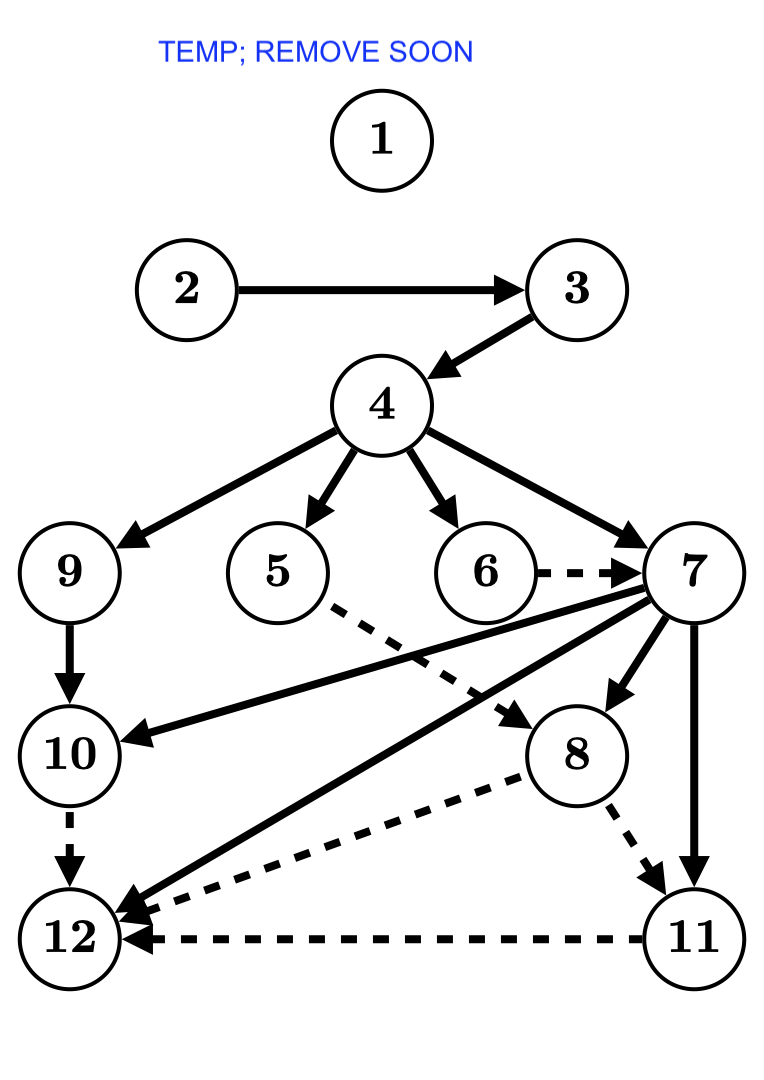
\includegraphics[width=\linewidth]{Interdependence.png}
    
    \newpage

    \textbf{Notes}:
    \interdependencenotes

    \mainmatter  % Now use arabic numerals for page numbers
}

%============= Index Pages ===============
\usepackage[
    totoc,
    columnsep=20pt,
    hangindent=8pt,
    subindent=20pt,
    subsubindent=30pt
]{idxlayout}

\makeindex[options= -s ../index-style.ist]

%======= Bibliography Formatting =========
% These two lines are here to ensure that URLs do not exceed the page by too much
\setcounter{biburllcpenalty}{7000}
\setcounter{biburlucpenalty}{8000}

\usepackage{xr}

\setasdraft  % TODO: Remove once no longer a draft

%=========== Global Variables ============
\newcommand{\version}{0.1}
\newcommand{\volumenumber}{2}
\newcommand{\volumename}{Rings}
\newcommand{\volumeimage}{cover/Integers Modulo n.png}

%============= Formatting ================
\linespread{1.05}

%============== Resources ================
\externaldocument{../Volume 0/number-theory}
\externaldocument{../Volume 0/polynomials}

\externaldocument{../Volume 1/basics-of-groups}
\externaldocument{../Volume 1/subgroups}
\externaldocument{../Volume 1/homomorphisms-and-isomorphisms}
\externaldocument{../Volume 1/more-groups}

%=========== Custom Commands =============
\newcommand{\ideal}[1]{\mathfrak{#1}}                % Ideal of a ring
\newcommand{\princ}[1]{\left\langle#1\right\rangle}  % Principal ideal generated by the element

\newcommand{\C}{\mathbb{C}}                        % The ring of complex numbers
\newcommand{\Mn}[2]{\mathcal{M}_{#1\times#1}(#2)}  % The ring of n by n matrices with entries in the ring R
\newcommand{\Q}{\mathbb{Q}}                        % The ring of rational numbers
\newcommand{\R}{\mathbb{R}}                        % The ring of real numbers
\newcommand{\Z}{\mathbb{Z}}                        % The ring of integers

\newcommand{\Ann}[2]{\mathrm{Ann}_{#1}(#2)}  % Annihilator of a subset A of a ring R
\newcommand{\Char}[1]{\mathrm{char}(#1)}     % Characteristic of a ring R
\newcommand{\Nilr}[1]{\mathfrak{N}_{#1}}     % Nilradical of a ring R

%========= Front Matter Pages ============
% Quote page
\newcommand{\quotepagetext}{
    [Some] of the major discoveries in ring theory have helped shape the course of development of modern abstract algebra... A course in ring theory is an indispensable part of the education of any fledgling algebraist.
}
\newcommand{\quotepageattribution}{Tsit-Yuen Lam, 2001}
\newcommand{\quotepagecitation}{\cite{lam_2001}}

% Preface
\newcommand{\prefacevolumetext}{
    This volume covers the basics of ring theory. %TODO: Add
}
\newcommand{\prefacevolumedate}{}  %TODO: Add

% Suggestions of use
\newcommand{\interdependencenotes}{
    % TODO: Update
}

%==== Include only relevant chapters =====
\IfFileExists{\jobname.run.xml}
{
    \includeonly{
        % Main chapters
        intro-to-rings,
        basics-of-rings,
        integral-domains,
        ideals-and-quotient-rings,
        ring-homomorphisms,
        polynomial-rings,
        % Appendices
        exercise-solutions,
        problem-solutions,
        appendices
    }
}
{
    % Do a full document initially to generate all the aux files
}

%=========================================
\begin{document}
\frontmatterpages

%=========================================
\chapter{Introduction to Rings}
In Volume I, we looked exclusively at groups and their operations. We discussed how groups are a generalisation of symmetry and looked at results related to groups. In this volume, we look at rings.

Before we introduce rings, we look at `simpler' algebraic structures and build our way up to them.

\section{Basic Algebraic Structures}
\begin{definition}
    A \textbf{magma}\index{magma} is a set $M$ together with a binary operation $\ast$ which is closed. That is, if $a$ and $b$ are in $M$, then $a \ast b \in M$. Such a magma is denoted $(M, \ast)$.
\end{definition}
\begin{example}
    Consider the set $M = \{1, 2, 3, 4\}$ with the operation $\ast$ such that $(M, \ast)$ has the Cayley table as shown below.
    \begin{table}[h]
        \centering
        \begin{tabular}{|l|l|l|l|l|}
            \hline
            $\ast$     & \textbf{1} & \textbf{2} & \textbf{3} & \textbf{4} \\ \hline
            \textbf{1} & 1          & 2          & 1          & 2          \\ \hline
            \textbf{2} & 2          & 3          & 4          & 1          \\ \hline
            \textbf{3} & 1          & 3          & 4          & 2          \\ \hline
            \textbf{4} & 2          & 1          & 2          & 1          \\ \hline
        \end{tabular}
    \end{table}
    
    Clearly for any $a, b\in M$ we have $a \ast b \in M$, so $(M, \ast)$ is a magma.
\end{example}

\begin{definition}
    A \textbf{semigroup}\index{semigroup} is a magma $(\mathcal{S}, \ast)$ where the operation $\ast$ is associative. That is, $a\ast(b\ast c) = (a\ast b)\ast c$.
\end{definition}
\begin{example}
    Consider the set $S = \{1, 2, 3, 4\}$ with the operation $\ast$ such that $(S, \ast)$ has the Cayley table as shown below.
    \begin{table}[h]
        \centering
        \begin{tabular}{|l|l|l|l|l|}
            \hline
            $\ast$     & \textbf{1} & \textbf{2} & \textbf{3} & \textbf{4} \\ \hline
            \textbf{1} & 1          & 1          & 1          & 1          \\ \hline
            \textbf{2} & 2          & 2          & 2          & 2          \\ \hline
            \textbf{3} & 3          & 3          & 3          & 3          \\ \hline
            \textbf{4} & 4          & 4          & 4          & 4          \\ \hline
        \end{tabular}
    \end{table}
    
    One sees that $(S, \ast)$ is closed under $\ast$. In addition, $\ast$ is associative. Hence $(S, \ast)$ is a semigroup.
\end{example}

\begin{definition}
    A \textbf{monoid}\index{monoid} is a semigroup $(M, \ast)$ with an element $e$, called the \textbf{identity}, such that
    \[
        e \ast m = m \ast e = m
    \]
    for all $m \in M$.
\end{definition}
\begin{example}
    The structure $(S, \circ)$, where
    \[
        S = \{f \vert  f: X \to X\},
    \]
    $X$ is a set, and $\circ$ denotes function composition forms a monoid.
    \begin{itemize}
        \item \textbf{Closure}: If $f, g \in S$ then $f\circ g \in S$ since function composition is closed.
        \item \textbf{Associative}: Function composition is associative.
        \item \textbf{Identity}: The identity function $\id: X \to X, x\mapsto x$ is inside $S$ and
        \[
            \id \circ f = f \circ \id = f
        \]
        for all $f \in S$.
    \end{itemize}
    Thus $(S, \circ)$ forms a monoid.
\end{example}

\begin{definition}
    A \textbf{group}\index{group} is a monoid $(G, \ast)$ where every element has an inverse. That is to say, for every $g \in G$, there exists $g^{-1} \in G$ such that
    \[
        g \ast g^{-1} = g^{-1} \ast g = e
    \]
    where $e$ is the identity in $G$.
\end{definition}

\section{Definition of a Ring}
With all that set up, we are ready to define what a ring is. Note that we follow \cite[p.~223]{dummit_foote_2004}, \cite[p.~115, Definition 1.1]{hungerford_1980}, and \cite{proofwiki_ring-definition} for the definition of a ring.
\begin{definition}
    A \textbf{ring}\index{ring} is a set $R$ with two binary operations $+$ and $\cdot$ satisfying the following axioms.
    \begin{itemize}
        \item \textbf{Addition-Abelian}: $(R, +)$ is an abelian group.
        \item \textbf{Multiplication-Semigroup}: $(R, \cdot)$ is a semigroup.
        \item \textbf{Distributive}: $\cdot$ is distributive over $+$. That is,
        \begin{itemize}
            \item $a \cdot (b + c) = (a \cdot b) + (b \cdot c)$; and
            \item $(a + b) \cdot c = (a \cdot c) + (b \cdot c)$.
        \end{itemize}
    \end{itemize}
    One may denote such a ring by $(R, +, \cdot)$.
\end{definition}
\begin{remark}
    Other authors (e.g. \cite[p.~136]{cohn_1982}, \cite[pp.~145--146]{clark_1984}) may require that $(R, \cdot)$ is a monoid. In this book, any ring that satisfies the above condition is called a \textbf{ring with identity}\index{ring!with identity}.
\end{remark}
\begin{remark}
    A ring where $a \cdot b = b \cdot a$ for all $a$ and $b$ in $R$ is called a \textbf{commutative ring}\index{ring!commutative}.
\end{remark}

We end this chapter by introducing the \textbf{trivial ring}.
\begin{definition}
    The \textbf{trivial ring}\index{trivial ring} (or \textbf{zero ring}\index{zero ring}), denoted $\textbf{0}$, is the ring $(\{0\}, +, \cdot)$ where
    \[
        0 + 0 = 0 \text{ and } 0 \cdot 0 = 0.    
    \]
\end{definition}
\begin{exercise}
    Prove that the trivial ring is a commutative ring with identity.
\end{exercise}

\chapter{Basics of Rings}
With an intuition and definition of rings out of the way, we are now ready to tackle the basics in this chapter.

\section{Obvious Rings}
Before we introduce some examples of rings, we make some remarks for the notation that is used in Ring Theory.
\begin{itemize}
    \item The multiplication symbol $\cdot$ is usually omitted, so $x \cdot y$ is written as $xy$.
    \item The additive identity of $R$ will always be denoted by 0 and the multiplicative identity of $R$ (if it exists) will always be denoted by 1.
    \item The additive inverse of the element $x$ will be denoted by $-x$ and the multiplicative inverse of $x$ (if it exists) will be denoted by $x^{-1}$.
    \item $n$ applications of $+$ on an element $x$ will be denoted $nx$ (and will be denoted $-nx$ if the element is $-x$), while $n$ applications of $\cdot$ on an element $x$ will be denoted $x^n$ (and will be denoted $x^{-n}$ if the element is $x^{-1}$ and if it exists).
\end{itemize}

Let's look at some examples of rings.
\begin{definition}
    The \textbf{ring of integers}\index{ring!of integers} is the set $\Z$ together with integer addition and multiplication.
\end{definition}
\begin{remark}
    We denote the ring of integers by $\Z$.
\end{remark}
\begin{proposition}
    $\Z$ is a commutative ring with identity.
\end{proposition}
\begin{proof}
    \myref{exercise-ring-of-integers-is-a-ring} (later) shows that $\Z$ is a ring. In addition, multiplication is commutative (\myref{axiom-multiplication-is-commutative}), and 1 is the multiplicative identity. Thus $\Z$ is a commutative ring with identity.
\end{proof}

\begin{definition}
    Let the integer $n > 2$. The \textbf{ring of integers modulo $n$}\index{ring!of integers!modulo $n$} is $(\Z_n, \oplus_n, \otimes_n)$, where $\oplus_n$ and $\otimes_n$ denote addition and multiplication modulo $n$ respectively.
\end{definition}
\begin{remark}
    We denote the ring of integers modulo $n$ by $\Z_n$.
\end{remark}
\begin{proposition}
    $\Z_n$ is a commutative ring with identity.
\end{proposition}
\begin{proof}
    We first prove the ring axioms before showing that it is commutative with a multiplicative identity.
    \begin{itemize}
        \item \textbf{Addition-Abelian}: We know $(\Z_n, \oplus_n)$ is an abelian group by \myref{prop-Zn-is-abelian-group}
        \item \textbf{Multiplication-Semigroup}: We can see that $(\Z_n, \otimes_n)$ is a semigroup as
        \begin{itemize}
            \item $\Z_n$ is closed under $\otimes_n$ because $a \otimes_n b \in \{0, 1, 2, \dots, n-1\} = \Z_n$; and
            \item multiplication is associative (\myref{axiom-multiplication-is-associative}), so multiplication modulo $n$ is associative.
        \end{itemize}
        \item \textbf{Distributive}: Since multiplication distributes over addition (\myref{axiom-distributivity}), thus multiplication modulo $n$ (i.e. $\otimes_n$) distributes over addition modulo $n$ (i.e. $\oplus_n$).
    \end{itemize}
    Hence $(\Z_n, \oplus_n, \otimes_n)$ is a ring.
    
    Furthermore, multiplication is commutative (\myref{axiom-multiplication-is-commutative}), so $\otimes_n$ is commutative. Also $\otimes_n$ has an identity of 1. Therefore $(\Z_n, \oplus_n, \otimes_n)$ is a commutative ring with identity.
\end{proof}

\begin{definition}
    The \textbf{ring of rational numbers}\index{ring!of rational numbers} is $(\Q, +, \times)$, where $+$ and $\times$ denote normal addition and multiplication.
\end{definition}
\begin{remark}
    We denote the ring of rational numbers by $(\Q, +, \times)$.
\end{remark}
\begin{proposition}
    $\Q$ is a commutative ring with identity.
\end{proposition}
\begin{proof}
    We first show that $\Q$ satisfies the ring axioms.
    \begin{itemize}
        \item \textbf{Addition-Abelian}: From part I, we know that $(\Q, +)$ is an abelian group.  % TODO: Add proof
        \item \textbf{Multiplication-Semigroup}: We note that $(\Q, \times)$ is a semigroup as
        \begin{itemize}
            \item $\Q$ is closed under $\times$ because multiplying two rational numbers together produce a rational number; and
            \item multiplication is associative (\myref{axiom-multiplication-is-associative}).
        \end{itemize}
        \item \textbf{Distributive}: Multiplication distributes over addition by \myref{axiom-distributivity}.
    \end{itemize}
    Hence $\Q$ is a ring. Furthermore, $\times$ has an identity of 1 and is commutative (\myref{axiom-multiplication-is-commutative}). So $\Q$ is a commutative ring with identity.
\end{proof}

\begin{definition}
    The \textbf{ring of real numbers}\index{ring!of real numbers} is the ring $(\R, +, \times)$ where $+$ and $\times$ denotes regular addition and multiplication respectively.
\end{definition}
\begin{remark}
    We denote the ring of real numbers by $(\R, +, \times)$.
\end{remark}
\begin{proposition}
    $\R$ is a commutative ring with identity.
\end{proposition}
\begin{proof}
    Replace $(\Q, +)$ with $(\R, +)$ and $(\Q, \times)$ with $(\R, \times)$ in the previous proof.
\end{proof}

We end this section by looking at the ring of complex numbers.
\begin{definition}
    Let the set of \textbf{complex numbers}\index{complex numbers}
    \[
        \C = \{a + bi \vert a, b \in \R\}
    \]
    where $i = \sqrt{-1}$ is known as the \textbf{imaginary unit}\index{imaginary unit}, where $i^2 = -1$. Define complex addition and multiplication by
    \begin{align*}
        (a+bi) + (c+di) &= (a+c) + (b+d)i,\\
        (a+bi) \cdot (c+di) &= (ac-bd) + (ad+bc)i.
    \end{align*}
    Then $\C$ under complex addition and multiplication is the \textbf{ring of complex numbers}\index{ring!of complex numbers}.
\end{definition}
\begin{remark}
    We denote the ring of complex numbers by $\C$.
\end{remark}
\begin{proposition}
    $\C$ is a commutative ring with identity.
\end{proposition}
\begin{proof}
    We first show that $\C$ satisfies the ring axioms.
    \begin{itemize}
        \item \textbf{Addition-Abelian}: We show that $(\C, +)$ satisfies the group axioms, and then show that $(\C, +)$ is commutative.
        \begin{itemize}
            \item \textbf{Closure}: Clearly for all real numbers $a$, $b$, $c$, and $d$ we have $a + c \in \R$ and $b+d \in \R$. Thus $(a+bi) + (c+di) = (a+c) + (b+d)i \in \C$, meaning $\C$ is closed under complex addition.
            
            \item \textbf{Associativity}: Let $a+bi, c+di, e+fi \in \C$. Then note that
            \begin{align*}
                &(a+bi) + ((c+di) + (e+fi))\\
                &= (a+bi) + ((c+e) + (d+f)i)\\
                &= (a+(c+e)) + (b+(d+f))i\\
                &= ((a+c)+e) + ((b+d)+f)i & (+ \text{ is associative, }\myref{axiom-addition-is-associative})\\
                &= ((a+c) + (b+d)i) + (e+fi)\\
                &= ((a+bi) + (c+di)) + (e+fi)
            \end{align*}
            so complex addition is associative.
            
            \item \textbf{Identity}: The identity in $\C$ is $0 + 0i = 0$ since
            \[
                (0+0i) + (a+bi) = (0+a) + (0+b)i = a+bi
            \]
            and complex addition is commutative (to be proved later), so $(\C,+)$ has an additive identity.
            
            \item \textbf{Inverse}: Let $a+bi \in \C$. Clearly $-a, -b \in \R$ and that
            \[
                (a+bi) + (-a+(-b)i)= (a+(-a)) + (b+(-b))i = 0
            \]
            and complex addition is commutative (to be proved later), so any $a+bi\in C$ has an additive inverse of $-a-bi \in \C$.

            \item \textbf{Commutative}: Let $a+bi, c+di \in \C$. Then
            \begin{align*}
                (a+bi) + (c+di) &= (a+c) + (b+d)i\\
                &= (c+a) + (d+b)i & (+\text{ is commutative, } \myref{axiom-addition-is-commutative})\\
                &= (c+di) + (a+bi)
            \end{align*}
            so complex addition is commutative.
        \end{itemize}
        
        \item \textbf{Multiplication-Semigroup}: We show that $(\C, \times)$ is a semigroup.
        \begin{itemize}
            \item \textbf{Closure}: Clearly for all real numbers $a$, $b$, $c$, and $d$ we have $ac, bd, ad, bc \in \R$, so $ac - bd, ad + bc \in \R$. Therefore
            \[
                (a+bi)(c+di) = (ac-bd) + (ad+bc)i \in \C
            \]
            which means $\C$ is closed under multiplication.

            \item \textbf{Associativity}: Let $a+bi, c+di, e+fi \in \C$. Note that
            \begin{align*}
                &(a+bi)((c+di)(e+fi))\\
                &= (a+bi)((ce-df)+(cf+de)i)\\
                &= (a(ce-df) - b(cf+de)) + (a(cf+de) + b(ce-df))i\\
                &= (ace - adf - bcf - bde) + (acf + ade + bce - bdf)i\\
                &= (ace - bde - adf - bcf) + (acf - bdf + ade + bce)i\\
                &= ((ac-bd)e - (ad+bc)f) + ((ac-bd)f + (ad+bc)e)i\\
                &= ((ac-bd)+(ad+bc)i)(e+fi)\\
                &= ((a+bi)(c+di))(e+fi)
            \end{align*}
            so complex multiplication is associative.
        \end{itemize}
        
        \item \textbf{Distributive}: We only prove left distributivity because we will show that complex multiplication is commutative later. Let $a+bi, c+di, e+fi \in \C$. Note that
        \begin{align*}
            &(a+bi)((c+di) + (e+fi))\\
            &= (a+bi)((c+e) + (d+f)i)\\
            &= (a(c+e)-b(d+f)) + (a(d+f) + b(c+e))i\\
            &= (ac+ae-bd-bf) + (ad+af+bc+be)i\\
            &= (ac-bd+ae-bf) + (ad+bc+af+be)i & (+ \text{ is associative})\\
            &= ((ac-bd) + (ad+bc)i) + ((ae - bf) + (af + be)i)\\
            &= (a+bi)(c+di) + (a+bi)(e+fi)
        \end{align*}
        so complex multiplication distributes over complex addition.
    \end{itemize}
    Hence $\C$ is a ring.
    
    \newpage
     
    We now show that complex multiplication is commutative. Let $a+bi, c+di \in C$. Then we see
    \begin{align*}
        (a+bi)(c+di) &= (ac-bd) + (ad+bc)i\\
        &= (ca-db) + (da+cb)i & (\times\text{ is commutative, } \myref{axiom-multiplication-is-commutative})\\
        &= (c+di)(a+bi)
    \end{align*}
    so complex multiplication is commutative.

    Finally we show that complex multiplication has an identity. Consider $1 + 0i \in \C$. Note that
    \[
        (1+0i)(a+bi) = (1a-0b) + (1b+0a)i = a+bi,
    \]
    and since complex multiplication is commutative, therefore $1+0i$ is the multiplicative identity in $\C$.
    
    Therefore $\C$ is a commutative ring with identity.
\end{proof}

These are just some examples of rings; we explore more later in this chapter.
\begin{exercise}\label{exercise-ring-of-integers-is-a-ring}
    Prove that $\Z$ is a ring under regular addition and multiplication.\newline
    (\textit{You do \textbf{not} need to prove the \textbf{Distributive} axiom.})
\end{exercise}

\section{General Properties of Rings}
We list some properties of rings here. For each of the propositions, assume $R$ is a ring.

\begin{proposition}\label{prop-multiplying-by-zero-is-zero}
    $0x = x0 = 0$ for all $x \in R$.
\end{proposition}
\begin{proof}
    We note that
    \begin{align*}
        0x &= (0 + 0)x & (0 \text{ is additive inverse})\\
        &= 0x + 0x & (\text{by \textbf{Distributive} axiom})
    \end{align*}
    so by `subtracting' $0x$ on both sides (i.e., adding $-0x$ on both sides) we see $0 = 0x$.
    
    Also
    \begin{align*}
        x0 &= x(0 + 0) & (0 \text{ is additive inverse})\\
        &= x0 + x0 & (\text{by \textbf{Distributive} axiom})
    \end{align*}
    so by `subtracting' $x0$ on both sides we see $0 = x0$.
    
    Therefore $0x = x0 = 0$ for all $x \in R$.
\end{proof}

\begin{proposition}\label{prop-product-of-element-and-additive-inverse-is-additive-inverse-of-product}
    $(-a)b = a(-b) = -(ab)$ for any $a$ and $b$ in $R$.
\end{proposition}
\begin{proof}
    We show that $(-a)b = -(ab)$ and $a(-b) = -(ab)$ to complete the proof.
    \begin{itemize}
        \item Note $(-a)b + ab = (-a + a)b = 0b = 0$ by \textbf{Distributive} axiom. Hence by subtracting $ab$ on both sides we see $(-a)b = -(ab)$.
        \item Note also $a(-b) + ab = a(-b + b) = a0 = 0$ by \textbf{Distributive} axiom. Hence by subtracting $ab$ on both sides we see $a(-b) = -(ab)$.
    \end{itemize}
    Result follows.
\end{proof}

\begin{proposition}
    $(-a)(-b) = ab$ for any $a$ and $b$ in $R$.
\end{proposition}
\begin{proof}
    See \myref{exercise-product-of-additive-inverses} (later).
\end{proof}

\begin{proposition}
    If $R$ has an identity, it is unique.
\end{proposition}
\begin{proof}
    Suppose 1 and $1'$ are identities, and consider the sum $1 + 1'$. Then
    \begin{align*}
        1 + 1' &= 1\times(1+1') & (\text{multiplying by identity }1)\\
        &= 1\times1 + 1\times1' & (\text{by \textbf{Distributive} axiom})\\
        &= 1 + 1. & (1 \text{ and } 1' \text{ are identities})
    \end{align*}
    Subtracting 1 on both sides yields $1 = 1'$, meaning that the identity is unique.
\end{proof}

\begin{exercise}\label{exercise-product-of-additive-inverses}
    Show that $(-a)(-b) = ab$ for any $a$ and $b$ in $R$.
\end{exercise}

% \section{Some Non-Obvious Rings}
\section{Matrix Rings}
The rings that we explored in previous sections can be thought of as the `obvious' rings, since they are number systems. As rings were made to generalize number systems, they should clearly be rings. However, there are less obvious rings.

% \subsection{Matrix Rings}
We looked at matrices in the context of the General/Special Linear Group of matrices. Here we see that matrices in fact form rings, known as matrix rings. Before that though, we need to define the operations within that ring.

\begin{definition}[Matrix Addition]\index{matrix addition}
    For any two matrices $\textbf{A}$ and $\textbf{B}$ with $n$ rows and columns and entries in the ring $(R, \oplus, \otimes)$, their sum is the matrix $\textbf{C} = \textbf{A} + \textbf{B}$ with $n$ rows and columns such that
    \[
        c_{i,j} = a_{i,j} \oplus b_{i,j}
    \]
    for all $i,j \in \{1, 2, \dots, n\}$.
\end{definition}
\begin{definition}[Matrix Multiplication]\index{matrix multiplication}
    For any two matrices $\textbf{A}$ and $\textbf{B}$ with $n$ rows and columns and entries in the ring $(R, \oplus, \otimes)$, their product is the matrix $\textbf{C} = \textbf{AB}$ with $n$ rows and columns such that, for all $i,j \in \{1, 2, \dots, n\}$, we have
    \begin{align*}
        c_{i,j} &= (a_{i,1}\otimes b_{1,j}) \oplus (a_{i,2}\otimes b_{2,j}) \oplus \cdots \oplus (a_{i,n}\otimes b_{n,j})\\
        &= \bigoplus_{k=1}^n (a_{i,k}\otimes b_{k,j}).
    \end{align*}
\end{definition}

We also define two matrices that will become useful when we work with matrix rings.
\begin{definition}
    The \textbf{zero matrix}\index{zero matrix} with $n$ rows and columns is
    \[
        \ZeroM{n} = 
        \begin{pmatrix}
            0 & 0 & 0 & \cdots & 0 \\
            0 & 0 & 0 & \cdots & 0 \\
            0 & 0 & 0 & \cdots & 0 \\
            \vdots & \vdots & \vdots & \ddots & \vdots \\
            0 & 0 & 0 & \cdots & 0 \\
        \end{pmatrix}
    \]
    where 0 is the additive identity (i.e. zero) in the ring $(R, \oplus, \otimes)$.
\end{definition}
\begin{definition}
    The \textbf{identity matrix}\index{identity matrix} with $n$ rows and columns is
    \[
        \IdentityM{n} = 
        \begin{pmatrix}
            1 & 0 & 0 & \cdots & 0 \\
            0 & 1 & 0 & \cdots & 0 \\
            0 & 0 & 1 & \cdots & 0 \\
            \vdots & \vdots & \vdots & \ddots & \vdots \\
            0 & 0 & 0 & \cdots & 1 \\
        \end{pmatrix}
    \]
    where 0 and 1 are the additive and multiplicative identities (i.e. zero and one) in the ring $(R, \oplus, \otimes)$ respectively. That is, the identity matrix is the matrix with 1s in the leading diagonal.
\end{definition}

We can now define what is a matrix ring.
\begin{definition}
    Let $(R, \oplus, \otimes)$ be a ring and $n$ be a positive integer. Then $\Mn{n}{R}$ under matrix addition and multiplication is a ring, known as the \textbf{matrix ring}\index{matrix ring} with elements in $(R, \oplus, \otimes)$.
\end{definition}
\begin{proposition}
    $\Mn{n}{R}$ is a ring with identity.
\end{proposition}
\begin{proof}
    We need to prove that the ring axioms hold.
    \begin{itemize}
        \item \textbf{Addition-Abelian}: We first prove that $(\Mn{n}{R}, +)$ is indeed an abelian group.
        \begin{itemize}
            \item \textbf{Closure}: Clearly the sum of any two matrices in $\Mn{n}{R}$ is also a square matrix with $n$ rows with elements inside $R$, meaning that $\Mn{n}{R}$ is closed under matrix addition.

            \item \textbf{Associative}: Let the matrices $\textbf{A}$, $\textbf{B}$, and $\textbf{C}$ belong inside $\Mn{n}{R}$. Let $\textbf{P} = \textbf{A} + (\textbf{B} + \textbf{C})$ and $\textbf{Q} = (\textbf{A} + \textbf{B}) + \textbf{C}$. We note that $\textbf{P} = \textbf{Q}$ as
            \[
                p_{i,j} = a_{i,j} \oplus (b_{i,j} \oplus c_{i,j}) = (a_{i,j} \oplus b_{i,j}) \oplus c_{i,j} = q_{i,j}
            \]
            by associativity of $\oplus$, which proves that matrix addition is associative.
    
            \item \textbf{Identity}: We show that $\ZeroM{n}$ is the additive identity in $\Mn{n}{R}$. Let $\textbf{M} \in \Mn{n}{R}$; let $\textbf{N} = \textbf{M} + \ZeroM{n}$. Note that $n_{i,j} = m_{i,j} \oplus 0 = m_{i,j}$ so $\textbf{M} + \ZeroM{n} = \textbf{M}$. Therefore $\textbf{M} + \ZeroM{n} = \textbf{M}$ for any matrix in $\Mn{n}{R}$.
            
            \item \textbf{Inverse}: Let $\textbf{A} \in \Mn{n}{R}$. Define the matrix $\textbf{B} = -\textbf{A}$ such that $b_{i,j} = -a_{i,j}$. That is, $b_{i,j}$ contains the additive inverse of $a_{i,j}$ in the ring $R$. Then one sees that $\textbf{A} + \textbf{B} = \ZeroM{n}$. (We denote the additive inverse of a matrix $\textbf{M}$ by $-\textbf{M}$).

            \item \textbf{Commutative}: Let $\textbf{A}, \textbf{B} \in \Mn{n}{R}$. Set $\textbf{C} = \textbf{A} + \textbf{B}$ and $\textbf{D} = \textbf{B} + \textbf{C}$. Consider $c_{i,j} = a_{i,j} \oplus b_{i,j}$. Since $\oplus$ is commutative, thus $a_{i,j} \oplus b_{i,j} = b_{i,j} \oplus a_{i,j}$. But $d_{i,j} = b_{i,j} \oplus a_{i,j}$, so we have $c_{i,j} = d_{i,j}$. Therefore $\textbf{C} = \textbf{D}$.
        \end{itemize}

        \item \textbf{Multiplication-Semigroup}: We show that $(\Mn{n}{R}, \cdot)$ is a semigroup.
        \begin{itemize}
            \item \textbf{Closure}: In \myref{subsection-intro-to-matrices} we showed that matrix multiplication produces another $n \times n$ matrix. Furthermore the entries of the new matrix are elements of $R$. Hence $\Mn{n}{R}$ is closed under matrix multiplication.
        
            \item \textbf{Associative}: We proved matrix multiplication is associative in \myref{subsection-GLR-matrix-group}.
        \end{itemize}
        
        \item \textbf{Distributive}: We prove only $\textbf{A}(\textbf{B} + \textbf{C}) = (\textbf{AB}) + (\textbf{AC})$ as the other case is proven similarly. Let $\textbf{R} = \textbf{A}(\textbf{B} + \textbf{C})$, $\textbf{G} = \textbf{AB}$, and $\textbf{H} = \textbf{AC}$. We note
        \begin{align*}
            r_{i,j} &= \bigoplus_{k=1}^n \left(a_{i,k} \otimes \left(b_{k,j} \oplus c_{k,j}\right)\right)\\
            &= \bigoplus_{k=1}^n \left((a_{i,k} \otimes b_{k,j}) \oplus (a_{i,k} \otimes c_{k,j})\right)\\
            &= \left(\bigoplus_{k=1}^n (a_{i,k} \otimes b_{k,j})\right) \oplus \left(\bigoplus_{k=1}^n (a_{i,k} \otimes c_{k,j})\right)\\
            &= g_{i,j}\oplus h_{i,j}
        \end{align*}
        which means $\textbf{R} = \textbf{G} + \textbf{H}$.
    \end{itemize}
    As all the ring axioms are satisfied, thus $\Mn{n}{R}$ is a ring.

    We now show that $\Mn{n}{R}$ has a multiplicative identity, namely the identity matrix $\IdentityM{n}$. Let $\textbf{A} \in \Mn{n}{R}$ and let $\textbf{B} = \IdentityM{n}$. Note that $b_{i,j} = 1$ if and only if $i = j$.
    \begin{itemize}
        \item Let $\textbf{C} = \textbf{AB}$ and we see
        \begin{align*}
            &c_{i,j}\\
            &= \bigoplus_{k=1}^n(a_{i,k}\otimes b_{k,j})\\
            &= (a_{i,1}\otimes b_{1,j}) \oplus \cdots \oplus (a_{i,j-1}\otimes b_{j-1,j}) \oplus (a_{i,j}\otimes b_{j,j})\\
            &\quad\quad\oplus (a_{i,{j+1}}\otimes b_{j+1,j}) \oplus \cdots \oplus (a_{i,n}\otimes b_{n,j})\\
            &= (a_{i,1}\otimes 0) \oplus \cdots \oplus (a_{i,{j-1}}\otimes 0)\oplus (a_{i,j}\otimes 1) \oplus (a_{i,{j+1}}\otimes 0) \oplus \cdots \oplus (a_{i,n}\otimes 0)\\
            &= 0 \oplus \cdots \oplus 0 \oplus a_{i,j} \oplus 0 \oplus \cdots \oplus 0\\
            &= a_{i,j}
        \end{align*}
        so $\textbf{A}\IdentityM{n} = \textbf{A}$.

        \item Now let $\textbf{D} = \textbf{BA}$ and we also see
        \begin{align*}
            &d_{i,j}\\
            &= \bigoplus_{k=1}^n(b_{i,k}\otimes a_{k,j})\\
            &= (b_{i,1}\otimes a_{1,j}) \oplus \cdots \oplus (b_{i,i-1}\otimes b_{i-1,j}) \oplus (b_{i,i}\otimes a_{i,j})\\
            &\quad\quad\oplus (b_{i,{i+1}}\otimes a_{i+1,j}) \oplus \cdots \oplus (b_{i,n}\otimes a_{n,j})\\
            &= (0 \otimes a_{1,j}) \oplus \cdots \oplus (0\otimes a_{i-1,j})\oplus (1\otimes a_{i,j}) \oplus (0\otimes a_{i+1,j}) \oplus \cdots \oplus (0\otimes a_{n,j})\\
            &= 0 \oplus \cdots \oplus 0 \oplus a_{i,j} \oplus 0 \oplus \cdots \oplus 0\\
            &= a_{i,j}
        \end{align*}
        so $\IdentityM{n}\textbf{A} = \textbf{A}$.
    \end{itemize}
    Therefore the identity matrix $\IdentityM{n}$ is the multiplicative identity.

    Hence $\Mn{n}{R}$ is a ring with identity.
\end{proof}

% \subsection{Hamilton's Quaternions}
% The quaternions is a way to extend the complex numbers into 4 dimensions. Irish mathematician William Rowan Hamilton was looking for a way represent points in 3-dimensional space using numbers. He knew how to add and subtract triples of numbers, but had difficulty in defining a way to multiply and divide these numbers, just like in the ring of complex numbers. The breakthrough in quaternions came in 1843 when he thought of using 4-dimensional numbers instead of 3-dimensional numbers.

% We define what quaternions are, and what the quaternion ring is.
% \begin{definition}
%     A \textbf{quaternion}\index{quaternion} is an expression of the form
%     \[
%         a + b\qi + c\qj + d\qk
%     \]
%     where $a,b,c,d \in \R$ and $\qi$, $\qj$, and $\qk$ are quantities such that
%     \begin{itemize}
%         \item $\qi\qj = -\qj\qi = \qk$;
%         \item $\qj\qk = -\qk\qj = \qi$;
%         \item $\qk\qi = -\qi\qk = \qj$; and
%         \item $\qi^2 = \qk^2 = \qk^2 = \qi\qj\qk = -1$.
%     \end{itemize}
% \end{definition}
% \begin{definition}
%     The \textbf{quaternion ring}\index{quaternion ring} is
%     \[
%         \H = \{a + b\qi + c\qj + d\qk \vert a,b,c,d \in \R\}
%     \]
%     where, for two quaternions $q_1 = a_1+b_1\qi+c_1\qj+d_1\qk$ and $q_2 = a_2+b_2\qi+c_2\qj+d_2\qk$, addition is
%     \[
%         q_1 + q_2 = (a_1+a_2) + (b_1+b_2)\qi + (c_1+c_2)\qj + (d_1+d_2)\qk
%     \]
%     and multiplication is
%     \begin{align*}
%         q_1q_2 &= (a_1a_2 - b_1b_2 - c_1c_2 - d_1d_2)\\
%         &+(a_1b_2 + b_1a_2 + c_1d_2 - d_1c_2)\qi\\
%         &+(a_1c_2 - b_1d_2 + c_1a_2 + d_1b_2)\qj\\
%         &+(a_1d_2 + b_1c_2 - c_1b_2 + d_1a_2)\qk.
%     \end{align*}
% \end{definition}

\section{More Definitions}
Suppose $R$ is a ring.
\begin{definition}
    We say that $a \neq 0$ is a \textbf{zero divisor}\index{zero divisor} in $R$ if there exists $b \neq 0$ such that $ab = 0$.
\end{definition}
\begin{example}
    Consider the ring $\Z_{12}$. Clearly 4 and 6 are in $\Z_{12}$, and their product is $24 = 2 \times 12 = 0$ in $\Z_{12}$. Hence 4 and 6 are zero divisors in $\Z_{12}$.
\end{example}
\begin{example}
    Let $R$ be the ring of functions with domain and codomain $[0, 1]$. We claim that $R$ has zero divisors. Consider the functions
    \begin{align*}
        f:[0,1]\to[0,1], x &\mapsto x\\
        g:[0,1]\to[0,1], x &\mapsto \begin{cases}
            0 & \text{ if } x \neq 0\\
            1 & \text{ if } x = 0
        \end{cases}
    \end{align*}
    Clearly neither of them are the zero function. However, consider $f(x)g(x)$.
    \begin{itemize}
        \item If $x \neq 0$, then $g(x) = 0$ which means $f(x)g(x) = 0$.
        \item If $x = 0$, then $f(x) = 0$ which means $f(x)g(x) = 0$.
    \end{itemize}
    Hence their product is the zero function, meaning that $R$ has zero divisors $f$ and $g$.
\end{example}
\begin{exercise}
    Does the ring $\Mn{2}{\mathbb{R}}$ have zero divisors?
\end{exercise}
We note one property about zero divisors, which will be used in future chapters.
\begin{proposition}\label{prop-zero-divisors-have-no-inverses}
    Zero divisors do not have inverses.
\end{proposition}
\begin{proof}
    Assume $a \neq 0$ and $b \neq 0$ are zero divisors in the ring $R$, so $ab = 0$. Seeking a contradiction, assume $a$ has an inverse, so
    \[
        b = (a^{-1}a)b = a^{-1}(ab) = a^{-1}0 = 0    
    \]
    which contradicts $b \neq 0$. Hence a zero divisor has no inverse.
\end{proof}

\begin{definition}
    Suppose $R$ is a ring with identity such that $0 \neq 1$. An element $u \in R$ is called a \textbf{unit}\index{unit} if there exists a $v \in R$ such that $uv=vu=1$. Equivalently, $u$ is a unit if it has a multiplicative inverse.
\end{definition}
\begin{example}
    3 and 7 are units in $\Z_{10}$ since $3 \times 7 = 7 \times 3 = 21 = 1$ in $\Z_{10}$.
\end{example}

\begin{definition}
    Suppose $R$ is a ring with identity such that $0 \neq 1$. If every non-zero element $x \in R$ is a unit, then $R$ is said to be a \textbf{division ring}\index{division ring}.
\end{definition}

\begin{definition}
    A commutative division ring is called a \textbf{field}\index{field}.
\end{definition}
We look at fields in more detail in part III.

\begin{exercise}\label{exercise-Z-is-not-a-field}
    Is $\Z$ a field?
\end{exercise}

\section{Subrings}
We end this chapter off with an exploration about subrings.

\begin{definition}
    Let $R$ be a ring and $S$ be a subset of $R$. Then $S$ is a \textbf{subring}\index{subring} of $R$ if
    \begin{itemize}
        \item $(S, +) \leq (R, +)$, that is, the subset $S$ under addition is a subgroup of $R$ under addition; and
        \item for all $a$ and $b$ in $S$ we have $ab \in S$, i.e. $S$ is closed under multiplication.
    \end{itemize}
\end{definition}
\begin{remark}
    Alternatively, one may show that $S$ is a ring to prove that $S$ is a subring of $R$.
\end{remark}

\begin{example}
    We know that $\Z$ and $\Q$ are rings, and clearly $\Z \subseteq \Q$. Hence $\Z$ is a subring of $\Q$. Similarly, since $\Q \subseteq \R$ and $\R \subseteq \C$, thus $\Q$ is a subring of $\R$ and $\R$ is a subring of $\C$.
\end{example}

\begin{example}
    Consider the set of \textbf{gaussian integers}\index{gaussian integers}
    \[
        \Z[i] = \{a + bi \vert a,b\in\mathbb{Z}\},
    \]
    read as ``$\Z$ adjoin $i$''. We first show that $\Z[i]$ is a subring of $\C$.
    \begin{proof}
        Clearly $\Z[i] \subseteq \C$. We show that $(\Z[i], +) \leq (\C, +)$.
        \begin{itemize}
            \item Clearly the identity of $(\C, +)$, which is 0, is inside $(\Z[i], +)$ as $0 = 0 + 0i$.
            \item For any $a + bi, c+di \in \Z[i]$, we have
            \[
                (a+bi) + (-(c+di)) = (a-c) + (b-d)i \in \Z[i].
            \]
        \end{itemize}
        Thus the subgroup test (\myref{thrm-subgroup-test}) tells us that $(\Z[i], +) \leq (\C, +)$.

        Now we show that $\Z[i]$ is closed under multiplication. Let $a + bi, c+di \in \Z[i]$. Note that $ac, bd, ad, bc \in \Z$; the product of the two gaussian integers is
        \begin{align*}
            (a+bi)(c+di) &= (ac-bd) + (ad+bc)i\\
            &\in \Z[i]
        \end{align*}
        so $\Z[i]$ is closed under multiplication.
        
        Therefore $\Z[i]$ is a subring of $\C$.
    \end{proof}
\end{example}
\begin{exercise}
    Show that
    \[
        R = \left\{\begin{pmatrix}a&a\\a&a\end{pmatrix} \vert a \in \R\right\}
    \]
    is a subring of $\Mn{2}{\mathbb{R}}$.
\end{exercise}

\newpage

\section{Problems}
\begin{problem}
    Let $R$ be a ring. Prove that if $u \in R$ is a unit then so is $-u$.
\end{problem}

\begin{problem}
    Prove that the trivial ring is the unique ring with identity in which $0 = 1$.
\end{problem}

\begin{problem}
    Let $R$ be a set with an operation $\ast$ such that for all elements $x$ and $y$ in $R$ we have $x \ast y \in R$. If $(R, \ast, \ast)$ is a ring, describe the elements in $R$.
\end{problem}

\begin{problem}
    Prove that it is impossible for an element of a ring $R$ to be both a zero divisor and a unit.
\end{problem}

\begin{problem}
    Let $R$ be a ring with identity 1, and let $x$ be an element from that ring.
    \begin{partquestions}{\roman*}
        \item Find \textbf{four} closed forms for the geometric series $1 + x + x^2 + x^3 + \cdots + x^n$.
        \item What are the condition(s) such that the closed forms are valid?
        \item Evaluate 112 in the ring $\Z_{37}$.
        \item Hence, using the result(s) above, evaluate
        \[
            1 + 2^3 + 2^6 + 2^9 + \cdots + 2^{72}
        \]
        in the ring $\Z_{37}$.
    \end{partquestions}
\end{problem}

\begin{problem}
    Show that
    \[
        \Q[\sqrt2] = \{a + b\sqrt2 \vert a,b \in \Q\}
    \]
    is a ring. Hence show it is a field.
\end{problem}

\begin{problem}
    Let
    \[
        R = \left\{\begin{pmatrix}a&b\\0&0\end{pmatrix} \vert a,b \in \R\right\}    
    \]
    be a ring under matrix addition and multiplication.
    \begin{partquestions}{\roman*}
        \item Show that $R$ has no identity.
        \item Show that $R$ contains a non-trivial subring $S$ with identity.
    \end{partquestions}
\end{problem}

\begin{problem}
    A ring $R$ is called a \textbf{Boolean ring}\index{Boolean ring} if $r^2 = r$ for all $r \in R$.
    \begin{partquestions}{\roman*}
        \item Show that $r = -r$ for all $r \in R$.
        \item Prove that every Boolean ring is commutative.
    \end{partquestions}
\end{problem}

\begin{problem}
    Let $R$ be a commutative ring with identity. We say that an element $x$ in $R$ is \textbf{nilpotent}\index{nilpotent} if there exists a positive integer $n$ such that $x^n = 0$.
    \begin{partquestions}{\roman*}
        \item Show that the product of two units is a unit.
        \item Let $u \in R$ be a unit and $x \in R$ be nilpotent. Show that $ux$ is nilpotent.
        \item Show that $u - x$ is a unit.
    \end{partquestions}
\end{problem}

\chapter{Integral Domains}
Unlike groups, rings do not inherently have the `cancellation law' built in. Rings may have zero divisors, which break the cancellation law. We look at a special category of rings, called domains, and commutative domains, called integral domains.

\section{What are Domains and Integral Domains?}
\begin{definition}
    A \term{domain}\index{domain!ring} is a ring with identity without zero divisors.
\end{definition}
\begin{remark}
    Recall that a non-zero element $a$ is a zero divisor if there exists a non-zero $b$ in the ring such that $ab = 0$. So, equivalently, if $a \neq 0$ and $b \neq 0$ then $ab \neq 0$ for any $a$ and $b$ in the domain.
\end{remark}
\begin{remark}
    What this property grants us is a ``cancellation law'', similar to that for groups. We will prove this in \myref{prop-domain-cancellation-law}. However, there may not be inverses when performing multiplication.
\end{remark}

\begin{definition}
    An \term{integral domain}\index{integral domain} is a commutative domain.
\end{definition}
\begin{remark}
    This is similar to how the only way for two integers to multiply to zero is if both integers are zero, hence the name ``integral domain''.
\end{remark}

\begin{example}\label{example-integers-is-integral-domain}
    We show that the integers, $\Z$, the namesake for integral domains, is indeed an integral domain. We note that $\Z$ is a commutative ring as multiplication is commutative. Furthermore, 1 is the multiplicative identity in $\Z$. All that remains is to show that there does not exist any zero divisors in $\Z$.

    Suppose $a$ and $b$ are non-zero elements in $\Z$. We show that $ab \neq 0$ to prove that there does not exist any zero divisors. Let's first consider the case when $b > 0$. We may write
    \[
        ab = \underbrace{a + a + \cdots + a}_{b \text{ times}}
    \]
    which clearly is not zero since $a \neq 0$. Now if $b < 0$ then note
    \[
        ab = (-a)(-b) = \underbrace{(-a) + (-a) + \cdots + (-a)}_{(-b) \text{times}}
    \]
    which is also not zero as $-a \neq 0$. Hence there are no zero divisors in $\Z$.

    Therefore $\Z$ is a commutative ring with identity without any zero divisors, meaning that $\Z$ is an integral domain.
\end{example}

\begin{example}
    We show that the ring $\Z[i]$, the Gaussian integers, is an integral domain. Similar to $\Z$, we note multiplication is commutative with identity 1.

    Suppose $w$ and $z$ are non-zero elements in $\Z[i]$; write $w = a+bi$ and $z = c+di$. Note that $a^2+b^2 \neq 0$ and $c^2 + d^2 \neq 0$. By definition of complex multiplication we have
    \[
        wz = (a+bi)(c+di) = (ac-bd) + (ad+bc)i.
    \]
    We just need to show that $ac-bd \neq 0$ and $ad+bc \neq 0$. Note that for any real numbers $x$ and $y$, we have $x^2 + y^2 \neq 0$ if and only if both $x$ and $y$ are non-zero. So we see
    \begin{align*}
        (ac-bd)^2 + (ad+bc)^2 &= (a^2c^2 - 2abcd + b^2d^2) + (a^2d^2 + 2abcd + b^2c^2)\\
        &= a^2c^2 + a^2d^2 + b^2c^2 + b^2d^2\\
        &= (a^2 + b^2)(c^2 + d^2)\\
        &\neq 0
    \end{align*}
    which hence means that $ac-bd \neq 0$ and $ad+bc \neq 0$. Therefore $wz \neq 0$, meaning that $\Z[i]$ has no zero divisors. Thus $\Z[i]$ is indeed an integral domain.
\end{example}

Let's look at some non-examples of domains.
\begin{example}
    The ring $\Mn{n}{R}$ where $R$ is any ring and $n$ is any integer greater than 1 is not a domain since, for $n = 2$, we have the non-zero matrices
    \[
        A = \begin{pmatrix}0&0\\0&1\end{pmatrix} \text{ and } B = \begin{pmatrix}1&0\\0&0\end{pmatrix}
    \]
    which have a product that is the zero matrix. Thus $\Mn{n}{R}$ has zero divisors, meaning that $\Mn{n}{R}$ is not a domain (and hence not an integral domain).
\end{example}
\begin{example}
    The ring $2\Z$ is not a domain as it does not contain a multiplicative identity (namely, 1). Thus $2\Z$ is also not an integral domain.
\end{example}
\begin{example}
    The ring $\Z \times \Z$ under pairwise addition and multiplication is not a domain as $(0,1) \neq (0, 0)$ and $(1, 0) \neq (0, 0)$ but $(0,1)(1,0) = (0, 0)$, meaning that $\Z \times \Z$ contains a zero divisor.
\end{example}

\begin{exercise}
    Prove that the ring
    \[
        \Z[\sqrt2] = \left\{a + b\sqrt2 \vert a,b \in \Z\right\}
    \]
    is an integral domain.
\end{exercise}
\begin{exercise}
    Let $n$ be a composite number. Prove that $\Z_n$ is not an integral domain.
\end{exercise}

We note an interesting result regarding fields here.
\begin{proposition}\label{prop-field-is-integral-domain}
    Any field is an integral domain.
\end{proposition}
\begin{proof}
    Any non-zero element in a field is a unit, i.e. has an inverse. Now by \myref{prop-zero-divisors-have-no-inverses}, any zero divisor must not have an inverse; the contrapositive being that any element that has an inverse cannot be a zero divisor. Hence, there are no zero divisors in a field. Now a field is commutative, therefore meaning that the field is an integral domain.
\end{proof}

\section{General Properties and Results}
With an introduction of domains and integral domains out of the way, we introduce some general results applicable to them.
\begin{proposition}[Cancellation Law for Domains]\index{cancellation law!domains}\label{prop-domain-cancellation-law}
    Let $D$ be a domain, $r, x, y \in D$, and $r \neq 0$. Then the following statements are equivalent.
    \begin{enumerate}
        \item $x = y$
        \item $rx = ry$
        \item $xr = yr$
    \end{enumerate}
\end{proposition}
\begin{proof}
    We prove the statements in order.
    \begin{itemize}
        \item $\boxed{(1) \implies (2)}$ Given $x = y$, this means $x - y = 0$. Multiplying $r$ on the left on both sides yields $r(x-y) = r0 = 0$. Distributing yields $rx - ry = 0$ which hence means $rx = ry$.

        \item $\boxed{(2) \implies (3)}$ Given $rx = ry$. Multiplying $r$ on the right on both sides yields $rxr = ryr$, thereby meaning $rxr - ryr = 0$. Factoring yields $r(xr - yr) = 0$. As $R$ is a domain, the only way for this to occur is if $r = 0$ (which is impossible) or $xr - yr = 0$. Therefore $xr = yr$.

        \item $\boxed{(3) \implies (1)}$ Given $xr = yr$ we may write $xr - yr = (x-y)r = 0$. Since $R$ is a domain we must have $x - y = 0$ or $r = 0$ (impossible as $r \neq 0$). Hence $x = y$.
    \end{itemize}
    This proves the proposition.
\end{proof}

\begin{theorem}\label{thrm-finite-integral-domain-is-field}
    Every finite integral domain is a field.
\end{theorem}
\begin{proof}
    A finite integral domain is a commutative ring with identity; all that remains is to prove that every non-zero element has an inverse.

    Suppose $D$ is a finite integral domain and take a non-zero element $r \in D$. Consider
    \begin{align*}
        A &= \{r^k \vert k \in \Z,\;k\geq 0\}\\
        &= \{1, r, r^2, r^3, \dots\}\\
        &\subseteq D.
    \end{align*}
    Note that since $D$ is finite, $A$ must be finite as well. Therefore there must exist positive integers $m$ and $n$ with $m > n$ such that $r^m = r^n$, meaning $r^m - r^n = 0$. As $m > n$, thus $r^n\left(r^{m-n}-1\right) = 0$. Hence, as there are no zero divisors in $R$, either $r^n = 0$ or $r^{m-n} - 1 = 0$.

    Now, seeking a contradiction, suppose $r^n = 0$. Then $n > 1$ since $r^1 = r \neq 0$ by assumption. Note $r^n = rr^{n-1} = 0$, which hence means $r^{n-1} = 0$ as $r \neq 0$ and $D$ has no zero divisors. But we may repeat this argument on $n - 1$ to eventually terminate at $r = 0$, which is a contradiction. Hence we must conclude that $r^{m-n} - 1 = 0$. We may write $r^{m-n}-1 = 0$ as $rr^{m-n-1} = 1$ which means that $r$ is a unit (with $r^{m-n-1}$ is its inverse). Therefore every non-zero element has an inverse.

    Hence $D$ is a field.
\end{proof}

\begin{remark}
    We note that finite fields are also known as \term{Galois fields}\index{Galois Field}, so-named in honour of \'Evariste Galois. We explore more properties of fields and Galois fields in part III.
\end{remark}

\begin{example}\label{example-Zp-is-field}
    Let $p$ be a prime and consider the ring $\Z_p$. Clearly multiplication is commutative with identity 1. We just need to show that $\Z_p$ has no zero divisors. So suppose $a,b \in \Z_p$ such that $ab = 0$ in $\Z_p$. Thus $ab = pk$ for some integer $k$; Euclid's lemma (\myref{corollary-euclid}) tells us that $p \vert a$ or $p \vert b$, which means $a = 0$ or $b = 0$ in $\Z_p$. Thus there are no zero divisors in $\Z_p$, so $\Z_p$ is an integral domain. Now $\Z_p$ is finite as it only has $p$ elements; by \myref{thrm-finite-integral-domain-is-field} we know that $\Z_p$ is a field.
\end{example}

\begin{example}
    We show that $\Z_3[i] = \{a+bi \vert a,b \in \Z_3\}$ is a finite integral domain in order to show that it is a field. Clearly multiplication is commutative with identity 1, so we just need to show that there are no zero divisors in $\Z_3[i]$.
    \begin{table}[h]
        \centering
        \resizebox{\textwidth}{!}{
            \begin{tabular}{|l|l|l|l|l|l|l|l|l|}
            \hline
            $\boldsymbol{\times}$ & $\boldsymbol{1}$ & $\boldsymbol{2}$ & $\boldsymbol{i}$ & $\boldsymbol{1+i}$ & $\boldsymbol{2+i}$ & $\boldsymbol{2i}$ & $\boldsymbol{1+2i}$ & $\boldsymbol{2+2i}$ \\ \hline
            $\boldsymbol{1}$    & 1      & 2      & $i$    & $1+i$  & $2+i$  & $2i$   & $1+2i$ & $2+2i$ \\ \hline
            $\boldsymbol{2}$    & 2      & 1      & $2i$   & $2+2i$ & $1+2i$ & $i$    & $2+i$  & $1+i$  \\ \hline
            $\boldsymbol{i}$    & $i$    & $2i$   & 2      & $2+i$  & $2+2i$ & 1      & $1+i$  & $1+2i$ \\ \hline
            $\boldsymbol{1+i}$  & $1+i$  & $2+2i$ & $2+i$  & $2i$   & 1      & $1+2i$ & 2      & $i$    \\ \hline
            $\boldsymbol{2+i}$  & $2+i$  & $1+2i$ & $2+2i$ & 1      & $i$    & $1+i$  & $2i$   & 2      \\ \hline
            $\boldsymbol{2i}$   & $2i$   & $i$    & 1      & $1+2i$ & $1+i$  & 2      & $2+2i$ & $2+i$  \\ \hline
            $\boldsymbol{1+2i}$ & $1+2i$ & $2+i$  & $1+i$  & 2      & $2i$   & $2+2i$ & $i$    & 1      \\ \hline
            $\boldsymbol{2+2i}$ & $2+2i$ & $1+i$  & $1+2i$ & $i$    & 2      & $2+i$  & 1      & $2i$   \\ \hline
            \end{tabular}
        }
    \end{table}

    From the table, we have shown that no two non-zero elements in $\Z_3[i]$ multiply to zero. Therefore $\Z_3[i]$ has no zero divisors, which means $\Z_3[i]$ is an integral domain. Furthermore, as $\Z_3[i]$ is finite, therefore it is a finite field by \myref{thrm-finite-integral-domain-is-field}.
\end{example}

\begin{exercise}\label{exercise-Zn2[alpha]}
    Is the ring
    \[
        \Z_2[\alpha] = \{a+b\alpha \vert a,b\in\Z_2\}
    \]
    where $\alpha^2 = 1 + \alpha$ under regular addition and multiplication a field?
\end{exercise}

We end this section by defining factors of an element in an integral domain. These definitions will not seem useful now, but their use will become evident when the time comes.

\begin{definition}
    Let $D$ be an integral domain and $a,b \in D$. Then \term{$a$ divides $b$}\index{divides!for integral domains} (or that $a$ is a \term{factor}\index{factor!for integral domains} of $b$) if there is an element $k \in D$ such that $ak = b$. This is denoted $a \vert b$.
\end{definition}
\begin{example}
    One sees that 2 divides 6 in $\Z$ since $2 \times 3 = 6$. Similarly 3 divides 6 since $3 \times 2 = 6$. So we may write $2 \vert 6$ and $3 \vert 6$ in $\Z$.
\end{example}
\begin{example}
    In $\Z_7$, we see that 3 divides 5 since $3 \times 4 = 12 = 5$. We also see that 5 divides 3 since $5 \times 2 = 10 = 3$ Thus we can write $3 \vert 5$ and $5 \vert 3$ in $\Z_7$.
\end{example}

\section{Characteristic of a Ring}
Before we introduce the characteristic of a ring, let us clarify the meaning of the order of an element in a ring.

\begin{definition}
    Let $R$ be a ring and $x \in R$.
    \begin{itemize}
        \item The \term{additive order}\index{order!additive} of $x$ is the order of $x$ in the group $(R, +)$ and is denoted $|x|_+$.
        \item If $R$ is a group with identity 1, the \term{multiplicative order}\index{order!multiplicative} of $x$ is the smallest positive integer $n$ such that $x^n = 1$ and is denoted $|x|_\times$, if it exists.
    \end{itemize}
\end{definition}

With an idea of the additive order and the multiplicative order of an element, we are ready to define the characteristic of a ring.

\begin{definition}
    Let $R$ be a ring. We say that \term{characteristic}\index{characteristic} of $R$ is $n$ if $n$ is the smallest positive integer such that
    \[
        nr = \underbrace{r+r+\cdots+r}_{n \text{ times}} = 0
    \]
    for all $r \in R$. We then write $\Char{R} = n$. If no such $n$ exists we say $\Char{R} = 0$.
\end{definition}

We look at two properties about the characteristic.
\begin{proposition}\label{prop-characteristic-of-ring-with-identity}
    If $R$ is a ring with identity and $\Char{R} \neq 0$, then $\Char{R} = |1|_+$.
\end{proposition}
\begin{proof}
    Let $\Char{R} = n$ and $|1|_+ = m$. Our goal is to show that $m = n$.

    On one hand, note that
    \[
        n1 = \underbrace{1+1+1+\cdots+1}_{n \text{ times}} = 0
    \]
    by definition of the characteristic of a ring. Note also that $m1 = 0$ by definition of the order of an element in the group $(R, +)$. By \myref{lemma-order-of-an-element-that-is-equivalent-to-identity}, this means that $n$ is a multiple of $m$, which thus means $m \leq n$.

    On another hand, for any $r \in R$, we know that
    \begin{align*}
        \underbrace{r + r + r + \cdots + r}_{m \text{ times}} &= r(\underbrace{1+1+1+\cdots+1}_{m \text{ times}})\\
        &= r0 & (\text{since } |1|_+ = m)\\
        &= 0.
    \end{align*}
    The minimality of the characteristic $n$ means that $m \geq n$.

    Since $m \leq n$ and $m \geq n$, thus $m = n$.
\end{proof}

\begin{proposition}\label{prop-zero-or-prime-characteristic-if-integral-domain}
    If $D$ is an integral domain, then either $\Char{D} = 0$ or $\Char{D} = p$ where $p$ is a prime.
\end{proposition}
\begin{proof}
    If $\Char{D} = 0$ we are done, so assume that $\Char{D} = n \neq 0$. Furthermore assume $n = ab$ with $1 \leq a,b \leq n$.

    Note that
    \[
        0 = \underbrace{1 + 1 + \cdots + 1}_{n \text{ times}} = (\underbrace{1+1+\cdots+1}_{a \text{ times}})(\underbrace{1+1+\cdots+1}_{b \text{ times}}).
    \]
    As $D$ is an integral domain, this means that either
    \[
        \underbrace{1+1+\cdots+1}_{a \text{ times}} = 0 \text{ or } \underbrace{1+1+\cdots+1}_{b \text{ times}} = 0.
    \]
    Without loss of generality, assume that $\underbrace{1+1+\cdots+1}_{a \text{ times}} = 0$. By minimality of $\Char{D} = n$, this means that $a \geq n$. But we assumed that $a \leq n$, so we must have $a = n$. Therefore $a = n$ and $b = 1$ which is exactly what we need to show that $n$ is a prime.
\end{proof}

\begin{exercise}\label{exercise-trivial-ring-is-not-an-integral-domain}
    Is the trivial ring an integral domain?
\end{exercise}
\begin{exercise}
    What is the characteristic of $\Z_2[\alpha]$ in \myref{exercise-Zn2[alpha]}?
\end{exercise}

\newpage

\section{Problems}
\begin{problem}
    Find two zero divisors in the ring
    \[
        \Z_5[i] = \{a + bi \vert a,b\in\Z_5\}.
    \]
\end{problem}

\begin{problem}
    Let the integer $n$ be such that $\sqrt{|n|}$ is not an integer. Let the ring
    \[
        R = \Z[\sqrt{n}] = \{a + b\sqrt{n} \vert a,b\in \Z\}.
    \]
    \begin{partquestions}{\alph*}
        \item Show that $R$ is an integral domain.
        \item Is $R$ a field for all integers $n$?
    \end{partquestions}
\end{problem}

\begin{problem}
    Show that
    \[
        R = \left\{\begin{pmatrix}0&0\\0&0\end{pmatrix},\begin{pmatrix}1&0\\0&1\end{pmatrix},\begin{pmatrix}1&1\\1&0\end{pmatrix},\begin{pmatrix}0&1\\1&1\end{pmatrix}\right\}
    \]
    with entries in $\Z_2$ is
    \begin{partquestions}{\roman*}
        \item a subring of $\Mn{2}{\Z_2}$; and
        \item a field.
    \end{partquestions}
\end{problem}

\chapter{Ideals and Quotient Rings}
Ideals are a special type of subring. They help us define the idea of quotient rings in ring theory, similar to how quotient ring are defined in group theory. Ideals form a fundamental part of ring theory, and we will see them appearing repeatedly in the following chapters.

\section{History Behind Ideals}
The term ``ideal'' originated from Ernst Kummer, who was looking to study factorization of numbers. For instance, we may factor $45$ in two ``different'' ways, $45 = 5 \times 9$ and $45 = 3 \times 15$. However, these numbers have not been `factored enough', as we can reduce the factorization down to the primes, $45 = 3^3 \times 5$. This is a unique factorization. However, over algebraic rings, such as in $\Z[\sqrt{-3}]$, this idea of unique factorization down to the irreducible factors fails, since
\[
    4 = 2 \times 2 = (1+\sqrt{-3})(1-\sqrt{-3})
\]
and all the factors here are irreducible.

Kummer's idea was that these irreducible factors were not `reduced enough'; that there were better, ``ideal'' factors for which the ideal factorization of numbers hold. However, such a construction requires that one prove the existence of such ideals, and then show that they are indeed ideals -- too tedious for practical use.

Richard Dedekind came up with an alternate definition for ``ideals'', defining not the numbers themselves, but the set of numbers that they divide. So instead of talking about the ``ideal number'' 2, we talk about the set of numbers that are divided by 2, namely $\{\dots, -4, -2, 0, 2, 4 \dots\}$, which is what we now call the principal ideal generated by 2. This way, sums and products of ideals become easier to handle, and more results can be created from their use.

The modern formulation of ideals are much weaker than the original ideals proposed by Dedekind; their motivation in modern times stems from the desire to create ``quotient rings'', similar to that of ``quotient groups'' in group theory. Ideals are the ``normal subgroups'' of ring theory. In the coming sections, we look at ideals, before working our way back to Dedekind's original principal ideal definition.

\newpage

\section{What is an Ideal?}
Rings have two operations defined on them (addition and multiplication). Therefore, we need to define which operation for which a coset will apply to.
\begin{definition}
    Given a ring $R$ and a subring $S$ of $R$, the \textbf{coset}\index{coset!for rings} of $S$ in $R$ with \textbf{representative}\index{coset!representative} $r \in R$ is
    \[
        r + S = \{r+s \vert s \in S\}.
    \]
\end{definition}
\begin{remark}
    As $(R,+)$ is an abelian group, thus, as groups, $(S,+)$ is a normal subgroup of $(R,+)$ and so $(R/S,+)$ is well-defined.
\end{remark}

At this point, we only know that $(R/S,+)$ is a subgroup of $(R,+)$. What conditions do we need on $S$ such that $R/S$ is a ring? Well, we need a ``well-defined'' multiplication operation on the cosets, specifically, for any two elements $a$ and $b$ in $R$, we want
\[
    (a+S)(b+S) = ab + S.
\]
We now try and find the condition(s) required for this operation to be well-defined.

Suppose $a+S = c+S$ and $b+S = d+S$ for some other elements $c$ and $d$ in $R$; our goal is to show $ab+S = cd+S$. Now by Coset Equality (\myref{lemma-coset-equality}), statements 1 and 5, we have $a-c \in S$ and $b-d \in S$. Set $a-c = s_1 \in S$ and $b-d = s_2 \in S$, so $a = c+s_1$ and $b = d+s_2$. Hence,
\[
    ab = (c+s_1)(d+s_2) = cd + cs_2 + s_1d + s_1s_2.
\]
Now for $ab + S = cd+S$ we need to have $ab-cd \in S$, again by Coset Equality statements 1 and 5. Therefore, we need to have $ab-cd = cs_2+s_1d+s_1s_2 \in S$. We note that $s_1s_2 \in S$ (as $S$ is a subring), so we just need both $cs_2$ and $s_1d$ to be in $S$ for $R/S$ to be a ring.

We are now ready to present the definition of an ideal.
\begin{definition}
    Let $R$ be a ring and a subset $I$ of $R$. Suppose $(I,+) \leq (R,+)$. Then $I$ is an \textbf{ideal}\index{ideal} (or \textbf{two-sided ideal}\index{ideal!two-sided}) if, for every $r \in R$ and $i \in R$, both $ri$ and $ir$ are in $I$.
\end{definition}
\begin{exercise}\label{exercise-ideal-is-a-subring}
    Let $I$ be an ideal of a ring $R$. Show that $I$ is a subring of $R$.
\end{exercise}
\begin{example}\label{example-nZ-ideal-of-Z}
    We show that the subring
    \[
        n\Z = \{\dots, -2n, -n, 0, n, 2n, \dots\}
    \]
    is an ideal of $\Z$.

    Suppose $m \in \Z$ and $an \in n\Z$.  Note that
    \[
        (m)(an) = (ma)n \in n\Z
    \]
    and
    \[
        (an)(m) = a(nm) = a(mn) = (am)n \in n\Z,
    \]
    with swapping of $m$ and $n$ possible since $\Z$ is a commutative ring. Therefore $n\Z$ is an ideal of $\Z$.
\end{example}

\begin{example}
    The subset $\{0\}$ is an ideal of any ring, called the \textbf{trivial ideal}\index{ideal!trivial} (or \textbf{zero ideal}\index{ideal!zero}). An ideal that is not $\{0\}$ is called a \textbf{non-trivial ideal}\index{ideal!non-trivial} (or \textbf{non-zero ideal}\index{ideal!non-zero}).
\end{example}
\begin{example}
    For any ring $R$, the ring itself is an ideal of $R$. An ideal $I$ that is a proper subset of the ring $R$ is a \textbf{proper ideal}\index{ideal!proper} of $R$.
\end{example}

We are almost ready to define the quotient ring; we just need to define the operations within it.
\begin{definition}[Coset Addition]
    The sum of the cosets $r+I$ and $s+I$ is $(r+s)+I$.
\end{definition}
\begin{definition}[Coset Multiplication]
    The product of $r+I$ and $s+I$ is $rs+I$.
\end{definition}

We can now define the quotient ring.
\begin{definition}
    Given a ring $R$ and an ideal $I$ of $R$, the \textbf{quotient ring}\index{quotient ring} of $R$ by $I$ is
    \[
        R/I = \{r + I \vert r \in R\},
    \]
    under coset addition and multiplication.
\end{definition}
\begin{remark}
    Some authors (e.g. \cite[p.~243]{dummit_foote_2004}) may choose to represent $r + I$ as $\overline{r}$. With this notation, addition and multiplication in the quotient ring becomes $\overline{r}+\overline{s} = \overline{r+s}$ and $\overline{r}\,\overline{s} = \overline{rs}$ respectively.
\end{remark}
\begin{remark}
    Like in group theory, $R/I$ is read as ``$R$ mod $I$''.
\end{remark}

\begin{proposition}
    If $R$ is a ring with ideal $I$, then $R/I$ is indeed a ring under coset addition and multiplication.
\end{proposition}
\begin{proof}
    We prove this using the ring axioms.
    \begin{itemize}
        \item \textbf{Addition-Abelian}: We show that $(R/I,+)$ is an abelian group.
        \begin{itemize}
            \item \textbf{Group}: As $(R,+)$ is an abelian group and $(I,+)$ is a normal subgroup of $(R,+)$, therefore $(R/I,+)$ is a well-defined quotient group.
            \item \textbf{Commutative}: All that remains is to show that coset addition is commutative. Let $r+I$ and $s+I$ both be in $R/I$. Then
            \begin{align*}
                (r+I) + (s+I) &= (r+s)+I\\
                &= (s+r) + I & (\text{since } + \text{ is commutative})\\
                &= (s+I) + (r+I)
            \end{align*}
            so coset addition is commutative.
        \end{itemize}
        \item \textbf{Multiplication-Semigroup}: We need to show that $R/I$ is a semigroup under coset multiplication.
        \begin{itemize}
            \item \textbf{Closure}: Let $r+I$ and $s+I$ be both cosets in $R/I$. Note that $rs \in R$ by closure of multiplication. Therefore
            \[
                (r+I)(s+I) = rs+I \in R/I
            \]
            which means that $R/I$ is closed under coset multiplication.

            \item \textbf{Associativity}: Let $r+I$, $s+I$ and $t+I$ be in $R/I$. Then
            \begin{align*}
                (r+I)((s+I)(t+I)) &= (r+I)(st+I)\\
                &= (r(st))+I\\
                &= ((rs)t) + I & (\text{since } \times \text{ is associative})\\
                &= ((rs)+I)(t+I)\\
                &= ((r+I)(s+I))(t+I)
            \end{align*}
            which means that coset multiplication is associative.

        \end{itemize}
        \item \textbf{Distributive}: Lastly, we need to show that coset multiplication distributes over coset addition. For the following, let the cosets $r+I$, $s+I$ and $t+I$ be in $R/I$.
        \begin{itemize}
            \item We first show left distribution.
            \begin{align*}
                (r+I)((s+I)+(t+I)) &= (r+I)((s+t)+I)\\
                &= (r(s+t))+I\\
                &= (rs+rt)+I\\
                &= (rs+I) + (rt+I)\\
                &=(r+I)(s+I) + (r+I)(t+I).
            \end{align*}
            Therefore the left distributive property has been shown.

            \item We now show right distribution.
            \begin{align*}
                ((r+I)+(s+I))(t+I) &= ((r+s)+I)(t+I)\\
                &= ((r+s)t)+I\\
                &= (rt+st)+I\\
                &= (rt+I) + (st+I)\\
                &= (r+I)(t+I) + (s+I)(t+I).
            \end{align*}
            Therefore the right distributive property has been shown.
        \end{itemize}
    \end{itemize}
    Therefore $R/I$ is a ring.
\end{proof}

\begin{example}
    Consider the subring $6\Z$. From \myref{example-nZ-ideal-of-Z} we know that $6\Z$ is an ideal of $\Z$. Thus $\Z/6\Z$ is a quotient ring; it is given by
    \[
        \Z/6\Z = \{0 + 6\Z, 1+6\Z, 2+6\Z, 3+6\Z, 4+6\Z, 5+6\Z\}.
    \]

    We explore two possible products in this quotient ring.
    \begin{itemize}
        \item $(3+6\Z)(4+6\Z) = 12+6\Z = 2\times 6 + 6\Z = 0 + 6\Z$. Thus we have found a pair of zero divisors in $\Z/6\Z$, namely $(3+6\Z)$ and $(4+6\Z)$.
        \item $(5+6\Z)^2 = 25+6\Z = (1 + 6\times4) + 6\Z = 1 + 6\Z$.
    \end{itemize}
\end{example}

\begin{exercise}
    Let the sets
    \begin{align*}
        R &= \left\{\begin{pmatrix}x&y\\0&z\end{pmatrix} \vert x,y,z \in \R\right\},\\
        I &= \left\{\begin{pmatrix}x&y\\0&0\end{pmatrix} \vert x,y \in \R\right\}.
    \end{align*}
    It is given that $R$ is a subring of $\Mn{2}{\R}$.
    \begin{partquestions}{\roman*}
        \item Show that $I$ is a subring of $R$.
        \item Show that $I$ is an ideal of $R$.
        \item Simplify
        \[
            \left(\begin{pmatrix}1&2\\0&1\end{pmatrix} + I\right)\left(\begin{pmatrix}1&-2\\0&1\end{pmatrix} + I\right)
        \]
        in $R/I$.
    \end{partquestions}
\end{exercise}

To save us the hassle of testing whether a subset of a ring is an ideal, we introduce the test for ideal\index{test for ideal}.
\begin{theorem}[Test for Ideal]\label{thrm-test-for-ideal}
    Let $R$ be a ring and $I$ be a non-empty subset of $R$. Then $I$ is an ideal of $R$ if and only if
    \begin{enumerate}
        \item $x - y \in I$ for all $x$ and $y$ in $I$; and
        \item $ri$ and $ir$ are in $I$ for all $i$ in $I$ and $r$ in $R$.
    \end{enumerate}
\end{theorem}
\begin{proof}
    The forward direction is trivial to prove; if $I$ is an ideal then $I$ is a subring by \myref{exercise-ideal-is-a-subring}, meaning statement 1 holds. Statement 2 holds because that is the definition of an ideal.

    We now work in the reverse direction by assuming the two statements hold. First and foremost we know that $(I,+) \leq (R,+)$ by virtue of statement 1 and by applying the subgroup test (\myref{thrm-subgroup-test}). Now statement 2 tells us that $ri \in I$ for any $r \in R$, in particular we may choose an $r \in I$ so that $ri \in I$. Therefore $I$ is closed under multiplication, and so $I$ is a subring of $R$. Finally, statement 2 is exactly the condition for $I$ to be an ideal.
\end{proof}
\begin{remark}
    Like with the subgroup test (\myref{thrm-subgroup-test}), we can check whether $I$ is non-empty by seeing if the additive identity 0 is in $I$.
\end{remark}

We end this section by noting one result.
\begin{proposition}\label{prop-ideal-contains-unit-iff-ideal-is-whole-ring}
    Let $R$ be a ring with identity and $I$ an ideal of $R$. Then $I$ contains a unit if and only if $I = R$.
\end{proposition}
\begin{proof}
    See \myref{exercise-ideal-contains-unit-iff-ideal-is-whole-ring} (later).
\end{proof}

\begin{exercise}\label{exercise-ideal-contains-unit-iff-ideal-is-whole-ring}
    Let $R$ be a ring with identity 1, and let $I$ be an ideal of $R$.
    \begin{partquestions}{\roman*}
        \item If $1 \in I$, what does this imply about $I$?
        \item Prove $I$ contains a unit if and only if $I = R$.
    \end{partquestions}
\end{exercise}

\section{Ideal Operations}
We first look at the sum of ideals.
\begin{definition}\index{ideal!sum}
    Let $R$ be a ring and let $\ideal{a}$ and $\ideal{b}$ be ideals of $R$. Then the sum of the ideals $\ideal{a}$ and $\ideal{b}$ is
    \[
        \ideal{a} + \ideal{b} = \{a + b \vert a\in\ideal{a},\;b\in\ideal{b}\}.
    \]
\end{definition}
\begin{example}
    Consider the ring $\Z$ and the ideals $I = \{2n \vert n \in \Z\}$ and $J = \{3n \vert n \in \Z\}$. Then their sum is
    \[
        I + J = \{2a + 3b \vert a,b \in \Z\}.
    \]
\end{example}
\begin{proposition}\label{prop-sum-of-ideals-is-ideal}
    Let $R$ be a ring and let $\ideal{a}$ and $\ideal{b}$ be ideals of $R$. Then $\ideal{a} + \ideal{b}$ is an ideal of $R$.
\end{proposition}
\begin{proof}
    We note that since $\ideal{a}$ and $\ideal{b}$ are ideals, they are thus non-empty and so $\ideal{a}+\ideal{b}$ is non-empty.

    Let $a_1, a_2 \in \ideal{a}$ and $b_1, b_2 \in \ideal{b}$. Then we know $a_1 - a_2 \in \ideal{a}$ and $b_1 - b_2 \in \ideal{b}$ by the test for ideal (\myref{thrm-test-for-ideal}). Therefore $(a_1 - a_2) + (b_1 - b_2) = (a_1 + b_1) - (a_2 + b_2) \in \ideal{a} + \ideal{b}$, satisfying the first requirement.

    Now take any $r \in R$ and $a+b \in \ideal{a}+\ideal{b}$.
    \begin{itemize}
        \item $r(a+b) = ra + rb \in \ideal{a}+\ideal{b}$ since $ra \in \ideal{a}$ (because $\ideal{a}$ is an ideal) and $rb \in \ideal{b}$ (because $\ideal{b}$ is an ideal).
        \item $(a+b)r = ar + br \in \ideal{a}+\ideal{b}$ since $ar \in \ideal{a}$ (because $\ideal{a}$ is an ideal) and $br \in \ideal{b}$ (because $\ideal{b}$ is an ideal).
    \end{itemize}
    Therefore $\ideal{a} + \ideal{b}$ is an ideal by the test for ideal.
\end{proof}

We now look at the product of ideals.
\begin{definition}\index{ideal!product}
    Let $R$ be a ring and let $\ideal{a}$ and $\ideal{b}$ be ideals of $R$. Then the product of the ideals $\ideal{a}$ and $\ideal{b}$ is
    \[
        \ideal{ab} = \{a_1b_1 + a_2b_2 + \cdots + a_nb_n \vert a_i\in\ideal{a},\;b_i\in\ideal{b}\}.
    \]
\end{definition}

\begin{example}
    Consider the ring $\Z$ and the ideals $I = \{2n \vert n \in \Z\}$ and $J = \{3n \vert n \in \Z\}$. Then their product is
    \begin{align*}
        IJ &= \{(2a_1)(3b_1) + (2a_2)(3b_2) + \cdots + (2a_n)(3b_n) \vert a_i,b_i \in \Z\}\\
        &= \{6(a_1b_1 + a_2b_2 + \cdots + a_nb_n) \vert a_i,b_i \in \Z\}\\
        &= \{6k \vert k \in \Z\}.
    \end{align*}
\end{example}

\begin{proposition}\label{prop-product-of-ideals-is-ideal}
    Let $R$ be a ring and let $\ideal{a}$ and $\ideal{b}$ be ideals of $R$. Then $\ideal{ab}$ is an ideal of $R$.
\end{proposition}
\begin{proof}
    Since $\ideal{a}$ and $\ideal{b}$ are non-empty as they are ideals, therefore $\ideal{ab}$ is non-empty.

    Let $a_1,a_2 \in \ideal{a}$ and $b_1,b_2 \in \ideal{b}$. Since $\ideal{a}$ is an ideal and is hence a subring, so $-a_2 \in \ideal{a}$. Thus $a_1b_1, (-a_2)(b_2) \in \ideal{ab}$. Clearly $a_1b_1 + (-a_2)(b_2) = a_1b_1 - a_2b_2 \in \ideal{ab}$ so this satisfies the first requirement in the test for ideal (\myref{thrm-test-for-ideal}).

    Now take any $r \in R$ and let $a_1b_1 + \cdots + a_nb_n \in \ideal{ab}$.
    \begin{itemize}
        \item $r(a_1b_1 + \cdots + a_nb_n) = (ra_1)b_1 + \cdots + (ra_n)b_n$. Note $ra_i \in \ideal{a}$ since $\ideal{a}$ is an ideal, and $b_i \in \ideal{b}$. Hence $(ra_1)b_1 + \cdots + (ra_n)b_n \in \ideal{ab}$.
        \item $(a_1b_1 + \cdots + a_nb_n)r = a_1(b_1r) + \cdots + a_n(b_nr)$. Note $b_ir \in \ideal{b}$ since $\ideal{b}$ is an ideal, and $a_i \in \ideal{a}$. Hence $a_1(b_1r) + \cdots + a_n(b_nr) \in \ideal{ab}$.
    \end{itemize}

    Therefore $\ideal{ab}$ is an ideal by the test for ideal.
\end{proof}

\begin{exercise}
    Let $R$ be a ring and let $\ideal{a}$ and $\ideal{b}$ be ideals of $R$. Prove that $\ideal{a} \cap \ideal{b}$ is an ideal of $R$.
\end{exercise}

\section{Principal Ideals}
We return to the original definition for ideals by Dedekind, which is what we now call principal ideals. They can be thought of as ideals that are `generated' by one element from the ring.
\begin{definition}
    Let $R$ be a commutative ring with identity and let $a$ be an element from $R$. Then the \textbf{principal ideal generated by $a$}\index{ideal!principal} is
    \[
        \princ{a} = aR = \{ar \vert r \in R\}.
    \]
\end{definition}
\begin{remark}
    Most authors (e.g. \cite[p.~123, Definition III.2.4]{hungerford_1980}, \cite[\S 158]{clark_1984}, \cite[p.~251]{dummit_foote_2004}) choose to denote the principal ideal generated by $a$ by $(a)$. However, to avoid ambiguity with normal parentheses, we follow \cite[p.~250, Example 3]{gallian_2016} and choose to denote it by $\princ{a}$ instead. Although one may be concerned with this being confused with the cyclic (sub)group generated by $a$, the meaning of this notation should be clear from context.
\end{remark}
\begin{remark}[see {\cite[p.~251]{dummit_foote_2004}}]
    If $R$ is a non-commutative ring, or if $R$ does not contain an identity, then the situation becomes more complicated. In particular,
    \begin{align*}
        \princ{a} &= \text{Smallest ideal of } R \text{ containing }a\\
        &= \bigcap_{\substack{\text{all ideals }I \\ \text{with } a \in I}}I
    \end{align*}

    As such, we restrict the discussion of principal ideals to commutative rings with identity.
\end{remark}

\begin{proposition}
    All principal ideals are ideals.
\end{proposition}
\begin{proof}
    See \myref{exercise-principal-ideal-is-ideal} (later).
\end{proof}

\begin{proposition}\label{prop-principal-ideals-equal-iff-associates}
    Let $D$ be an integral domain, and let $a,b\in D$. Then $\princ{a} = \princ{b}$ if and only if $a = bu$ for some unit $u$ in $D$.
\end{proposition}
\begin{proof}
    See \myref{problem-principal-ideals-equal-iff-associates} (later).
\end{proof}

\begin{example}
    The ideal $n\Z$ is a principal ideal of $\Z$ since
    \[
        n\Z = \{\dots, -2n, -n, 0, n, 2n, \dots\} = \princ{n}.
    \]
\end{example}
\begin{remark}
    In the context of $\Z$, we usually write the principal ideal $\princ{n}$ as $n\Z$.
\end{remark}

\begin{exercise}\label{exercise-principal-ideal-is-ideal}
    Show that all principal ideals are ideals.
\end{exercise}

\begin{exercise}\label{exercise-trivial-ideal-and-whole-ring-are-principal-ideals}
    Let $R$ be a commutative ring with identity. Show that the following ideals are principal in $R$.
    \begin{partquestions}{\alph*}
        \item The trivial ideal.
        \item The ring itself.
    \end{partquestions}
\end{exercise}

We look at two related definitions to the principal ideal before we look at an interesting proposition.
\begin{definition}
    A commutative ring where every ideal is principal is called a \textbf{principal ideal ring}\index{principal ideal ring}.
\end{definition}
\begin{definition}
    A principal ideal ring that is an integral domain is called a \textbf{principal ideal domain}\index{principal ideal domain} (\textbf{PID}\index{PID}).
\end{definition}

We look at one example of a PID.
\begin{proposition}\label{prop-Z-is-PID}
    $\Z$ is a PID.
\end{proposition}
\begin{proof}
    We note that $\Z$ is an integral domain, so all that remains to be proven is that every ideal of $\Z$ is principal.

    Let $I$ be an ideal of $\Z$, and suppose $I$ is not the trivial ideal. This means that $I$ must contain both positive and negative numbers, as otherwise elements may not have an additive inverse.

    Set $n = \min(I \cap \mathbb{N})$, i.e. $n$ is the smallest positive integer that is in $I$. Observe that since $n \in I$ we have $mn \in I$ for all $m \in \Z$. Therefore
    \[
        \princ{n} = \{mn \vert m \in \Z\} = n\Z \subseteq I.
    \]

    Now we want to show that $I \subseteq \princ{n}$. Suppose $a \in I$. By Euclid's division lemma (\myref{lemma-euclid-division}), we see that
    \[
        a = nq + r \text{ with } q,r\in\Z \text{ and } 0 \leq r < n,
    \]
    meaning that $r = a - nq \in I$. Note that $a$ and $n$ are in $I$, so $nq \in I$ and therefore $a - nq = r \in I$. If $r$ is positive, then we have found a smaller positive integer than $n$ in $I$, a contradiction since $n$ is the smallest positive integer in $I$. Hence $r = 0$, which means $a = nq \in \princ{n}$. Therefore $I \subseteq \princ{n} = n\Z$.

    As $n\Z \subseteq I$ and $I \subseteq n\Z$, therefore $I = n\Z$, meaning that any arbitrary ideal in $\Z$ is principal. Hence $\Z$ is a PID.
\end{proof}

\section{Prime and Maximal Ideals}\label{section-prime-and-maximal-ideals}
Let's first look at the definition of a prime ideal.
\begin{definition}
    Let $R$ be a commutative ring with identity. An proper ideal $P$ of $R$ is called a \textbf{prime ideal}\index{ideal!prime}\index{prime!ideal} if whenever $ab \in P$ we have $a \in P$ or $b \in P$.
\end{definition}
This definition may seem weird, but is completely natural when we consider the properties of primes in the positive integers. Recall that Euclid's Lemma (\myref{corollary-euclid}) tells us that if a prime $p$ divides $ab$, then either $p$ divides $a$ or $p$ divides $b$. Similarly, if the product $ab$ belongs within the prime ideal $P$, then either $a$ belongs in $P$ or $b$ belongs in $P$. However, prime ideals does not necessarily imply unique `factorization' like what occurs in the integers via the Fundamental Theorem of Arithmetic (\myref{thrm-fundamental-theorem-of-arithmetic}); we will explore the uniqueness criteria in a later chapter.

We look at the connection between this definition of a prime ideal and prime numbers in the integers.
\begin{proposition}\label{prop-ideals-of-Z}
    The prime ideals of $\Z$ are the trivial ideal and $p\Z$, where $p$ is a prime number.
\end{proposition}
\begin{proof}
    First let's assume the ideal in question is the trivial ideal. Suppose $ab \in \{0\}$, meaning $ab = 0$. As $\Z$ is an integral domain, this means either $a = 0$ or $b = 0$, which therefore means either $a \in \{0\}$ or $b \in \{0\}$. Hence the trivial ideal is a prime ideal in $\Z$.

    Now suppose we have a non-trivial prime ideal $P$ of $\Z$. As $\Z$ is a PID, we may write $P = n\Z$ where $n \geq 2$ (note that if $n = 1$ we will get $P = \Z$). Furthermore write $n = ab$ where $1 \leq a,b \leq n$. Since $ab = n \in P$, therefore $a \in P$ or $b \in P$. Without loss of generality assume $a \in P$. We note $P = n\Z = \{\dots, -2n, -n, 0, n, 2n, \dots\}$ and $1 \leq a \leq n$, so we must have $a = n$. Therefore $a = n$ and $b = 1$, which shows that $n$ is prime. Hence, the prime ideal $P = n\Z$, where $n$ is prime.
\end{proof}
\begin{exercise}
    Is the principal ideal $\princ{2} = \{0, 2, 4, 6\}$ prime in $\Z_8$?
\end{exercise}

We now look at the definition of a maximal ideal.
\begin{definition}
    Let $R$ be a commutative ring with identity. An ideal $M \subset R$ is called a \textbf{maximal ideal}\index{ideal!maximal} if whenever an ideal $I$ is such that $M \subseteq I \subseteq R$ we have $I = M$ or $I = R$.
\end{definition}
\begin{remark}
    This means that the only ideal that properly contains a maximal ideal is the entire ring.
\end{remark}
\begin{remark}
    To show maximality of an ideal, we usually assume that $I \neq M$ and show that $I$ has to be equal to $R$.
\end{remark}
\begin{example}
    We show that $M = \princ{2} = \{0, 2, 4, \dots, 32, 34\}$ is a maximal ideal of $\Z_{36}$. Suppose we have an ideal $I$ of $\Z_{36}$ such that $M \subset I \subseteq \Z_{36}$. We show that $I = \Z_{36}$.

    Take an $n \in I \setminus M$. Then Euclid's division lemma (\myref{lemma-euclid-division}) tells us that we may write
    \[
        n = 2q + r \text{ with } 0 \leq r < 2
    \]
    Now since $n \notin M$, therefore $n$ is not a multiple of 2. Thus there must be a remainder, i.e. $1 \leq r < 2$, meaning that $r = 1$. Furthermore, one sees that $r = 1 = n - 2q$, and because $n \in I$ and $2q \in I$ (since $2q \in M$ and $M \subset I$), therefore $1 \in I$. Hence, by \myref{prop-ideal-contains-unit-iff-ideal-is-whole-ring}, $I = \Z_{36}$, which means that $\princ{2}$ is a maximal ideal of $\Z_{36}$.
\end{example}
\begin{exercise}
    What conditions must be placed on the positive integer $n$ so that $n\Z$ is a maximal ideal in $\Z$?
\end{exercise}

We note that there are much easier ways to determine whether an ideal is prime, maximal, or both. We state two important results here.

\begin{theorem}\label{thrm-prime-ideal-iff-quotient-ring-is-integral-domain}
    Let $R$ be a commutative ring with identity, and let $P$ be an ideal of $R$. Then $P$ is prime if and only if $R/P$ is an integral domain.
\end{theorem}
\begin{proof}
    We first prove the forward direction. Suppose $P$ is prime and $a+P, b+P \in R/P$ such that $(a+P)(b+P) = 0+P$. This means that $ab + P = 0 + P$, so $ab \in P$. Now as $P$ is prime, this thus means that either $a \in P$ or $b \in P$. Hence, $a + P = 0 + P$ or $b + P = 0 + P$. So we have shown that if two elements in $R/P$ multiply to zero, then one of the elements must be zero, meaning that $R/P$ has no zero divisors.

    Now clearly $(a+P)(b+P) = ab + P = ba + P = (b+P)(a+P)$ since $R$ is commutative, so $R/P$ is commutative. Furthermore one sees that $1 + P$ is the identity in $R/P$. Therefore, $R/P$ is an integral domain.

    Now we prove the reverse direction. Suppose $R/P$ is an integral domain. Take $a,b \in R$ such that $ab \in P$. This means that $ab + P = (a+P)(b+P) = 0 + P$. Therefore $a+P = 0 + P$ or $b + P = 0 + P$ since $R/P$ is an integral domain with no zero divisors. Hence $a \in P$ or $b \in P$.

    Now if $P = R$ then $R/P = \{0 + P\}$ which is the trivial quotient ring. But by \myref{exercise-trivial-ring-is-not-an-integral-domain}, the trivial ring is not an integral domain. Therefore $P \neq R$, meaning that $P$ is a prime ideal.
\end{proof}
\begin{exercise}
    Is $\princ{3 - i}$ a prime ideal in the Gaussian integers?
\end{exercise}

\begin{theorem}\label{thrm-maximal-ideal-iff-quotient-ring-is-field}
    Let $R$ be a commutative ring with identity, and let $M$ be an ideal of $R$. Then $M$ is maximal if and only if $R/M$ is a field.
\end{theorem}
\begin{proof}
    We first work in the forward direction. Suppose $M$ is a maximal ideal, and take $a + M \in R/M$ such that $a \neq 0$ and $a \notin M$ (which means $a + M$ is non-zero). Observe
    \[
        M \subset \princ{a} + M \subseteq R,
    \]
    with strict subset achieved because $a \notin M$, and the sum of ideals is an ideal (\myref{prop-sum-of-ideals-is-ideal}). As $M$ is maximal, this means that $\princ{a} + M = R$. Therefore $1 \in \princ{a} + M$; write $1 = ar + m$ for some $r \in R$ and $m \in M$. Note $1-ar = m \in M$, so $ar + M = 1 + M$. Note $ar + M = (a+M)(r+M) = 1 + M$, so $(a+M)^{-1} = r+M$, meaning that any non-zero element in $R/M$ has an inverse. A similar argument to what is shown in \myref{thrm-prime-ideal-iff-quotient-ring-is-integral-domain} shows that $R/M$ is commutative with identity $1 + M$, so $R/M$ is a field.

    Now we work in the reverse direction; assume that $R/M$ is a field. Suppose $I$ is an ideal such that $M \subset I \subseteq R$. We want to show that $I = R$.

    Take $a \in I \setminus M$ with $a \neq 0$, so $a + M \in R/M$ is non-zero. As $R/M$ is a field, there exists a $b + M \in R/M$ such that $(a+M)(b+M) = 1 + M$, meaning $ab+M = 1+M$, thus $ab - 1 \in M \subset I$. Since $ab \in I$ and $ab - 1 \in I$, the only way for this to happen is if $1 \in I$. By \myref{prop-ideal-contains-unit-iff-ideal-is-whole-ring} this means $I = R$.

    Finally, if $M = R$, then $R/M = \{0 + M\}$, the trivial ring. But in the trivial ring, the additive and multiplicative inverses is the same element, so $R/M$ is not a field by definition. Hence $M \neq R$, so $M \subset R$, meaning $M$ is maximal.
\end{proof}

\begin{corollary}\label{corollary-all-maximal-ideals-are-prime-ideals}
    All maximal ideals are prime ideals.
\end{corollary}
\begin{proof}
    If $M$ is a maximal ideal in a commutative ring with identity $R$, then $R/M$ is a field by \myref{thrm-maximal-ideal-iff-quotient-ring-is-field}. Note that any field is an integral domain by \myref{prop-field-is-integral-domain}. Therefore $R/M$ is an integral domain, meaning $M$ is prime by \myref{thrm-prime-ideal-iff-quotient-ring-is-integral-domain}.
\end{proof}

\begin{corollary}\label{corollary-prime-ideal-is-maximal-in-finite-commutative-ring-with-identity}
    All prime ideals in a finite commutative ring with identity are maximal.
\end{corollary}
\begin{proof}
    See \myref{exercise-prime-ideal-is-maximal-in-finite-commutative-ring-with-identity} (later).
\end{proof}
\begin{exercise}\label{exercise-prime-ideal-is-maximal-in-finite-commutative-ring-with-identity}
    Let $R$ be a finite commutative ring with identity, and let $P$ be a prime ideal in $R$. Show that $P$ is maximal in $R$.
\end{exercise}

\section{The Annihilator and Radical}
To end this chapter, we look at two constructs relating to a ring.
\begin{definition}
    Let $R$ be a commutative ring and $A$ a non-empty subset of $R$. The \textbf{annihilator}\index{annihilator} of $A$ is
    \[
        \Ann{R}{A} = \{r \in R \vert ra = 0 \text{ for all } a \in A\}.
    \]
\end{definition}
\begin{example}
    $\Ann{\Z}{\Z} = \{0\}$.
\end{example}
\begin{proposition}
    Let $R$ be a commutative ring and $A$ a non-empty subset of $R$. Then $\Ann{R}{A}$ is an ideal of $R$.
\end{proposition}
\begin{proof}
    See \myref{exercise-annihilator-is-an-ideal} (later).
\end{proof}

\begin{definition}
    Let $R$ be a commutative ring and $I$ an ideal of $R$. The \textbf{radical}\index{radical} of $I$ is
    \[
        \sqrt I = \{r \in R \vert r^n \in I \text{ for some } n \in \mathbb{N}\}.
    \]
\end{definition}
\begin{definition}
    The radical of the trivial ideal is called the \textbf{nilradical}\index{nilradical} and is given by
    \[
        \Nilr{R} = \sqrt{\{0\}} = \{r \in R \vert r^n = 0 \text{ for some } n \in \mathbb{N}\}.
    \]
    That is, the nilradical of a commutative ring $R$ is the set of all nilpotents in $R$.
\end{definition}
\begin{example}
    We find the nilradical of the ring $\Z_{12}$.
    \begin{align*}
        \Nilr{\Z_{12}} &= \{r \in \Z_{12} \vert r^n = 0 \text{ for some } n \in \mathbb{N}\}\\
        &= \{0, 6\}.
    \end{align*}
\end{example}
\begin{example}
    In the integers, we show that $\sqrt{4\Z} = 2\Z$.

    Suppose $r \in \sqrt{4\Z}$, so $r^n = 4m$ for some $m \in \Z$ and $n \in \mathbb{N}$. Clearly $r^n = 4m = 2(2m) \in 2\Z$, so $r \in 2\Z$. Thus this means that $\sqrt{4\Z} \subseteq 2\Z$.

    On another hand, suppose $r \in 2\Z$, meaning $r = 2m$ for some $m \in \Z$. Note that $r^2 = (2m)^2 = 4m^2 \in 4\Z$, so $r \in \sqrt{4\Z}$. Thus $2\Z \subseteq \sqrt{4\Z}$.

    Therefore $\sqrt{4\Z} = 2\Z$.
\end{example}

\begin{proposition}
    Let $R$ be a commutative ring and $I$ be an ideal of $R$. Then $\sqrt{I}$ is an ideal of $R$.
\end{proposition}
\begin{proof}
    We again consider the test for ideal (\myref{thrm-test-for-ideal}) to prove this. Note that $0 \in \sqrt{I}$ since $0^1 = 0 \in I$, so $\sqrt{I}$ is non-empty.

    First let $r, s \in \sqrt{I}$, meaning $r^m \in I$ and $s^n \in I$ for some positive integers $m$ and $n$. Without loss of generality, assume $m \geq n$. Consider $(r-s)^{mn}$. The Binomial Theorem (\myref{thrm-binomial}) tells us that
    \[
        (r-s)^{mn} = \sum_{k=0}^{mn}(-1)^k{mn \choose k}r^{mn-k}s^k.
    \]
    Observe that at any one point, either $mn - k \geq m$ or $k \geq m$, so at any point either $r^{mn-k} \in I$ or $s^k \in I$, meaning that $(-1)^k{mn \choose k}r^{mn-k} \in I$. Therefore, $(r-s)^{mn} \in I$, which in turn means $r-s \in \sqrt{I}$.

    Next suppose $x \in R$ and $r \in \sqrt{I}$, meaning $r^n \in I$ for some positive integer $n$. Note that $(rx)^n = (xr)^n = x^nr^n \in I$ since $R$ is commutative and $r^n \in I$. Therefore $rx, xr \in \sqrt{I}$.

    By the test for ideal, we have $\sqrt{I}$ is an ideal of $R$.
\end{proof}

\begin{exercise}\label{exercise-annihilator-is-an-ideal}
    Let $R$ be a commutative ring and $A$ a non-empty subset of $R$. Show that $\Ann{R}{A}$ is an ideal of $R$.
\end{exercise}

\newpage

\section{Problems}
\begin{problem}
    Find $\Ann{\Z_{36}}{\{15\}}$.
\end{problem}

\begin{problem}
    Let $S = \{a + 2bi \vert a, b \in \Z\}$. Show that $S$ is a subring of $\Z[i]$ but not an ideal of $\Z[i]$.
\end{problem}

\begin{problem}
    Consider
    \[
        I = \left\{\begin{pmatrix}2a&2b\\2c&2d\end{pmatrix} \vert a,b,c,d \in \Z\right\}.
    \]
    Show that $I$ is an ideal of $\Mn{2}{\Z}$.
\end{problem}

\begin{problem}\label{problem-ring-is-field-iff-no-proper-ideals}
    Let $R$ be a commutative ring with identity and $I$ be an ideal of $R$.
    \begin{partquestions}{\alph*}
        \item Prove that if $R$ is a field then $I$ is either the trivial ring or $R$ (i.e., $R$ has no proper ideals). Hence prove that any field is a PID.
        \item Prove that if $R$ has no proper ideals, then $R$ is a field.
    \end{partquestions}
\end{problem}

\begin{problem}
    Let $R$ be a commutative ring and let $I$ and $J$ be ideals in $R$. Prove that
    \begin{partquestions}{\alph*}
        \item $\sqrt{\sqrt{I}} = \sqrt{I}$; and
        \item $\sqrt{I \cap J} = \sqrt{I} \cap \sqrt{J}$.
    \end{partquestions}
\end{problem}

\begin{problem}
    Let $m$ and $n$ be positive integers, and let $d = \gcd(m,n)$ and $l = \lcm(m,n)$. Prove the following.
    \begin{partquestions}{\alph*}
        \item $m\Z \cap n\Z = l\Z$
        \item $m\Z + n\Z = d\Z$
    \end{partquestions}
\end{problem}

\begin{problem}
    Let $R$ be a commutative ring. Prove that $R / \Nilr{R}$ has no non-zero nilpotents.
\end{problem}

\begin{problem}\label{problem-non-trivial-prime-ideal-is-maximal-in-PID}
    Prove that every non-trivial prime ideal is a maximal ideal in a PID.
\end{problem}

\begin{problem}\label{problem-principal-ideals-equal-iff-associates}
    Prove \myref{prop-principal-ideals-equal-iff-associates}.
\end{problem}

\chapter{Ring Homomorphisms and Isomorphisms}
Just like with groups, rings too have homomorphisms and isomorphisms, although they are defined slightly differently than in groups. Like how group homomorphisms preserve some structure between the two groups, ring homomorphisms and isomorphisms also preserve structure between rings.

\section{Ring Homomorphisms and Isomorphisms}
\begin{definition}
    Let $(R_1, +, \cdot)$ and $(R_2, \oplus, \otimes)$ be rings. A function $\phi: R_1 \to R_2$ is a \textbf{ring homomorphism}\index{homomorphism!ring} if for all $a, b \in R_1$,
    \begin{align*}
        \phi(a+b) &= \phi(a) \oplus \phi(b), \text{ and}\\
        \phi(a\cdot b) &= \phi(a)\otimes\phi(b).
    \end{align*}
\end{definition}
\begin{remark}
    Like with group homomorphisms, we usually suppress the multiplication operation and use ``$+$'' for both addition operations. That is, the ring homomorphism conditions become
    \begin{align*}
        \phi(a+b) &= \phi(a) + \phi(b) \text{ and}\\
        \phi(ab) &= \phi(a)\phi(b).
    \end{align*}
\end{remark}

\begin{example}
    We show that the map $\phi: \Z \to \Z/n\Z, x \mapsto x + n\Z$ is a ring homomorphism.
     
    \begin{proof}
        Let $a, b \in \Z$. Note
        \begin{align*}
            \phi(a+b) &= (a+b) + n\Z\\
            &= (a + n\Z) + (b + n\Z) & (\text{Definition of coset addition})\\
            &=\phi(a)+\phi(b)
        \end{align*}
        and
        \begin{align*}
            \phi(ab) &= (ab) + n\Z\\
            &= (a + n\Z)(b + n\Z) & (\text{Definition of coset multiplication})\\
            &= \phi(a)\phi(b)
        \end{align*}
        so $\phi$ is a homomorphism.
    \end{proof}
\end{example}

\begin{example}
    Consider
    \[
        R = \left\{\begin{pmatrix}a&b\\0&c\end{pmatrix}\vert a,b,c\in\Z\right\}.
    \]
    Let $\phi: R \to \Z^2, \begin{pmatrix}a&b\\0&c\end{pmatrix} \mapsto (a,c)$. We show that $\phi$ is a ring homomorphism.

    \begin{proof}
        We see that
        \begin{align*}
            \phi\left(\begin{pmatrix}a&b\\0&c\end{pmatrix} + \begin{pmatrix}x&y\\0&z\end{pmatrix}\right) &= \phi\left(\begin{pmatrix}a+x&b+y\\0&c+z\end{pmatrix}\right)\\
            &= (a+x,c+z)\\
            &= (a,c) + (x,z)\\
            &= \phi\left(\begin{pmatrix}a&b\\0&c\end{pmatrix}\right) + \phi\left(\begin{pmatrix}x&y\\0&z\end{pmatrix}\right)
        \end{align*}
        and also
        \begin{align*}
            \phi\left(\begin{pmatrix}a&b\\0&c\end{pmatrix}\begin{pmatrix}x&y\\0&z\end{pmatrix}\right) &= \phi\left(\begin{pmatrix}ax&ay+bz\\0&cz\end{pmatrix}\right)\\
            &= (ax, cz)\\
            &= (a,c)(x,z)\\
            &= \phi\left(\begin{pmatrix}a&b\\0&c\end{pmatrix}\right)\phi\left(\begin{pmatrix}x&y\\0&z\end{pmatrix}\right)
        \end{align*}
        so $\phi$ is a homomorphism.
    \end{proof}
\end{example}
\begin{exercise}
    Let $\phi: \Mn{2}{\Z} \to \Z$ be such that
    \[
        \phi\left(\begin{pmatrix}a&b\\c&d\end{pmatrix}\right) = a+d.
    \]
    Is $\phi$ a ring homomorphism?
\end{exercise}
\begin{exercise}
    Let $R$ and $S$ be rings with additive identities $0_R$ and $0_S$ respectively. Show that the \textbf{trivial homomorphism}\index{homomorphism!trivial} $\phi: R \to S, r \mapsto 0_S$ is, indeed, a ring homomorphism.
\end{exercise}

An endomorphism is a specific type of homomorphism.
\begin{definition}
    A \textbf{ring endomorphism}\index{endomorphism!ring} of a ring $R$ is a homomorphism $\phi: R \to R$.
\end{definition}
\begin{example}
    Let $R$ be a commutative ring with prime characteristic $p$. The \textbf{Frobenius endomorphism}\index{Frobenius endomorphism} $\phi: R \to R$ is such that $\phi(r) = r^p$. We show that $\phi$ is a ring endomorphism.
    
    \begin{proof}
        Note that
        \begin{align*}
            \phi(a+b) &= (a+b)^p\\
            &= a^p + pa^{p-1}b + {p \choose 2}a^{p-2}b^2 + \cdots + pab^{p-1} + b^p.
        \end{align*}
        Note that the binomial coefficients ${p \choose k}$ where $1 \leq k \leq p-1$ are all multiples of $p$ (\myref{prop-binomial-coefficient-multiple-of-p}). As the characteristic of the ring $R$ is $p$, thus $px = 0$ for any $x \in R$. Therefore,
        \begin{align*}
            \phi(a+b) = &a^p + pa^{p-1}b + {p \choose 2}a^{p-2}b^2 + \cdots + pab^{p-1} + b^p\\
            &= a^p + 0 + 0 + \cdots + 0 + b^p\\
            &= a^p + b^p\\
            &=\phi(a) + \phi(b)
        \end{align*}

        Also,
        \[
            \phi(ab) = (ab)^p = a^pb^p = \phi(a)\phi(b).
        \]
        Therefore $\phi$ is a ring endomorphism.
    \end{proof}
\end{example}

\begin{exercise}
    Let $R$ be a ring. Show that the \textbf{identity homomorphism}\index{homomorphism!identity} $\id: R \to R, r \mapsto r$ is a ring endomorphism.
\end{exercise}

Similar to group isomorphisms, rings too have an analogous `isomorphism' definition.
\begin{definition}
    A \textbf{ring isomorphism}\index{isomorphism!ring} is a bijective ring homomorphism.
\end{definition}
Similar to groups, if two rings $R$ and $R'$ are isomorphic, then we write $R \cong R'$.

\begin{example}
    We show that $\Z_n \cong \Z/n\Z$.

    \begin{proof}
        Consider the map $\phi:\Z_n \to \Z/n\Z$ where $m \mapsto m + n\Z$. We show that $\phi$ is an isomorphism.
        \begin{itemize}
            \item \textbf{Homomorphism}:
            \[
                \phi(a+b) = (a+b) + n\Z = (a + n\Z) + (b + n\Z) = \phi(a) + \phi(b)
            \]
            and
            \[
                \phi(ab) = (ab) + n\Z = (a+n\Z)(b+n\Z) = \phi(a)\phi(b)
            \]

            \item \textbf{Injective}: Suppose $a, b \in \Z_n$ such that $\phi(a) = \phi(b)$. This means $a + n\Z = b + n\Z$. Now note that $0 \leq a,b < n$ so we have $a = b$.
            
            \item \textbf{Surjective}: Suppose $m + n\Z \in \Z/n\Z$. Applying Euclid's division lemma (\myref{lemma-euclid-division}) on $m$ we have
            \[
                m = nq + r
            \]
            with $0 \leq r < n$. One sees that
            \begin{align*}
                \phi(r) &= r + n\Z\\
                &= r + (nq + n\Z)\\
                &= (r + nq) + n\Z\\
                &= m + n\Z
            \end{align*}
            so $m + n\Z$ has a pre-image of $r$ in $\Z_n$.
        \end{itemize}
        Since $\phi$ is a bijective ring homomorphism, this $\phi$ is an isomorphism, meaning $\Z_n \cong \Z/n\Z$ as rings.
    \end{proof}
\end{example}
\begin{example}
    We show that $\Z \not\cong 2\Z$ as rings.

    \begin{proof}
        Suppose $\phi: \Z \to 2\Z$ is a ring isomorphism.

        Set $a = \phi(1) = 2\Z$. Note that
        \[
            a = \phi(1) = \phi(1\times1) = (\phi(1))^2 = a^2
        \]
        so $a^2 = a$, which means $a = 0$ or $a = 1$. But as $a \in 2\Z$, thus $a \neq 1$ which means $a = 0$.

        Now notice for any $n \in \Z$ we have
        \begin{align*}
            \phi(n) &= \phi(n1)\\
            &= \phi(n)\phi(1)\\
            &= \phi(n) \times 0\\
            &= 0.
        \end{align*}
        Thus one sees that $\phi(0) = \phi(1) = 0$ which means $\phi$ is not injective, a contradiction.
    \end{proof}
\end{example}

\begin{definition}
    A bijective ring endomorphism is called a \textbf{ring automorphism}\index{automorphism!ring}.
\end{definition}

\begin{exercise}\label{exercise-identity-homomorphism-is-an-isomorphism}
    Show that the identity homomorphism is an automorphism.
\end{exercise}

\section{Properties of Ring Homomorphisms}
For the following, let $R_1$ and $R_2$ be rings with additive identities $0_1$ and $0_2$ respectively. Also let $\phi: R_1 \to R_2$ be a ring homomorphism.

\begin{proposition}\label{prop-ring-image-of-additive-identity-is-additive-identity}
    $\phi(0_1) = 0_2$.
\end{proposition}
\begin{proof}
    See \myref{exercise-ring-image-of-identity-is-identity} (later).
\end{proof}

\begin{proposition}
    If $R_1$ and $R_2$ are division rings, then $\phi(1_1) = 1_2$ where $1_1$ and $1_2$ are the multiplicative identities of $R_1$ and $R_2$ respectively.
\end{proposition}
\begin{proof}
    See \myref{exercise-ring-image-of-identity-is-identity} (later).
\end{proof}

\begin{proposition}
    $\phi(-x) = -\phi(x)$ for all $x \in R_1$.
\end{proposition}
\begin{proof}
    See \myref{exercise-ring-image-of-inverse-is-inverse} (later).
\end{proof}

\begin{proposition}\label{prop-inverse-under-ring-homomorphism}
    If $R_1$ and $R_2$ are division rings, then $\phi(x^{-1}) = (\phi(x))^{-1}$ for all $x \in R_1$. 
\end{proposition}
\begin{proof}
    See \myref{exercise-ring-image-of-inverse-is-inverse} (later).
\end{proof}

\begin{proposition}\label{prop-homomorphism-on-subring-is-subring}
    If $S$ is a subring of $R_1$, then
    \[
        \phi(S) = \{\phi(s) | s \in S\}
    \]
    is a subring of $R_2$.
\end{proposition}
\begin{proof}
    Let $S$ be a subring of $R_1$. Take $a, b \in \phi(S)$, which means that there exist $s_a$ and $s_b$ such that $\phi(s_a) = a$ and $\phi(s_b) = b$.
    \begin{itemize}
        \item We show that $(\phi(S), +) \leq (R_2, +)$.
        \begin{itemize}
            \item $\phi(S) \neq \emptyset$ since $\phi(0_1) = 0_2 \in \phi(S)$.
            \item $a - b = \phi(s_a) - \phi(s_b) = \phi(s_a-s_b) \in \phi(S)$.
        \end{itemize}

        \item Now we show $ab \in \phi(S)$.
        \[
            ab = \phi(s_a)\phi(s_b) = \phi(s_as_b) \in \phi(S).
        \]
    \end{itemize}
    Therefore $\phi(S)$ is a subring of $R_2$.
\end{proof}

\begin{proposition}
    If $\phi$ is surjective and $I$ is an ideal of $R_1$, then $\phi(I)$ is an ideal of $R_2$.
\end{proposition}
\begin{proof}
    From previous proposition $\phi(I)$ is a subring of $R_2$. We just need to show that $\phi(I)$ is an ideal of $R_2$.

    Take $a \in \phi(I)$ and $r_2 \in R_2$. As $\phi$ is surjective, we can find a $r_1 \in R_1$ such that $\phi(r_1) = r_2$. Also, let $a = \phi(i)$ for an $i \in I$.

    Note
    \begin{align*}
        ar_2 = \phi(i)\phi(r_1) = \phi(\underbrace{ir_1}_{\text{In }I}) \in \phi(I)\\
        r_2a = \phi(r_1)\phi(i) = \phi(\underbrace{r_1i}_{\text{In }I}) \in \phi(I)
    \end{align*}
    so $\phi(I)$ is an ideal of $R_2$.
\end{proof}

\begin{proposition}\label{prop-inverse-homomorphism-on-ideal-is-ideal}
    Let $J$ be an ideal of $R_2$. Then
    \[
        \phi^{-1}(J) = \{r \in R_1 \vert \phi(r) \in J\}
    \]
    is an ideal of $R_1$.
\end{proposition}
\begin{proof}
    Suppose $J$ is an ideal of $R_2$. We consider the test for ideal (\myref{thrm-test-for-ideal}) to show $\phi^{-1}(J)$ is an ideal of $R_1$.
    
    One sees that $\phi^{-1}(J) \neq \emptyset$ since $\phi(0_1) = 0_2 \in J$, so $0_1 \in \phi^{-1}(J)$.

    Let $a, b \in \phi^{-1}(J)$, so $\phi(a), \phi(b) \in J$. Note that
    \[
        \phi(a-b) = \phi(a) - \phi(b) \in J
    \]
    so $a-b \in \phi^{-1}(J)$ for all $a,b \in J$.

    Let $r \in R_1$ and $a \in \phi^{-1}(J)$. Note that $\phi(a) \in J$ and $\phi(r) \in R_2$, so
    \begin{align*}
        \underbrace{\phi(a)}_{\text{In }J}\underbrace{\phi(r)}_{\text{In }R_2} &\in J & (J\text{ is an ideal, so } rj \in J)\\
        \phi(r)\phi(a) &\in J & (\text{since } jr \in J).
    \end{align*}
    Note $\phi(a)\phi(r) = \phi(ar) \in J$, so $ar \in \phi^{-1}(J)$, and similarly we have $\phi(r)\phi(a) = \phi(ra) \in J$, so $ra \in \phi^{-1}(J)$.

    Therefore, by the test for ideal, is an ideal of $R_1$.
\end{proof}

\begin{exercise}\label{exercise-ring-image-of-identity-is-identity}
    Let $R_1$ and $R_2$ be rings, and $\phi: R_1 \to R_2$ be a ring homomorphism.
    \begin{partquestions}{\alph*}
        \item Show $\phi(0_1) = 0_2$, where $0_1$ and $0_2$ is the additive identity of $R_1$ and $R_2$ respectively.
        \item If $R_1$ and $R_2$ are division rings, then show $\phi(1_1) = 1_2$, where $1_1$ and $1_2$ is the multiplicative identity of $R_1$ and $R_2$ respectively.
    \end{partquestions}
\end{exercise}

\begin{exercise}\label{exercise-ring-image-of-inverse-is-inverse}
    Let $R_1$ and $R_2$ be rings, $x \in R_1$, and $\phi: R_1 \to R_2$ be a ring homomorphism.
    \begin{partquestions}{\alph*}
        \item Show that $\phi(-x) = -\phi(x)$.
        \item If $R_1$ and $R_2$ are division rings, show that $\phi(x^{-1}) = (\phi(x))^{-1}$.
    \end{partquestions}
\end{exercise}

\section{Image and Kernel}
Similar to groups, ring homomorphisms too have a image and kernel.
\begin{definition}
    The \textbf{image}\index{image} of a ring homomorphism $\phi: R_1 \to R_2$ is
    \[
        \im\phi = \{\phi(r) \vert r \in R_1\}.
    \]
\end{definition}
\begin{definition}
    The \textbf{kernel}\index{kernel} of a ring homomorphism $\phi:R_1 \to R_2$ is
    \[
        \ker\phi = \{r \in R_1 \vert \phi(r) = 0\}.
    \]
\end{definition}

\begin{example}\label{example-homomorphism-on-upper-triangle-matrices}
    Consider the ring
    \[
        R = \left\{\begin{pmatrix}a&b\\0&c\end{pmatrix}\vert a,b,c\in\Z\right\}.
    \]
    and the homomorphism $\phi: R \to \Z^2, \begin{pmatrix}a&b\\0&c\end{pmatrix} \mapsto (a,c)$.

    We note that $\phi$ is surjective; for any $(x,y)\in\Z^2$, we note that $\phi\left(\begin{pmatrix}x&0\\0&y\end{pmatrix}\right) = (x,y)$ so $(x,y)$ has a pre-image in $R$. Therefore $\im \phi = \Z^2$.

    We now find the kernel of $\phi$.
    \begin{align*}
        \ker\phi &= \left\{\begin{pmatrix}a&b\\0&c\end{pmatrix} \in R \vert \phi\left(\begin{pmatrix}a&b\\0&c\end{pmatrix}\right) = (0,0)\right\}\\
        &= \left\{\begin{pmatrix}a&b\\0&c\end{pmatrix} \in R \vert (a,c) = (0,0)\right\}\\
        &= \left\{\begin{pmatrix}0&n\\0&0\end{pmatrix} \vert n \in \Z\right\}.
    \end{align*}
\end{example}

We look at some results regarding the image and kernel of a ring homomorphism. These results may look familiar to those who read part I.
\begin{proposition}\label{prop-image-is-a-subring}
    Let $R_1$ and $R_2$ be rings, and let $\phi: R_1 \to R_2$ be a ring homomorphism. Then $\im\phi$ is a subring of $R_2$.
\end{proposition}
\begin{proof}
    Note that $\im\phi = \phi(R_1)$ is a subring of $R_2$ by \myref{prop-homomorphism-on-subring-is-subring}.
\end{proof}

\begin{proposition}\label{prop-kernel-is-an-ideal}
    Let $R_1$ and $R_2$ be rings, and let $\phi: R_1 \to R_2$ be a ring homomorphism. Then $\ker\phi$ is an ideal of $R_1$.
\end{proposition}
\begin{proof}
    See \myref{exercise-kernel-is-an-ideal} (later).
\end{proof}

\begin{proposition}
    Let $R_1$ and $R_2$ be rings, and let $\phi: R_1 \to R_2$ be a ring homomorphism. Then $\phi$ is injective if and only if $\ker\phi = \{0_1\}$.
\end{proposition}
\begin{proof}
    We first prove the forward direction; suppose $\phi$ is injective and let $a \in \ker\phi$. By definition of the kernel we have $\phi(a) = 0_2$. But by \myref{prop-ring-image-of-additive-identity-is-additive-identity}, we have $\phi(0_1) = 0_2$. Since $\phi$ is injective, therefore $a = 0_1$, meaning $\ker\phi = \{0_1\}$.

    We now prove the reverse direction; suppose $\ker\phi = \{0_1\}$. Now let $a,b \in R_1$ such that $\phi(a) = \phi(b)$. Therefore $\phi(a) - \phi(b) = \phi(a-b) = 0_2$. Therefore $a-b \in \ker\phi$ by definition of the kernel. However $\ker\phi = \{0_1\}$ which means that $a - b = 0_1$. Therefore $a = b$, meaning $\phi$ is injective.
\end{proof}

\begin{exercise}\label{exercise-kernel-is-an-ideal}
    Let $R_1$ and $R_2$ be rings, and let $\phi: R_1 \to R_2$ be a ring homomorphism. Prove that $\ker\phi$ is an ideal of $R_1$.
\end{exercise}

\newpage

\section{The Ring Isomorphism Theorems}
Similar to group theory, there are three main ring isomorphism theorems. However, we will only explicitly prove the first ring isomorphism theorem; the other two will be left as problems.

\begin{theorem}[First Ring Isomorphism Theorem (FRIT)]\label{thrm-ring-isomorphism-1}\index{isomorphism theorem!ring!first}\index{FRIT}
    Let $R$ and $R'$ be rings. Let $\phi: R \to R'$ be a ring homomorphism, and let $\pi: R \to R/\ker\phi$ where $r\mapsto r + \ker\phi$ be the natural surjective homomorphism. Then there exists a unique ring isomorphism $\psi: R / \ker\phi \to \im\phi$ such that $\psi\pi = \phi$.
\end{theorem}
\begin{remark}
    Equivalently, the FRIT states that
    \[
        R / \ker\phi \cong \im\phi
    \]
    for any ring homomorphism $\phi$.
\end{remark}

We include the commutativity diagram of the maps stated to aid clarity:
\begin{figure}[h]
    \centering
    \pdfteximgframed[12pt]{0.25\textwidth}{part2/images/ring-homomorphisms/ring-iso-1-commutativity.pdf_tex}
    \caption{Commutativity Diagram for \myreffigures{thrm-ring-isomorphism-1}}
\end{figure}

In the diagram, $\phi$ sends elements from $R$ to $\im\phi$ and $\pi$ sends elements from $R$ to $R/\ker\phi$. Then the map $\psi$ is a unique map that sends elements from $R/\ker\phi$ to the image of $\phi$.

\begin{proof}[Proof (cf. {\cite[p.~302, Factor Theorem For Rings]{cohn_1982}})]
    Let the map $\phi$ be defined such that $\psi(r + \ker\phi) = \phi(r)$. We first show that $\psi$ is a well-defined ring isomorphism.
    \begin{itemize}
        \item \textbf{Well-Defined}: Suppose $a + \ker\phi$ and $b + \ker\phi$ are in $R/\ker\phi$ such that $a + \ker\phi = b+\ker\phi$. This means that $a - b \in \ker\phi$ by Coset Equality (\myref{lemma-coset-equality}). Thus $\phi(a-b) = 0$ by definition of the kernel. Hence $\phi(a) - \phi(b) = 0$ which means $\phi(a) = \phi(b)$. Therefore, we see that
        \[
            \psi(a + \ker\phi) = \phi(a) = \phi(b) = \psi(b + \ker\phi)
        \]
        which means $\psi$ is well-defined.

        \item \textbf{Homomorphism}: We first show that $\psi$ is a ring homomorphism.
        \begin{itemize}
            \item $\boxed{+}$: If $a + \ker\phi$ and $b + \ker\phi$ are in $R/\ker\phi$,
            \begin{align*}
                &\psi((a + \ker\phi)+(b+\ker\phi))\\
                &= \psi((a+b)+\ker\phi)\\
                &= \phi(a+b)\\
                &= \phi(a) + \phi(b)\\
                &= \psi(a + \ker\phi) + \psi(b + \ker\phi).
            \end{align*}
            \item $\boxed{\times}$: If $a + \ker\phi$ and $b + \ker\phi$ are in $R/\ker\phi$,
            \begin{align*}
                \psi((a + \ker\phi)(b+\ker\phi)) &= \psi((ab)+\ker\phi)\\
                &= \phi(ab)\\
                &= \phi(a)\phi(b)\\
                &= \psi(a + \ker\phi)\psi(b + \ker\phi).
            \end{align*}
        \end{itemize}
        Therefore $\psi$ is a ring homomorphism.

        \item \textbf{Injective}: Suppose $\psi(a+\ker\phi) = \psi(b+\ker\phi)$.
        \begin{align*}
            \phi(a) &= \phi(b) & (\text{definition of }\psi)\\
            \phi(a) - \phi(b) &= 0\\
            \phi(a-b) &= 0 & (\phi \text{ is a ring homomorphism})\\
            a - b &\in \ker\phi & (\text{definition of kernel})\\
            a + \ker\phi &= b + \ker\phi & (\text{Coset Equality})
        \end{align*}
        Therefore if $\psi(a+\ker\phi) = \psi(b+\ker\phi)$ then $a+\ker\phi = b+\ker\phi$, which means $\psi$ is injective.

        \item \textbf{Surjective}: Suppose $s \in \im\phi$, so there is an $r \in R$ such that $s = \phi(r)$. Clearly $\psi(r + \ker\phi) = \phi(r) = s$, so $s$ has a pre-image of $r + \ker\phi$, i.e. $\psi$ is surjective.
    \end{itemize}
    Therefore, $\psi$ is a well-defined bijective ring homomorphism, i.e. $\psi$ is a well-defined ring isomorphism.

    We now check that $\psi$ satisfies the requirement that $\psi\pi = \phi$. Let $x \in R$. Note that $\pi(x) = x + \ker\phi$, and
    \[
        \psi\pi(x) = \psi(x + \ker\phi) = \phi(x)
    \]
    for all $x \in R$, so $\psi\pi = \phi$.

    Finally we show that $\psi$ is unique. Suppose $f: R/\ker\phi \to \im\phi$ is an isomorphism satisfying $f\pi=\phi$. Take $x + \ker\phi \in R/\ker\phi$. Note that
    \begin{align*}
        f(x + \ker\phi) &= f(\pi(x))\\
        &= (f\pi)(x)\\
        &= \phi(x)\\
        &= (\psi\pi)(x)\\
        &= \psi(\pi(x))\\
        &= \psi(x + \ker\phi)
    \end{align*}
    for all $x \in R$, meaning that $f = \psi$. Therefore $\psi$ is unique.

    Hence, $\psi$ is a unique ring isomorphism satisfying $\psi\pi = \phi$.
\end{proof}

\begin{example}
    Consider the ring
    \[
        R = \left\{\begin{pmatrix}a&b\\0&c\end{pmatrix}\vert a,b,c\in\Z\right\}
    \]
    and the homomorphism $\phi: R \to \Z^2, \begin{pmatrix}a&b\\0&c\end{pmatrix} \mapsto (a,c)$. We found in \myref{example-homomorphism-on-upper-triangle-matrices} that $\phi$ is surjective (i.e., $\im\phi = \Z^2$) with kernel
    \[
        \left\{\begin{pmatrix}0&n\\0&0\end{pmatrix} \vert n \in \Z\right\}
    \]
    which, for brevity, we shall denote by $I$. Thus we see via the FRIT (\myref{thrm-ring-isomorphism-1}) that
    \[
        R/I \cong \Z^2.
    \]
\end{example}
\begin{exercise}
    Show that $\Z_n \cong \Z/n\Z$ via the ring homomorphism
    \[
        \phi: \Z \to \Z_n, m \mapsto m \mod n
    \]
    and by using the FRIT.
\end{exercise}

We briefly mention the other two main ring isomorphism theorems, although the proof of them will be left as problems. They are much less used than the FRIT, so we make only a passing mention of them.
\begin{theorem}[Second Ring Isomorphism Theorem]\label{thrm-ring-isomorphism-2}\index{isomorphism theorem!ring!second}
    Let $R$ be a ring with subring $R$ and ideal $I$. Then
    \begin{enumerate}
        \item $S+I = \{s+i \vert s\in S,\;i\in I\}$ is a subring of $R$;
        \item $S \cap I$ is an ideal of $S$; and
        \item $(S+I)/I \cong S/(S\cap I)$.
    \end{enumerate}
\end{theorem}
\begin{proof}
    See \myref{problem-ring-isomorphism-2} (later).
\end{proof}

\begin{theorem}[Third Ring Isomorphism Theorem]\label{thrm-ring-isomorphism-3}\index{isomorphism theorem!ring!third}
    Let $R$ be a ring with ideals $I$ and $J$ such that $I$ is a subset of $J$. Then
    \begin{enumerate}
        \item $J/I$ is an ideal of $R/I$; and
        \item $\frac{R/I}{J/I} \cong R/J$.
    \end{enumerate}
\end{theorem}
\begin{proof}
    See \myref{problem-ring-isomorphism-3} (later).
\end{proof}

\section{How Restrictive are Ring Homomorphisms?}
Although ring homomorphisms appear to be quite general, we explore how restricted they really are when dealing with certain rings.

\begin{example}\label{example-endomorphisms-of-Z}
    We find all ring endomorphisms of $\Z$.

    Let $\phi:\Z\to\Z$ be a ring endomorphism. Set $a = \phi(1)$. Note that
    \[
        a = \phi(1) = \phi(1\times1) = \phi(1)\phi(1) = a^2
    \]
    so $a^2 = a$. Thus $a = 0$ or $a = 1$ in $\Z$.

    If $a = 0$, then for any $n \in \Z$ we have
    \[
        \phi(n) = \phi(1n) = \phi(1)\phi(n) = 0\phi(n) = 0
    \]
    so $\phi(n) = 0$ for all $n \in \Z$, which is the trivial homomorphism.

    Now consider the case that $a = 1$. We claim that $\phi(n) = n$ for all $n \in \Z$.

    We leave the proof that $\phi(n) = n$ for all \textit{positive} integers $n$ for \myref{exercise-homomorphism-maps-n-to-n-if-n-is-positive} (later). Furthermore $\phi(0) = 0$ by the properties of ring homomorphism (specifically \myref{prop-ring-image-of-additive-identity-is-additive-identity}). Finally, note that for any non-negative integer $n$,
    \begin{align*}
        0 = \phi(0) &= \phi(n - n)\\
        &= \phi(n) + \phi(-n)\\
        &= n + \phi(-n)
    \end{align*}
    which means $\phi(-n) = -n$. Therefore $\phi(n) = n$ for all integers $n$.

    Therefore, the only ring endomorphisms $\phi:\Z\to\Z$ are $\phi(n) = 0$ or $\phi(n) = n$ for all integers $n$.
\end{example}
\begin{exercise}\label{exercise-homomorphism-maps-n-to-n-if-n-is-positive}
    In the above example, show that $\phi(n) = n$ for all positive integers $n$.
\end{exercise}
Note that in \myref{example-endomorphisms-of-Z} we started the entire computation with the observation that $\phi(1) = \phi(1)^2$. This means that $\phi(1)$ is an idempotent.
\begin{definition}
    Let $R$ be a ring. Then an element $x$ in $R$ is an \textbf{idempotent}\index{idempotent} if and only if $x^2 = x$.
\end{definition}
\begin{proposition}\label{prop-homomorphism-on-multiplicative-identity-is-idempotent}
    Let $R$ and $R'$ be rings, and let $\phi: R \to R'$ be a ring homomorphism. If $R$ is a ring with identity, then $\phi(1)$ is an idempotent.
\end{proposition}
\begin{proof}
    Note
    \[
        \phi(1) = \phi(1 \times 1) = \phi(1) \times \phi(1) = \left(\phi(1)\right)^2
    \]
    which means $\phi(1)$ is an idempotent.
\end{proof}

In \myref{example-endomorphisms-of-Z} we used the fact that the only idempotents of $\Z$ are 0 and 1. However, this is not true for all rings.

\begin{example}\label{example-homomorphisms-from-Z12-to-Z28}
    We find all ring homomorphisms $\phi: \Z_{12} \to \Z_{28}$. Note that $\Z_{12}$ is a ring with identity.

    By \myref{prop-homomorphism-on-multiplicative-identity-is-idempotent}, $a = \phi(1)$ is an idempotent. However, we cannot just assume that 0 and 1 are the \textit{only} idempotents in $\Z_{28}$; we need to check for them exhaustively.

    By exhaustion, we see that
    \begin{itemize}
        \item $0^2 = 0$;
        \item $1^2 = 1$;
        \item $8^2 = 64 = 2 \times 28 + 8 = 8$; and
        \item $21^2 = 441 = 15 \times 28 + 21 = 21$.
    \end{itemize}
    So the idempotents in $\Z_{28}$ are 0, 1, 8, and 21. This is not enough to narrow down the possible values of $\phi(1)$, so we need to invoke more facts.

    Recall from part I that $|\phi(1)|_+$ divides $|1|_+$ by \myref{exercise-order-of-homomorphism-divides-order}. Therefore $|\phi(1)|_+$ divides 12. Furthermore, \myref{thrm-order-of-element-in-cyclic-group} tells us that the additive order of an element $k$ in the group $(\Z_n, +)$ is $\frac{n}{\gcd(k,n)}$. So we must now exhaust all idempotents in $\Z_{28}$ to check whether it is a valid value of $\phi(1)$.
    \begin{itemize}
        \item $|0|_+ = 1$ which clearly divides 12, so it is a valid value of $\phi(1)$.
        \item $|1|_+ = 28$ which does not divide 12, so it is not a valid value of $\phi(1)$. This is one way that differs from the previous example, where 1 \textit{was} a possible value of $\phi(1)$.
        \item $|8|_+ = \frac{28}{\gcd(8,28)} = \frac{28}4 = 7$ which does not divide 12, so it is not a valid value of $\phi(1)$.
        \item $|21|_+ = \frac{28}{\gcd(21,28)} = \frac{28}7 = 4$ which divides 12, so it is a valid value of $\phi(1)$.
    \end{itemize}
    Hence $a \in \{0, 21\}$, i.e. $\phi(1) = 0$ or $\phi(1) = 21$.

    If $\phi(1) = 0$, then for any $n \in \Z_{12}$,
    \begin{align*}
        \phi(n) &= \phi(\underbrace{1 + 1 + \cdot + 1}_{n \text{ times}})\\
        &= \underbrace{\phi(1) + \phi(1) + \cdot + \phi(1)}_{n \text{ times}}\\
        &= \underbrace{0 + 0 + \cdots + 0}_{n \text{ times}}\\
        &= 0
    \end{align*}
    which means that $\phi(n) = 0$ for all $n \in \Z_{12}$, i.e. $\phi$ is trivial.

    If instead $\phi(1) = 21$, then
    \begin{align*}
        \phi(n) &= \underbrace{\phi(1) + \phi(1) + \cdot + \phi(1)}_{n \text{ times}}\\
        &= \underbrace{21 + 21 + \cdots + 21}_{n \text{ times}}\\
        &= 21n
    \end{align*}
    which means $\phi(n) = 21n$ for all $n \in \Z_{12}$.

    Thus the only homomorphisms $\phi: \Z_{12} \to \Z_{28}$ are $\phi(n) = 0$ and $\phi(n) = 21n$ for all $n \in \Z_{12}$.
\end{example}

\begin{exercise}\label{exercise-homomorphism-over-Q-fixes-elements-of-Q}
    Suppose $R$ and $R'$ are rings such that $\Q$ is a subring of both $R$ and $R'$. Let $\phi: R \to R'$ be a ring homomorphism such that $\phi(1) = 1$. Show that for any $q \in \Q$ we have $\phi(q) = q$.
\end{exercise}

\newpage

\section{Problems}
\begin{problem}
    Let $R$ be a ring.
    \begin{partquestions}{\roman*}
        \item Show that $R/\{0\} \cong R$.
        \item Prove that $R$ is an integral domain if and only if $\{0\}$ is a prime ideal.
        \item Prove that $R$ is a field if and only if $\{0\}$ is a maximal ideal.
    \end{partquestions}
\end{problem}

\begin{problem}
    Find all ring endomorphisms of $\Q$.
\end{problem}

\begin{problem}
    Show $\Z^2 \not\cong \Q$.
\end{problem}

\begin{problem}
    Show $\Q[\sqrt2] \not\cong \Q[\sqrt3]$.
\end{problem}

\begin{problem}
    Let
    \[
        R = \left\{\begin{pmatrix}a&0\\0&b\end{pmatrix}\vert a,b \in \Z\right\},
    \]
    which is a subring of $\Mn{2}{\Z}$. Show that $R \cong \Z^2$.
\end{problem}

\begin{problem}\label{problem-properties-of-ring-isomorphism}
    Let $R$ and $R'$ be rings, and let $\phi: R \to R'$ be a ring isomorphism. Prove or disprove the following statements.
    \begin{partquestions}{\alph*}
        \item $\phi^{-1}: R' \to R$ is a ring isomorphism.
        \item If $R$ has a subring with $n$ elements, then so does $R'$.
        \item If $R$ has an ideal, then so does $R'$.
    \end{partquestions}
\end{problem}

\begin{problem}
    Find all ring endomorphisms of $\Z_{10}$.\newline
    Hence find all ring automorphisms $\psi: \Z_{10} \to \Z_{10}$.
\end{problem}

\begin{problem}
    Find all ring endomorphisms over $\Q[\sqrt3]$.\newline
    Hence find all ring automorphisms $\psi: \Q[\sqrt3] \to \Q[\sqrt3]$.
\end{problem}

\begin{problem}
    Let $R$ and $R'$ be commutative rings, $I$ be an ideal of $R$, and $\phi: R\to R'$ be a ring homomorphism.
    \begin{partquestions}{\roman*}
        \item Show that $\phi(\sqrt I) \subseteq \sqrt{\phi(I)}$.
        \item If $\phi$ is surjective with $\ker\phi \subseteq I$, prove that $\phi(\sqrt I) = \sqrt{\phi(I)}$.
    \end{partquestions}
\end{problem}

\begin{problem}\label{problem-ring-isomorphism-2}
    Let $R$ be a ring with subring $S$ and ideal $I$.
    \begin{partquestions}{\roman*}
        \item Prove $S+I$ is a subring of $R$.
        \item Prove $S \cap I$ is an ideal of $S$.
        \item Prove $S/(S\cap I)\cong (S+I)/I$.
    \end{partquestions}
\end{problem}

\newpage

\begin{problem}\label{problem-ring-isomorphism-3}
    Let $R$ be a ring with ideals $I$ and $J$ such that $I$ is a subset of $J$.
    \begin{partquestions}{\roman*}
        \item Prove that $J/I$ is an ideal of $R/I$.
        \item Prove that $\frac{R/I}{J/I} \cong R/J$.\newline
        (\textit{Note: remember to prove that the map is well-defined.})
    \end{partquestions}
\end{problem}

\chapter{Polynomial Rings}
Polynomial rings are an important part of algebra and in ring theory, since polynomials are ubiquitous in modern algebra. We explore polynomials and polynomial rings in this chapter.

\section{What is a Polynomial Ring?}
One of the most familiar concepts that one encounters in algebra are polynomials. We are most familiar with polynomials with integer coefficients, rational coefficients, and real coefficients. We abstract the idea of coefficients to those belonging in a ring.

\begin{definition}
    Let $R$ be a commutative ring. A \textbf{polynomial}\index{polynomial} $f(x)$ over $R$ in \textbf{indeterminate}\index{polynomial!indeterminate} (or \textbf{variable}\index{polynomial!variable}) $x$ takes the form
    \[
        f(x) = a_0+a_1x+a_2x^2+\cdots+a_nx^n = \sum_{i=0}^n a_ix^i,
    \]
    where $n \geq 0$ and $a_0, a_1, a_2, \dots, a_n \in R$. The set
    \[
        R[x] = \left\{\sum_{i=0}^n a_ix^i \vert n \geq 0, \; a_i \in R\right\},
    \]
    read ``R adjoin $x$'', is called the \textbf{ring of polynomials over $R$}\index{polynomial ring} in the indeterminate $x$. In this case $R$ is called the \textbf{ground ring}\index{polynomial ring!ground ring} for $R[x]$.
\end{definition}
\begin{remark}
    The indeterminate $x$ is \textit{not} an element of $R$. The healthy way to interpret $x$ is as an object that satisfies the following rules:
    \begin{itemize}
        \item $rx = xr$ for all $r \in R$, i.e. $x$ commutes with all elements of $r$;
        \item $rx^0 = r$ for all $r \in R$;
        \item $x^1 = x$;
        \item $x^k \times x^l = x^{k+l}$ for all non-negative integers $k$ and $l$; and
        \item if $R$ is a ring with identity 1, then $x^k = 1x^k$.
    \end{itemize}
\end{remark}
\begin{remark}
    A term $x^i$ in the polynomial is understood to be the same as $1x^i$, where 1 is the multiplicative identity of $R$.
\end{remark}

\begin{definition}
    Two polynomials $f(x) = a_0 + \cdots + a_mx^m$ and $g(x) = b_0 + \cdots + b_nx^n$ in $R[x]$ are \textbf{equal}\index{polynomial!equality} if and only if $m = n$ and $a_i = b_i$ when working in $R$ for all $0 \leq i \leq m$.
\end{definition}

One must take care to disambiguate between the polynomial and the \textit{function} determined by the polynomial.
\begin{example}
    Consider the polynomial ring $\Z_3[x]$, and the polynomials $f(x) = x$ and $g(x) = x^3$. We note that $f(x) = 4x = 7x = 10x = \cdots$ and, similarly, $g(x) = 4x^3 = 7x^3 = 10x^3 = \cdots$, since all the coefficients are equal to each other when working in $\Z_3[x]$.
    
    Note that $f(x)$ and $g(x)$ are \textit{distinct} elements of $\Z_3[x]$. However one sees that the \textit{functions} $f(x)$ and $g(x)$ are equal since
    \begin{align*}
        f(0) &= 0 = g(0),\\
        f(1) &= 1 = g(1), \text{ and }\\
        f(2) &= 2 = 8 = 2^3 = g(2)
    \end{align*}
    in $\Z_3$.
\end{example}

Note that, in general, the expression $f(a)$ for an $a \in R$ means to substitute $a$ for $x$ in the formula for $f(x)$. We leave proving that this is actually a ring homomorphism for \myref{exercise-polynomial-evaluation-is-ring-homomorphism} (later).

To make $R[x]$ into a ring, we need to define polynomial addition and polynomial multiplication.
\begin{definition}
    Let $R$ be a commutative ring. Let $f(x) = a_0 + \cdots + a_mx^m$ and $g(x) = b_0 + \cdots + b_nx^n$ be polynomials in $R[x]$. Let $s$ be the maximum of $m$ and $n$, and define $a_i = 0$ for $i > m$ and $b_i = 0$ for $i > n$. Then \textbf{polynomial addition}\index{polynomial!addition} is defined to be
    \[
        f(x)+g(x) = \sum_{i=0}^s\left((a_i+b_i)x^i\right)
    \]
    and \textbf{polynomial multiplication}\index{polynomial!multiplication} is defined to be
    \[
        f(x)g(x) = \sum_{i=0}^{m+n}c_ix^i
    \]
    where
    \[
        c_k = \sum_{i=0}^k a_ib_{k-i}
    \]
    for all $0 \leq k \leq m + n$.
\end{definition}
Although this definition of multiplication of polynomials may seem complicated, this is just a formalization of the usual process of using the distributive axiom of real numbers (\myref{axiom-distributivity}) and collecting like terms. So multiplying polynomials over a commutative ring $R$ is the same as how polynomials are always multiplied.

\begin{proposition}
    Let $R$ be a commutative ring. Then $R[x]$ is a commutative ring under polynomial addition and multiplication.
\end{proposition}
\begin{proof}
    We first prove that $R[x]$ is indeed a ring, before proving commutativity of multiplication of polynomials. For brevity, let $f(x)$, $g(x)$, and $h(x)$ be polynomials in the set $R[x]$ such that
    \begin{align*}
        f(x) &= a_0 + a_1x + a_2x^2 + \cdots + a_mx^m,\\
        g(x) &= b_0 + b_1x + b_2x^2 + \cdots + b_nx^n,\\
        h(x) &= c_0 + c_1x + c_2x^2 + \cdots + c_lx^l,
    \end{align*}
    each $a_i$, $b_j$, and $c_k$ are elements from $R$, the integers $m$, $n$, and $l$ are all non-negative, and $a_m$, $b_n$, and $c_l$ are all non-zero. Without loss of generality, assume $m \geq n \geq l$, let $b_i = 0$ for $i > n$, and let $c_i = 0$ for $i > l$. This still results in the argument being general as we will later show that both addition and multiplication in the polynomial ring are commutative.
    \begin{itemize}
        \item \textbf{Addition-Abelian}: We show that $(R[x], +)$ is an abelian group.
        \begin{itemize}
            \item \textbf{Closure}: We see
            \[
                f(x) + g(x) = \sum_{i=0}^n\left((a_i+b_i)x^i\right)
            \]
            and since $R$ is a ring, thus $a_i+b_i \in R$, meaning $f(x) + g(x)$ is another polynomial in $R[x]$. Therefore $R[x]$ is closed under addition.
            
            \item \textbf{Associativity}: Note
            \begin{align*}
                f(x) + (g(x) + h(x)) &= f(x) + \sum_{i=0}^m\left((b_i+c_i)x^i\right)\\
                &= \sum_{i=0}^m\left((a_i + (b_i + c_i))x^i\right)\\
                &= \sum_{i=0}^m\left(((a_i + b_i) + c_i)x^i\right) & (+ \text{ is associative in }R)\\
                &= \sum_{i=0}^m\left((a_i+b_i)x^i\right) + h(x)\\
                &= (f(x) + g(x)) + h(x)
            \end{align*}
            so addition of functions is associative.
            
            \item \textbf{Identity}: Note that $0 \in R$ is also the identity in $R[x]$, since
            \[
                0 + f(x) = \sum_{i=0}^m\left((0+a_i)x^i\right) = \sum_{i=0}^m\left(a_ix^i\right) = f(x).
            \]
            
            \item \textbf{Inverse}: For the polynomial $f(x)$, let
            \[
                -f(x) = \sum_{i=0}^m(-a_i)x^i.
            \]
            Then
            \[
                f(x) + (-f(x)) = \sum_{i=0}^m\left((a_i+(-a_i))x^i\right) \sum_{i=0}^m\left(0x^i\right) = 0
           \]
           so $-f(x)$ is indeed the additive inverse of $f(x)$.
            
            \item \textbf{Commutativity}: One sees clearly that
            \[
                f(x) + g(x) = \sum_{i=0}^m\left((a_i+b_i)x^i\right) = \sum_{i=0}^m\left((b_i + a_i)x^i\right) = g(x) + f(x)
            \]
            since addition in $R$ is commutative. Therefore addition in $R[x]$ is also commutative.
        \end{itemize}

        \item \textbf{Multiplication-Subgroup}: We show that $(R[x], \times)$ is a subgroup.
        \begin{itemize}
            \item \textbf{Closure}: We note that
            \[
                c_k = \sum_{i=0}^k a_ib_{k-i}
            \]
            is an element of $R$, so
            \[
                f(x)g(x) = \sum_{k=0}^{m+n}c_kx^k
            \]
            is another polynomial in $R[x]$.
            
            \item \textbf{Associativity}: \myref{exercise-polynomial-multiplication-is-associative} (later) proves that polynomial multiplication is associative.
        \end{itemize}

        \item \textbf{Distributive}: We finally show that $\times$ distributes over $+$. We only show that $f(x)(g(x) + h(x)) = f(x)g(x) + f(x)h(x)$ as we will later prove that $R[x]$ is commutative. Note
        \begin{align*}
            f(x)(g(x) + h(x)) &= \sum_{i=0}^m\left(\left(\sum_{j=0}^ia_j(b_{i-j}+c_{i-j})\right)x^i\right)\\
            &= \sum_{i=0}^m\left(\left(\sum_{j=0}^i(a_jb_{i-j}+a_jc_{i-j})\right)x^i\right) & (\text{Distribute in }R)\\
            &= \sum_{i=0}^m\left(\sum_{j=0}^i(a_jb_{i-j}x^i+a_jc_{i-j}x^i)\right)\\
            &= \sum_{i=0}^m\left(\sum_{j=0}^ia_jb_{i-j}x^i + \sum_{j=0}^ia_jc_{i-j}x^i\right)\\
            &= \sum_{i=0}^m\left(\sum_{j=0}^ia_jb_{i-j}x^i\right) + \sum_{i=0}^m\left(\sum_{j=0}^ia_jc_{i-j}x^i\right)\\
            &= f(x)g(x) + f(x)h(x)
        \end{align*}
        which is what was needed to be shown.
    \end{itemize}
    Therefore $R[x]$ is a ring.

    Now we prove commutativity of multiplication. Let $f(x) = a_0 + \cdots + a_mx^m, g(x) = b_0 + \cdots + b_nx^n \in R[x]$, and $m \leq n$. Then
    \begin{align*}
        f(x)g(x) &= \sum_{k=0}^{m+n}\left(\left(\sum_{i=0}^k a_ib_{k-i}\right)x^k\right)\\
        &= \sum_{k=0}^{m+n}\left(\left(\sum_{i=0}^k b_{k-i}a_i\right)x^k\right) & (R\text{ is commutative})\\
        &= \sum_{k=0}^{m+n}\left(\left(\sum_{i=0}^k b_i a_{k-i}\right)x^k\right)\\
        &= g(x)f(x)
    \end{align*}
    which therefore means that $R[x]$ is a commutative ring.
\end{proof}

Let's look at some examples of polynomial rings.
\begin{example}
    The polynomial ring $\R[x]$ is the most familiar for most of us, as this is the `standard' ring of polynomials. Examples of polynomials in this ring include $1+x$, $\sqrt2x^{10} - 5x^3 + \pi x$, and $1+x+x^2+\cdots+x^n$. However, infinite polynomials such as $1+x+x^2+\cdots$ do not belong in $\R[x]$.
\end{example}
\begin{example}
    Another commonly used polynomial ring is $\Q[x]$. Examples of polynomials in this ring are $1+x$, $\frac23x^5 - \frac7{11}x^{13}$, and $2x^2-5x-3$. However polynomials like $\sqrt2$, $\pi x + 1$, and $1+ex$ do not belong in $\Q[x]$.
\end{example}
\begin{example}
    Consider the polynomial ring $\Z_3[x]$. Examples of polynomials here are 0, $2x^2 + x$, $x^7+x^5+x^3+x+1$, and $2x$. However polynomials like $3x$, $-2x^2$, and $7x^3$ are not in $\Z_3[x]$. We note that these polynomials can be converted to polynomials in $\Z_3[x]$ by evaluating the coefficients modulo 3, so $3x = 0x = 0$, $-2x^2 = x^2$, and $7x^3 = x^3$ in $\Z_3[x]$.
\end{example}

We now look at an example of polynomial addition and multiplication.
\begin{example}
    Consider the polynomial ring $\Z_3[x]$, and the polynomials $f(x) = x^2 + 2x + 2$ and $g(x) = 2x^2 + 2x + 1$. Then
    \begin{align*}
        f(x) + g(x) &= (1+2)x^2 + (2+2)x + (2+1)\\
        &= 3x^2 + 4x + 3\\
        &= 0x^2 + x + 0 & (\text{Coefficients are written in }\Z_3)\\
        &= x
    \end{align*}
    and
    \begin{align*}
        f(x)g(x) &= (x^2+2x+2)(2x^2+2x+1)\\
        &= 2x^4 + 6x^3 + 9x^2 + 6x + 2\\
        &= 2x^4 + 0x^3 + 0x^2 + 0x + 2 & (\text{Coefficients are written in }\Z_3)\\
        &= 2x^4 + 2.
    \end{align*}
    Note that there are equivalent functions to $f(x)+g(x)$ and $f(x)g(x)$. Let $A(x) = x^3$ and $B(x) = 2-x^2$. When iterating through all values in $\Z_3$, we generate the following table.
    \begin{table}[H]
        \centering
        \begin{tabular}{|l|l|l|l|l|}
            \hline
            $\boldsymbol{x}$ & $\boldsymbol{f(x)+g(x)}$ & $\boldsymbol{A(x)}$ & $\boldsymbol{f(x)g(x)}$ & $\boldsymbol{B(x)}$ \\ \hline
            \textbf{0} & 0 & 0 & 2 & 2 \\ \hline
            \textbf{1} & 1 & 1 & 1 & 1 \\ \hline
            \textbf{2} & 2 & 2 & 1 & 1 \\ \hline
        \end{tabular}
    \end{table}
    Thus, we see that $f(x)+g(x) = A(x)$ and $f(x)g(x) = B(x)$ as functions, even though they are distinct as polynomials.
\end{example}

\begin{exercise}\label{exercise-polynomial-evaluation-is-ring-homomorphism}
    Let $R$ be a commutative ring. The \textbf{evaluation homomorphism}\index{evaluation homomorphism} is $\phi_a: R[x] \to R$ where $\phi_a(p(x)) = p(a)$ and $a \in R$. Prove that $\phi_a$ is indeed a ring homomorphism.
\end{exercise}
\begin{exercise}\label{exercise-polynomial-multiplication-is-associative}
    Prove that polynomial multiplication is associative.\newline
    (\textit{Hint: $\displaystyle c_k = \sum_{i+j=k} a_ib_j$, which is the sum over all non-negative integers $i$ and $j$ with the property that $i+j=k$.})
\end{exercise}

We end this section by noting what form $R[x]$ takes when $x$ is \textit{not} a variable.
\begin{example}
    Recall that $\Q[\sqrt2] = \{a + b\sqrt2 \vert a,b \in \Q\}$. If we use the definition of $\Q[x]$, and `substitute' $x$ with $\sqrt2$, we see that
    \begin{align*}
        &\Q[\sqrt2] \\
        &= \{a_0 + a_1\sqrt2 + a_2(\sqrt2)^2 + a_3(\sqrt2)^3 + \cdots + a_n(\sqrt2)^n \vert a_i \in \Q \}\\
        &= \{a_0 + a_1\sqrt2 + a_2(2) + a_3(2\sqrt2) + \cdots + a_n(\sqrt2)^n \vert a_i \in \Q \}\\
        &= \{(a_0 + 2a_2 + 4a_4 + \cdots) + \sqrt2 (a_1 + 2a_3 + 4a_5 + \cdots) \vert a_i \in \Q\}\\
        &= \{a + b\sqrt2 \vert a,b \in Q\}
    \end{align*}
    which agrees with the previous definition of $\Q[\sqrt2]$.
\end{example}
\begin{example}
    Recall that $\Z[i]$, the gaussian integers, is the set $\{a+bi \vert a,b \in \Z\}$. If we use the definition of $\Z[x]$ and `substitute' $x$ with $i$ we see that
    \begin{align*}
        \Z[i] &= \{a_0 + a_1i + a_2i^2 + a_3i^3 + \cdots + a_ni^n \vert a_i \in \Z\}\\
        &= \{a_0 + a_1i + a_2(-1) + a_3(-i) + \cdots + a_ni^n \vert a_i \in \Z\}\\
        &= \{(a_0 - a_2 + a_4 - \cdots) + i(a_1 - a_3 + a_5 - \cdots) \vert a_i \in \Z\}\\
        &= \{a + bi \vert a,b \in \Z\}
    \end{align*}
    which agrees with the previous definition of $\Z[i]$.
\end{example}

\begin{exercise}
    Show that $\Q[\sqrt[3]{2}] = \left\{a + b\sqrt[3]{2} + c\sqrt[3]4 \vert a,b,c \in \Q\right\}$.
\end{exercise}

\section{Polynomial Terminology}
\begin{definition}
    Let $R[x]$ be a polynomial ring. The \textbf{degree}\index{degree} of a polynomial $f(x) \in R[x]$, denoted $\deg f(x)$, is the largest non-negative integer $k$ such that the coefficient of $x^k$ of $f(x)$ is non-zero.
\end{definition}
\begin{remark}
    For the zero polynomial (0), the degree is undefined.
\end{remark}
\begin{example}
    The degree of the polynomial $1+x+5x^2$ in $\Z[x]$ is 2.
\end{example}
\begin{example}
    The degree of the polynomial $\frac12x^3 - \frac43x^2$ in $\Q[x]$ is 3.
\end{example}
\begin{example}
    The degree of the constant $\pi$ in $\R[x]$ is 0.
\end{example}

\begin{exercise}
    Give an example of a degree 5 polynomial in the ring $\Z_2[x]$.
\end{exercise}

\begin{definition}
    Let $f(x) = a_0 + a_1x + a_2x^2 + \cdots + a_nx^n$ be a polynomial in the polynomial ring $R[x]$.
    \begin{itemize}
        \item The \textbf{constant term}\index{constant term} is $a_0$.
        \item The \textbf{leading term}\index{leading term} is the term $a_nx^n$.
        \item The \textbf{leading coefficient}\index{leading coefficient} is $a_n$.
    \end{itemize}
\end{definition}
\begin{remark}
    For the zero polynomial, the constant term is 0, the leading term is undefined, and the leading coefficient is undefined.
\end{remark}
\begin{example}
    Consider the polynomial $5x^4 + 4x^3 + 3x^2 + 2x + 1$ in $\Z[x]$. Then
    \begin{itemize}
        \item the constant term is 1;
        \item the leading term is $5x^4$; and
        \item the leading coefficient is 5.
    \end{itemize}
\end{example}
\begin{example}
    Consider the polynomial $\frac54x^3$ in $\Q[x]$. Then
    \begin{itemize}
        \item the constant term is 0;
        \item the leading term is $\frac54x^3$; and
        \item the leading coefficient is $\frac54$.
    \end{itemize}
\end{example}

\begin{definition}
    A \textbf{constant polynomial}\index{constant polynomial} is either the zero polynomial of a polynomial of degree 0.
\end{definition}
\begin{proposition}
    For a commutative ring $R$,
    \begin{itemize}
        \item a constant polynomial in $R[x]$ is an element of $R$,
        \item an element of $R$ is a constant polynomial of $R[x]$.
    \end{itemize}
\end{proposition}
\begin{proof}
    See \myref{exercise-constant-polynomial-iff-ring-element} (later).
\end{proof}
\begin{example}
    Both 0 and 2 are constant polynomials in $\Z[x]$. However $x + 1$ and $x^2 + x + 1$ are not constant polynomials in $\Z[x]$.
\end{example}
\begin{example}
    $\frac{12}{34}$ is a constant polynomial in $\Q[x]$, $\R[x]$, and $\C[x]$.
\end{example}

\begin{definition}
    A \textbf{zero}\index{polynomial!zeroes} (or \textbf{root}\index{polynomial!roots}) of a polynomial $f(x)$ in the polynomial ring $R[x]$ is an $r \in R$ such that $f(r) = 0$, where 0 is the additive identity of $R$.
\end{definition}
\begin{example}
    The zeroes of $f(x) = x^2+7$ in $\Z_8[x]$ are 1, 3, 5, and 7, since
    \begin{align*}
        f(1) &= 1^2 + 7 = 8 = 0,\\
        f(3) &= 3^2 + 7 = 16 = 0,\\
        f(5) &= 5^2 + 7 = 32 = 0, \text{ and}\\
        f(7) &= 7^2 + 7 = 56 = 0
    \end{align*}
    in $\Z_8$.
\end{example}
\begin{example}
    The zeroes of the zero polynomial in a polynomial ring $R[x]$ is the entirety of the ring $R$, since it always equals 0.
\end{example}

\begin{exercise}
    Find the zeroes of the polynomial $x^2-1$ in $\Z_4[x]$.
\end{exercise}
\begin{exercise}\label{exercise-constant-polynomial-iff-ring-element}
    Let $R$ be a commutative ring.
    \begin{partquestions}{\alph*}
        \item Show that any element in $R$ is a constant polynomial of $R[x]$.
        \item If $f(x)$ is a constant polynomial in $R[x]$, show that $f(x) \in R$.
    \end{partquestions}
\end{exercise}

\newpage

\section{Properties of Polynomials and Polynomial Rings}
With an introduction of polynomials and polynomial rings out of the way, we can start looking at properties of them. In fact, often properties of $R$ carry over to $R[x]$, as given by the following theorem.

\begin{theorem}\label{thrm-integral-domain-iff-polynomial-ring-is-integral-domain}
    Let $R$ be a ring. Then $R$ is an integral domain if and only if $R[x]$ is an integral domain.
\end{theorem}
\begin{proof}
    We first need to show that $R$ is a commutative ring with identity if and only if $R[x]$ is a commutative ring with identity. We leave this for \myref{exercise-commutative-ring-with-identity-iff-polynomial-ring-is-also} (later). We only prove that $R$ has no zero divisors if and only if $R[x]$ has no zero divisors using a contrapositive proof.

    For the forward direction, take non-zero $a$ and $b$ in $R$ such that $ab = 0$. We may view both $a$ and $b$ as degree 0 polynomials in $R[x]$. Clearly these two multiply together to form the zero polynomial in $R[x]$, meaning that they are zero divisors in $R[x]$.

    For the reverse direction, take non-zero polynomials $f(x)$ and $g(x)$ in $R[x]$ such that $f(x)g(x) = 0$. Write
    \begin{align*}
        f(x) = a_0+a_1x+a_2x^2+\cdots+a_mx^m \text{ with } a_m \neq 0\\
        g(x) = b_0+b_1x+b_2x^2+\cdots+b_nx^n \text{ with } b_n \neq 0
    \end{align*}
    where all coefficients are in $R$. Multiplying them together yields something like
    \[
        a_mb_nx^{m+n} + (\text{A polynomial with degree less than }m+n) = 0
    \]
    which hence means that all coefficients must be zero. Therefore $a_mb_n = 0$. This means that we have found non-zero elements $a_m$ and $b_n$ in $R$ such that their product is zero, meaning that they are zero divisors.
\end{proof}

\begin{example}
    Since $\Z$ is an integral domain (\myref{example-integers-is-integral-domain}), thus $\Z[x]$ is also an integral domain by \myref{thrm-integral-domain-iff-polynomial-ring-is-integral-domain}. What this means is that if two polynomials from $\Z[x]$, say $p(x)$ and $q(x)$, have a product that equals the zero polynomial, then either $p(x)$ is the zero polynomial or $q(x)$ is the zero polynomial.

    As a concrete example of this fact, since $x^2-3x+2 = (x-1)(x-2)$, thus if $x^2-3x+2 = 0$, we know that either $x-1 = 0$ or $x-2 = 0$, which means either $x = 1$ or $x = 2$.
\end{example}

\begin{exercise}\label{exercise-commutative-ring-with-identity-iff-polynomial-ring-is-also}
    Let $R$ be a ring.
    \begin{partquestions}{\alph*}
        \item Prove that $R$ is a ring with identity if and only if $R[x]$ is a ring with identity.
        \item Prove that $R$ is a commutative ring if and only if $R[x]$ is a commutative ring.
    \end{partquestions}
\end{exercise}

We now look at a theorem that tells us the degree of a sum or product of polynomials within a polynomial ring.
\begin{theorem}\label{thrm-polynomial-degree-properties}
    Let $R$ be an integral domain, with $f(x)$ and $g(x)$ being polynomials in $R[x]$ with degrees $m$ and $n$. Let $s$ be the maximum of $m$ and $n$. Then
    \begin{itemize}
        \item $\deg(f(x) + g(x)) = s$
        \item $\deg(f(x)g(x)) = m + n$.
    \end{itemize}
\end{theorem}
\begin{proof}
    Without loss of generality, assume $m \geq n$. Write
    \begin{align*}
        f(x) &= a_0 + a_1x + a_2x^2 + \cdots + a_mx^m\\
        g(x) &= b_0 + b_1x + b_2x^2 + \cdots + b_nx^n + b_{n+1}x^{n+1} + \cdots + b_mx^m
    \end{align*}
    where $b_i = 0$ for $i > n$. Then by definition of polynomial addition we see
    \[
        f(x) + g(x) = \sum_{i=0}^m(a_i+b_i)x^i
    \]
    which means $\deg(f(x) + g(x)) = m$ as needed.

    Also,
    \begin{align*}
        f(x)g(x) &= \sum_{i=0}^{m+n}c_ia^i\\
        &= c_{m+n}x^{m+n} + \sum_{i=0}^{m+n-1}c_ia^i
    \end{align*}
    where $c_{m+n} = a_mb_n$. Since $f(x)$ is a degree $m$ polynomial, therefore $a_m \neq 0$. Similarly $b_n \neq 0$. As $R$ is an integral domain, this therefore means $c_{m+n} = a_mb_n \neq 0$, which shows that $f(x)g(x)$ has degree $m + n$.
\end{proof}
\begin{example}
    We show that the condition for $R$ to be an integral domain is necessary for the above theorem to hold.

    Note that $\Z_4$ is not an integral domain since $2 \times 2 = 4 = 0$ in $\Z_4$. Consider the polynomials $f(x) = 2x$ and $g(x) = 2x + 1$, which both have degree 1. However their sum is $2x + (2x + 1) = 4x + 1= 1$, which has degree 0. Similarly, their product is $2x \times (2x+1) = 4x^2 + 2x = 2x$ which has degree 1.
\end{example}

\begin{proposition}\label{prop-unit-of-ring-iff-unit-of-polynomial-ring}
    Let $R$ be an integral domain. Then $u$ is a unit of $R$ if and only if $u$ is a unit of $R[x]$.
\end{proposition}
\begin{proof}
    We first show the forward direction; assume $u$ is a unit of $R$. Then there exists a $v \in R$ such that $uv = 1$. Since $u$ and $v$ are in $R$, thus they are constant polynomials in $R[x]$ with the property that $uv = 1$, meaning that $u$ and $v$ are units of $R[x]$ also.

    We now show the reverse direction; assume $u$ is a unit of $R[x]$. In fact $u$ is actually a polynomial, say $f(x) \in R[x]$. Then there exists a $g(x) \in R[x]$ such that $f(x)g(x) = 1$. Now suppose $\deg f(x) = m$ and $\deg g(x) = n$. As $R$ is an integral domain so is $R[x]$ (\myref{thrm-integral-domain-iff-polynomial-ring-is-integral-domain}), which means
    \begin{align*}
        \deg(f(x)g(x)) &= \deg(f(x)) + \deg(g(x)) & (\myref{thrm-polynomial-degree-properties})\\
        &= m + n\\
        &= \deg(1) & (\text{since }f(x)g(x) = 1)\\
        &= 0 & (\text{degree of constant polynomial is 0})
    \end{align*}
    so $m + n = 0$. Therefore, as $m$ and $n$ must be non-negative integers, we conclude $m = n = 0$, meaning $f(x)$ and $g(x)$ are constant polynomials, say $f(x) = a \in R$ and $g(x) = b \in R$, with the property that $ab = 1$. Therefore $f(x)$ and $g(x)$ are also units of $R$.
\end{proof}
\begin{example}
    Consider the ring $\Z_7$, which is an integral domain (actually, it is a field) by \myref{example-Zp-is-field}. Note that $3 \times 5 = 15 = 1$ in $\Z_7$, so 3 and 5 are units in $\Z_7$. This means that 3 and 5 are also units of the polynomial ring $\Z_7[x]$ by \myref{prop-unit-of-ring-iff-unit-of-polynomial-ring}.
\end{example}

\begin{proposition}\label{prop-polynomial-ring-quotient-ideal-polynomial-ring-cong-quotient-polynomial-ring}
    Let $R$ b a commutative ring, let $I$ be an ideal of $R$. Then
    \[
        R[x]/I[x] \cong (R/I)[x].
    \]
\end{proposition}
\begin{proof}
    Consider the map $\phi: R[x] \to (R/I)[x]$ where, for a degree $n$ polynomial, we have
    \[
        \phi\left(\sum_{i=0}^na_ix^i\right) = \sum_{i=0}^n (a_i+I)x^i.
    \]
    We show that $\phi$ is a ring homomorphism, then find its image and kernel, and finally use the FRIT (\myref{thrm-ring-isomorphism-1}) to end the proof.
    \begin{itemize}
        \item \textbf{Homomorphism}: \myref{exercise-polynomial-ring-maps-to-quotient-polynomial-ring-is-homomorphism} (later) shows that it is a ring homomorphism.
        
        \item \textbf{Image}: We show that $\phi$ is surjective. For any polynomial $(a_0+I) + (a_1+I)x + \cdots + (a_n+I)x^n$ in $(R/I)[x]$, clearly the polynomial $a_0 + a_1x + \cdots + a_nx^n$ is its pre-image. Therefore $\phi$ is surjective, meaning $\im \phi = (R/I)[x]$.
        
        \item \textbf{Kernel}: Let $f(x) = a_0 + a_1x + \cdots + a_nx^n$. Then $f(x) \in \ker\phi$ if and only if $\phi(f(x)) = 0$, which means $(a_0+I) + \cdots + (a_n+I)x^n = 0$. This happens if and only if $a_k + I = 0$ for all $0 \leq k \leq n$, which in turn occurs if and only if $a_k \in I$. So $f(x) \in \ker\phi$ if and only if $f(x) \in I[x]$, meaning $\ker\phi = I[x]$.
    \end{itemize}
    By the FRIT,
    \[
        R[x]/I[x] \cong (R/I)[x].\qedhere
    \]
\end{proof}

\begin{exercise}\label{exercise-polynomial-ring-maps-to-quotient-polynomial-ring-is-homomorphism}
    Show that the map $\phi$ in \myref{prop-polynomial-ring-quotient-ideal-polynomial-ring-cong-quotient-polynomial-ring} is a ring homomorphism.
\end{exercise}

\begin{theorem}\label{thrm-prime-ideal-iff-prime-ideal-in-polynomial-ring}
    Let $R$ be a commutative ring. Then $P$ is a prime ideal of $R$ if and only if $P[x]$ is a prime ideal of $R[x]$.
\end{theorem}
\begin{proof}
    See \myref{exercise-prime-ideal-iff-prime-ideal-in-polynomial-ring} (later).
\end{proof}

\begin{example}
    Consider the commutative ring $\Z$. We proved in \myref{prop-ideals-of-Z} that prime ideals of $\Z$ take the form $p\Z$ where $p$ is a prime number. \myref{thrm-prime-ideal-iff-prime-ideal-in-polynomial-ring} tells us that $(p\Z)[x]$ are prime ideals of $\Z[x]$.

    For example, one sees clearly that $2x^2 + 4x + 2 \in (2\Z)[x]$. Note $2x^2 + 4x + 2 = 2(x+1)^2$, so either $(x+1) \in (2\Z)[x]$ (which is false since the coefficients are not multiples of 2) or $2(x+1) \in (2\Z)[x]$.
\end{example}

\begin{exercise}\label{exercise-prime-ideal-iff-prime-ideal-in-polynomial-ring}
    Prove \myref{thrm-prime-ideal-iff-prime-ideal-in-polynomial-ring}.\newline
    (\textit{Hint: most of the statements required are if and only if statements.})
\end{exercise}

\section{Polynomial Division}
In previous chapters, we have repeatedly used Euclid's division lemma (\myref{lemma-euclid-division}) to rewrite any integer $n$ in the form $qd + r$ where $q$ and $r$ are distinct integers such that $0 \leq r < |d|$. There is an analogous theorem for polynomial rings over a field, known as polynomial long division.

\begin{theorem}[Polynomial Long Division]\label{thrm-polynomial-long-division}\index{Polynomial Long Division Theorem}
    Suppose $F$ is a field and let $f(x)$ and $d(x)$ be polynomials in $F[x]$, where $d(x) \neq 0$ is called the \textbf{divisor}\index{divisor!for polynomial division}. Then there exist unique polynomials $q(x)$ and $r(x)$ in $F[x]$ such that
    \[
        f(x) = q(x)d(x) + r(x)
    \]
    where $r(x) = 0$ or $\deg r(x) < \deg d(x)$.

    We call $f(x)$ the \textbf{dividend}\index{dividend!for polynomial division}, $q(x)$ the \textbf{quotient}\index{quotient!for polynomial division}, and $r(x)$ the \textbf{remainder}\index{remainder!for polynomial division}.
\end{theorem}
\begin{proof}
    We note some simple cases.
    \begin{itemize}
        \item If $f(x) = 0$, we note $0 = 0d(x) + 0$ for any $d(x)$, so we may choose $q(x) = 0$ and $r(x) = 0$.
        \item If $f(x) \neq 0$ and $\deg d(x) > \deg f(x)$, we note $f(x) = 0d(x) + f(x)$. Thus $q(x) = 0$ and $r(x) = f(x)$ since $\deg f(x) < \deg d(x)$.
    \end{itemize}

    Thus, we assume that $\deg f(x) \geq \deg d(x)$ and $f(x) \neq 0$. Let $\deg f(x) = n$. We induct on $n$ to show the existence of both $q(x)$ and $r(x)$.

    When $n = 0$, we note $\deg f(x) = \deg d(x) = 0$. Thus $f(x) = a \in F$ and $d(x) = b \in F$ for some elements $a$ and $b$ in $F$ where $b \neq 0$. We note $b^{-1}$ exists since $F$ is a field. Thus we may write $f(x) = a = b(b^{-1}a) + 0$, so $q(x) = b^{-1}a$ and $r(x) = 0$.

    Now assume that for all polynomials with degree $0 \leq k < n$, there exists a quotient and remainder for a given divisor with degree of at least $k$. We show that a quotient and remainder exists for any divisor of degree of at least $n$.

    Let
    \begin{align*}
        f(x) &= a_nx^n + f_0(x) \text{ with } a_n \neq 0 \text{ and } \deg f_0(x) < n,\\
        d(x) &= b_mx^m + d_0(x) \text{ with } b_m \neq 0 \text{ and } \deg d_0(x) < m.
    \end{align*}
    Define
    \[
        f_1(x) = f(x) - a_nb_m^{-1}x^{n-m}d(x).
    \]
    Again $b_m^{-1}$ exists in the field $F$, and since $m \leq n$ thus $x^{n-m}$ is well defined. We see that
    \begin{align*}
        f_1(x) &= f(x) - a_nb_m^{-1}x^{n-m}d(x)\\
        &= (a_nx^n + f_0(x)) - a_nb_m^{-1}x^{n-m}\left(b_mx^m + d_0(x)\right)\\
        &= a_nx^n + f_0(x) - a_nx^n - a_nb_m^{-1}x^{n-m}d_0(x)\\
        &= f_0(x) - a_nb_m^{-1}x^{n-m}d_0(x)
    \end{align*}
    and observe $\deg f_0(x) < n$ and $\deg(x^{n-m}d_0(x)) < (n-m) + n = n$. Therefore we have $\deg f_1(x) < n$.

    Applying the induction hypothesis on the divisor $f_1(x)$ means that there exists a quotient $q_1(x)$ and remainder $r(x)$ upon division by $d(x)$ such that
    \[
        f_1(x) = q_1(x)d(x) + r(x) \text{ with } r(x) = 0 \text{ or } \deg r(x) < \deg d(x).
    \]
    Now set $q(x) = q_1(x) + a_nb_m^{-1}x^{n-m}$ and observe that
    \begin{align*}
        q(x)d(x) + r(x) &= (q_1(x) + a_nb_m^{-1}x^{n-m})d(x) + r(x)\\
        &= q_1(x)d(x) + a_nb_m^{-1}x^{n-m}d(x) + r(x)\\
        &= (q_1(x)d(x) + r(x)) + a_nb_m^{-1}x^{n-m}d(x)\\
        &= f_1(x) + a_nb_m^{-1}x^{n-m}d(x)\\
        &= (f(x) - a_nb_m^{-1}x^{n-m}d(x)) + a_nb_m^{-1}x^{n-m}d(x)\\
        &= f(x)
    \end{align*}
    which means that there exists a quotient $q(x)$ and remainder $r(x)$ upon division by $d(x)$ for the divisor $f(x)$.

    With the existence shown, we now show uniqueness. Let the dividend be $f(x)$, the divisor be $d(x)$, the quotients $q_1(x)$ and $q_2(x)$, and the remainders $r_1(x)$ and $r_2(x)$ be polynomials in $F[x]$ such that
    \[
        f(x) = q_1(x)d(x) + r_1(x) = q_2(x)d(x) + r_2(x).
    \]
    
    By way of contradiction we assume $q_1(x) \neq q_2(x)$. Note
    \[
        d(x)(q_1(x) - q_2(x)) = r_2(x) - r_1(x)
    \]
    so the degree of the left hand side is $\deg d(x) + \deg(q_1(x) - q_2(x)) \geq \deg d(x)$. However the right hand side is $\deg(r_2(x) - r_1(x)) < \deg d(x)$ by definition of the remainders $r_1(x)$ and $r_2(x)$, contradicting that the left hand side is at least $\deg d(x)$.

    Therefore $q_1(x) = q_2(x)$. So
    \[
        d(x)(q_1(x) - q_2(x)) = 0 = r_2(x) - r_1(x)
    \]
    which means $r_1(x) = r_2(x)$. Therefore the quotient and remainder are unique for a given dividend and divisor.
\end{proof}

\begin{example}
    Let the dividend $f(x) = 3x^4 + 2x^3 + x^2$ and divisor $d(x) = x^2 + 2x + 3$ be polynomials in $\Z_5[x]$. We proceed with polynomial long division, keeping in mind that addition and multiplication are done modulo 5. We see
    \begin{align*}
        3x^4 + 2x^3 + x^2 &= 3x^2(x^2 + 2x + 3) - 4x(x^2 + 2x + 3) + 12x + 0\\
        &= (3x^2-4x)(x^2+2x+3) + 12x\\
        &= (3x^2+x)(x^2+2x+3) + 2x
    \end{align*}
    so $3x^2+x$ is the quotient and $2x$ is the remainder.
\end{example}

\begin{example}
    We divide $f(x) = x^2 + 2x - 1$ by $x-i$ in $\C[x]$. Note
    \begin{align*}
        f(x) &= x(x-i) + (2+i)(x-i) + (-2+2i)\\
        &= (x+2+i)(x-i) - 2 + 2i
    \end{align*}
    so the quotient is $x+2+i$ and the remainder is $-2+2i$.
\end{example}

We define a few more terms relating to division of polynomials.
\begin{definition}
    Let $f(x)$ and $g(x)$ be polynomials in an integral domain $R[x]$. We say that $g(x)$ \textbf{divides}\index{polynomial!divides} $f(x)$, and say that $g(x)$ is a \textbf{factor}\index{polynomial!factor} of $f(x)$, if there is a polynomial $h(x) \in R[x]$ such that $f(x) = g(x)h(x)$.
\end{definition}
\begin{definition}
    Let $F$ be a field and $f(x)$ be a polynomial in $F[x]$. Suppose $a \in F$ is a zero of $f(x)$. Then $a$ is a \textbf{zero of multiplicity $n$}\index{polynomial!zeroes!of multiplicity $n$} where $n \geq 1$ if $(x-a)^n$ is a factor of $f(x)$ but $(x-a)^{n+1}$ is not a factor of $f(x)$.
\end{definition}

With these definitions, we can now state some corollaries of polynomial long division.

\begin{corollary}[Remainder Theorem]\label{corollary-remainder-theorem}
    Let $F$ be a field, $a \in F$, and $f(x)$ be a polynomial in $F[x]$. Then $f(a)$ is the remainder of the division of $f(x)$ by $x-a$.
\end{corollary}
\begin{proof}
    See \myref{problem-remainder-theorem} (later).
\end{proof}

\begin{corollary}[Factor Theorem]\label{corollary-factor-theorem}
    Let $F$ be a field and $f(x)$ be a polynomial in $F[x]$. Then $a$ is a zero of $f(x)$ if and only if $x-a$ is a factor of $f(x)$.
\end{corollary}
\begin{proof}
    For the forward direction, use polynomial long division (\myref{thrm-polynomial-long-division}) with dividend $f(x)$ and divisor $x-a$ to write
    \[
        f(x) = (x-a)d(x) + r(x) \text{ with } r(x) = 0 \text{ or } \deg r(x) < \deg(x-a) = 1
    \]
    which means $r(x) = b \in F$. Evaluating $f(x)$ at $x = a$ we see
    \[
        0 = (a-a)d(x) + b = 0 + b
    \]
    which means $b = 0$. Therefore $f(x) = (x-a)g(x)$, meaning $x-a$ is a factor of $f(x)$.

    For the reverse direction, if $x - a$ is a factor of $f(x)$, then we write $f(x) = (x-a)g(x)$ for some polynomial $g(x)$ in $F[x]$. Then clearly
    \[
        f(a) = (a-a)g(a) = 0g(a) = 0
    \]
    so $a$ is a zero of $f(x)$.
\end{proof}

\begin{example}
    We find the zeroes of $f(x) = x^4 - 2x^3 + 2x^2 - 2x + 1$ in $\Z[x]$. One sees that 1 is a zero of $f(x)$ since $1 - 2 + 2 - 2 + 1 = 0$. We find the multiplicity of 1.

    Since 1 is a zero thus it has multiplicity of at least 1. Consider the divisor $(x-1)^2 = x^2 - 2x + 1$ and we see
    \begin{align*}
        x^4 - 2x^3 + 2x^2 - 2x + 1 &= x^2(x^2 - 2x + 1) + 1(x^2 - 2x + 1)\\
        &= (x-1)^2(x^2+1)
    \end{align*}
    so 1 is a zero of multiplicity 2. It can't be a zero of multiplicity 3 since $(x-1)^3 = x^3 - 3x^2 + 3x - 1$ and
    \begin{align*}
        x^4 - 2x^3 + 2x^2 - 2x + 1 &= x(x^3 - 3x^2 + 3x - 1) + 1(x^3 - 3x^2 + 3x - 1) + 2x^2 - 4x + 2\\
        &= (x-1)^3(x+1) + 2x^2 - 4x + 2
    \end{align*}
    which means $(x-1)^3$ is not a factor of $f(x)$. Thus 1 is a zero of multiplicity 2.
\end{example}

\begin{example}
    Let $f(x) = x^4 + x^3 + x + 1$ be in $\Z_2[x]$. Clearly 1 is the only zero of $f(x)$. We find the multiplicity of 1.
    
    Since 1 is a zero thus it has multiplicity of at least 1. Consider the divisor $(x-1)^2 = x^2 - 2x + 1 = x^2 + 1$ and we see
    \begin{align*}
        f(x) &= x^2(x^2+1) + x(x^2+1) - x^2 + 1\\
        &= (x^2+1)(x^2+x) - x^2 + 1\\
        &= (x^2+1)(x^2+x) + x^2 + 1
    \end{align*}
    so $(x-1)^2$ is not a divisor of $f(x)$. Thus 1 is not a zero of multiplicity 2, meaning that 1 is a zero of multiplicity 1.
\end{example}

\begin{exercise}
    Divide $3x^4 + 3x^3 + 4x^2 + 3x + 3$ by $x^2 + 2x + 3$ in $\Z_5[x]$ and hence state two factors of $3x^4 + 3x^3 + 4x^2 + 3x + 3$ in $\Z_5[x]$.
\end{exercise}

We note an important theorem about the number of zeroes of a polynomial.
\begin{theorem}
    Suppose $F$ is a field and $f(x) \in F[x]$. If the degree of $f(x)$ is $n$, then $f(x)$ has at most $n$ distinct zeroes.
\end{theorem}
\begin{proof}
    We induct on $n$. Clearly a polynomial with degree 0 has no zeroes. Now suppose any polynomial of degree $k$ has at most $k$ distinct zeroes. Let $f(x) \in F[x]$ be a polynomial of degree $k + 1$. The case when $f(x)$ has no zeroes is trivially true, so assume that $f(x)$ has at least one zero $a \in F$. By \myref{corollary-factor-theorem} we can write
    \[
        f(x) = (x-a)g(x)
    \]
    where $\deg g(x) = k$ since $x-a$ is a polynomial of degree 1. By induction hypothesis $g(x)$ has at most $k$ distinct zeroes, which means $f(x) = (x-a)g(x)$ has at most $k + 1$ distinct zeroes. Therefore by induction we establish the required result.
\end{proof}

\begin{example}
    We give and example of when the previous theorem fails. Consider $\Z_{12}[x]$ and $f(x) = x^2 + 11 \in \Z_{12}[x]$. We note $\Z_{12}$ is not a field since $3 \times 4 = 12 = 0$, which means $\Z_{12}$ is not an integral domain (and hence not a field). We see that $f(x)$ has 4 zeroes 1, 5, 7, and 11 since
    \begin{align*}
        f(1) &= 1^2 + 11 = 12 = 0,\\
        f(5) &= 5^2 + 11 = 36 = 0,\\
        f(7) &= 7^2 + 11 = 60 = 0, \text{ and}\\
        f(11) &= 11^2 + 11 = 132 = 0.
    \end{align*}
    So $f(x)$ has 4 roots but has degree 2.
\end{example}

We end this section by noting two theorems.
\begin{theorem}\label{thrm-criterion-for-principal-ideal-in-polynomial-field}
    Let $F$ be a field, $I$ a non-zero ideal in $F[x]$, and $g(x) \in F[x]$. Then $I = \princ{g(x)}$ if and only if $g(x)$ is a non-zero polynomial of minimum degree in $I$.
\end{theorem}
\begin{proof}
    See \myref{problem-criterion-for-principal-ideal-in-polynomial-field} (later).
\end{proof}

\begin{theorem}
    $F[x]$ is a PID if $F$ is a field.
\end{theorem}
\begin{proof}
    By \myref{thrm-integral-domain-iff-polynomial-ring-is-integral-domain} we know that $F[x]$ is an integral domain. Now suppose $I$ is an ideal of $F[x]$.
    \begin{itemize}
        \item If $I = \{0\}$ then we may write $I = \princ{0}$.
        \item If $I \neq \{0\}$, then among the elements of $I$, there is a polynomial $g(x) \in I$ with minimal degree. By \myref{thrm-criterion-for-principal-ideal-in-polynomial-field} $I = \princ{g(x)}$.
    \end{itemize}
    In either case, any ideal of $F[x]$ is a principal ideal. Thus $F[x]$ is a PID.
\end{proof}

\newpage

\section{Problems}
\begin{problem}
    Find a degree 4 polynomial that is equal to the polynomial $1 - 2x + 3x^2 - 4x^3 + 5x^4 - 6x^5$ in $\Z_3[x]$.
\end{problem}

\begin{problem}
    Let $I$ be a principal ideal of $\Z[x]$ generated by the polynomial $x^2 + 3x - 1$. Simplify $\left((x + 3) + I\right)\left((2x^2 + 3x - 1) + I\right)$ in the quotient ring $\Z[x]/I$.
\end{problem}

\begin{problem}
    Determine if the following statements are true or false, and justify your answer.
    \begin{partquestions}{\alph*}
        \item All polynomials $f(x) \in \Z[x]$ has at least one integer zero.
        \item There exists a polynomial $f(x) \in \Z[x]$ with non-integer zero(es).
        \item There exists a polynomial $f(x) \in \R[x]$ with integer coefficients with non-integer zero(es).
    \end{partquestions}
\end{problem}

\begin{problem}
    For the polynomials
    \begin{partquestions}{\alph*}
        \item $4x^2 + 2x + 1 \in \Z_8[x]$ and
        \item $x^2 + 2x + 1 \in \Z_7[x]$,
    \end{partquestions}
    find another polynomial $f(x)$ such that their product is 1 for all $x$ in the ground ring. If such an $f(x)$ does not exist, explain why.
\end{problem}

\begin{problem}\label{problem-remainder-theorem}
    Prove the remainder theorem (\myref{corollary-remainder-theorem}).
\end{problem}

\begin{problem}
    Let $I = \{f(x) \in \Z[x] \vert f(-2) = 0\}$ be a subset of $\Z[x]$, and let the homomorphism $\phi:\Z[x]\to\Z, f(x) \mapsto f(-2)$.
    \begin{partquestions}{\roman*}
        \item Show that $I$ is an ideal of $\Z[x]$.
        \item Hence determine if the ideal $I$ is prime, maximal, or both.
    \end{partquestions}
\end{problem}

\begin{problem}
    Show that $\princ{x}$ is a prime ideal in $\Z[x]$.
\end{problem}

\begin{problem}
    Prove that $\Z[x] / \princ{x} \cong \Z$.
\end{problem}

\begin{problem}
    Find an infinite set of polynomials $S \subseteq \Z_5[x]$ such that any two distinct polynomials in $S$ have different degrees and all of $\Z_5$ are zeroes of a polynomial in $S$.
\end{problem}

\begin{problem}\label{problem-criterion-for-principal-ideal-in-polynomial-field}
    Let $F$ be a field and $I$ a non-zero ideal in $F[x]$.
    \begin{partquestions}{\roman*}
        \item If $g(x) \in I$ is a non-zero polynomial of minimum degree, prove $I = \princ{g(x)}$.
        \item If $I = \princ{g(x)}$ for some $g(x) \in I$, prove that $g(x)$ is non-zero and of minimum degree.
    \end{partquestions}
\end{problem}

\begin{problem}
    Prove $R[x] \cong R[x^k]$ for any positive integer $k$ and commutative ring $R$.
\end{problem}

\begin{problem}
    Let $R$ and $S$ be commutative rings, and let $\phi: R \to S$ be a ring homomorphism. Define the map $\psi: R[x] \to S[x]$ where
    \[
        \psi\left(\sum_{i=0}^na_ix^i\right) = \sum_{i=0}^n\phi(a_i)x^i.
    \]
    \begin{partquestions}{\roman*}
        \item Show that $\psi$ is a ring homomorphism.
        \item If $R \cong S$ given by the isomorphism $\phi$, prove that $R[x] \cong S[x]$.
    \end{partquestions}
\end{problem}

\begin{problem}
    Prove that $\Z[x]$ is \textit{not} a PID.\newline
    (\textit{Hint: consider the set $\{2f(x) + xg(x) \vert f(x),g(x) \in \Z[x]\}$.})
\end{problem}


%=========================================
\appendix
\section{Sets}
\begin{questions}
    \item \begin{partquestions}{\alph*}
        \item True, as both 1 and 2 appear in the set $\{1, 2, 3, 4\}$.
        \item False, 3 does not appear in $\{1, 2, 4\}$.
        \item True. Any set is a subset of itself, including the empty set.
        \item False, the set $S$ does not contain any element that is not in $S$. That is, $S \subseteq S$ but not $S \subset S$.
        \item True. $S$ is indeed an element of $\{S, \emptyset\}$.
        \item True. The set containing S is not an element of $\{S, \emptyset\}$.
        \item False, the set $S$ is not a subset of the set $\{S, \emptyset\}$.
        \item True. The set containing $S$ is a subset of the set containing $S$ and the empty set.
    \end{partquestions}
    
    \item \begin{partquestions}{\alph*}
        \item True.
        \item False, $S \cup U = \{1, 2, 3, 4, (2, 2), (3, 3), (5, 5)\}$.
        \item True.
        \item True.
        \item True.
        \item False, $S \setminus \{1, 4\} = \{2, 3\}$, not $T = \{2, 3, 5\}$.
        \item True.
        \item True. $(S \cup T)^2 = \{(1,1), (2,2), (3,3), (4,4), (5,5)\}$, so
        \[
            U = \{(2,2), (3,3), (5,5)\} \subset (S \cup T)^2.
        \]
    \end{partquestions}

    \item We note $S$ are all the non-positive rational numbers, and $T = \{-2, 0, 2, \dots, 8, 10\}$. Hence $S \cap T$ has only two elements, namely $-2$ and $0$.
\end{questions}

\section{Mathematical Logic}
\begin{questions}
    \item We work from the inner-most bracket outwards. We note $p$ is true, $q$ is false, and $r$ is true.
    \begin{itemize}
        \item $p \lor q$ is ``1 is a positive number \textbf{or} $-1 > 0$'', which is true since $p$ is true.
        \item $(p \lor q) \land r$ is ``(1 is a positive number or $-1 > 0$) \textbf{and} 1 is an odd number'', which is true since $p \lor q$ is true and 1 is, indeed, an odd number.
        \item $\lnot((p \lor q) \land r)$ is false, since $(p \lor q) \land r$ is true.
    \end{itemize}
    Hence the statement ``$\lnot((p \lor q) \land r)$ is false'' is a true statement.

    \item The truth table for $p \land \lnot q$ is given below.
    \begin{table}[H]
        \centering
        \begin{tabular}{|l|l||l|}
            \hline
            $\boldsymbol{p}$ & $\boldsymbol{q}$ & $\boldsymbol{p\land \lnot q}$ \\ \hline
            F   & F   & F                  \\ \hline
            F   & T   & F                  \\ \hline
            T   & F   & T                  \\ \hline
            T   & T   & F                  \\ \hline
        \end{tabular}
    \end{table}

    We will see that, in fact, this is the negation of $p \implies q$ later.

    \item \begin{partquestions}{\roman*}
        \item $r$: $n$ is a multiple of 5 if and only if the last digit of $n$ is 0 or 5.
        \item If $n$ is a multiple of 5, then its last digit necessarily has to be 5 or 0, hence $p \implies q$. If the last digit is 5 or 0, then the number $n$ is a multiple of 5, hence $q \implies p$. Therefore $p \iff q$.
    \end{partquestions}

    \item For brevity, let $r = p \implies \lnot q$ and $s = \lnot q \implies p$. So we want to show that $(\lnot p \iff q) \equiv r \land s$.
    \begin{table}[H]
        \centering
        \begin{tabular}{|l|l||l|l|l|l||l|l|}
            \hline
            $\boldsymbol{p}$ & $\boldsymbol{q}$ & $\boldsymbol{\lnot p}$ & $\boldsymbol{\lnot q}$ & $\boldsymbol{r}$ & $\boldsymbol{s}$ & $\boldsymbol{r \land s}$ & $\boldsymbol{\lnot p \iff q}$ \\ \hline
            F   & F   & T         & T         & T   & F   & F           & F                  \\ \hline
            F   & T   & T         & F         & T   & T   & T           & T                  \\ \hline
            T   & F   & F         & T         & T   & T   & T           & T                  \\ \hline
            T   & T   & F         & F         & F   & T   & F           & F                  \\ \hline
        \end{tabular}
    \end{table}

    From inspection, the truth tables of $\lnot p \iff q$ and $r \land s$ are the same, proving our required result.

    \item We work slowly.
    \begin{align*}
        &((p \lor \lnot q) \land \lnot r) \lor ((p \lor \lnot q) \land (p \lor r) \land (p \lor \lnot r))\\
        &\equiv ((p \lor \lnot q) \land \lnot r) \lor ((p \lor \lnot q) \land ((p \lor r) \land (p \lor \lnot r))) & (\text{Associativity})\\
        &\equiv (p \lor \lnot q) \land (\lnot r \lor ((p \lor r) \land (p \lor \lnot r))) & (\text{Distributivity})\\
        &\equiv (p \lor \lnot q) \land (\lnot r \lor (p \lor (r \land \lnot r))) & (\text{Distributivity})\\
        &\equiv (p \lor \lnot q) \land (\lnot r \lor (p \lor \textbf{false}))\\
        &\equiv (p \lor \lnot q) \land (\lnot r \lor p)\\
        &\equiv (p \lor \lnot q) \land (p \lor \lnot r) & (\text{Commutativity})\\
        &\equiv p \lor (\lnot q \land \lnot r) & (\text{Distributivity})\\
        &\equiv p \lor \lnot(q \lor r) & (\text{De Morgan's Law})
    \end{align*}

    \item $\left((n \in \mathbb{Z}) \land (n > 2)\right) \implies \left(\exists a, b \in \mathbb{Z} \text{ s.t. } a^3 + b^4 = n^5\right)$

    \item \begin{partquestions}{\roman*}
        \item Let
        \begin{align*}
            P(x):&\ (x \in \mathbb{R}) \land (x \neq 0)\\
            Q(x):&\ \exists y \in \mathbb{R} \text{ s.t. } xy = 1
        \end{align*}
        then the given statement is $\forall x, (P(x) \implies Q(x))$ as required.

        \item $\exists x \text{ s.t. } (x \in \mathbb{R}) \land (x \neq 0) \land (\forall y \in \mathbb{R}, xy \neq 1)$
    \end{partquestions}
\end{questions}

\section{Proof Writing}
\begin{questions}
    \item \begin{proof}
        Suppose $0 < x < 1$. Then $-1 < -x < 0$, meaning $0 < 1 - x < 1$. Therefore $x > 0$ and $1-x > 0$, so their product $x(1-x) > 0$.
    \end{proof}

    \item \begin{proof}
        Suppose that $m$ and $n$ have the same parity. We split into two cases.
        \begin{itemize}
            \item If both $m$ and $n$ are even, then we may write $m = 2a$ and $n = 2b$ where $a$ and $b$ are integers. Hence
            \begin{align*}
                m + n &= (2a) + (2b) \\
                &= 2(a+b)
            \end{align*}
            which clearly means that $m + n$ is even.
            \item If both $m$ and $n$ are odd, then we may write $m = 2a + 1$ and $n = 2b + 1$ where $a$ and $b$ are integers. Hence
            \begin{align*}
                m + n &= (2a + 1) + (2b + 1)\\
                &= 2a + 2b + 2\\
                &= 2(a + b + 1)
            \end{align*}
            which clearly means that $m+n$ is even.
        \end{itemize}
    Hence, in both cases, $m + n$ is even.
    \end{proof}

    \item We consider a proof by contrapositive; the statement that we want to prove is ''if \textbf{not} ($a$ is even or $b$ is odd) then $a(b^2+5)$ is \textbf{not} even''. That is, ''if $a$ is \textbf{not} even \textbf{and} $b$ is \textbf{not} odd then $a(b^2+5)$ is \textbf{not} even'', meaning ''if $a$ is odd and $b$ is even then $a(b^2+5)$ is odd''.

    \begin{proof}
        Suppose that $a$ is odd and $b$ is even. Then we may write $a = 2m + 1$ and $b = 2n$ where $m$ and $n$ are integers. Hence
        \begin{align*}
            a(b^2+5) &= (2m+1)\left((2n)^2 + 5\right)\\
            &= (2m+1)(4n^2 + 5)\\
            &= 8mn^2 + 10m + 4n^2 + 5\\
            &= 8mn^2 + 10m + 4n^2 + 4 + 1\\
            &= 2(4mn^2 + 5m + 2n^2 + 2) + 1
        \end{align*}
    which clearly means that $a(b^2+5)$ is odd.
    \end{proof}

    \item \begin{proof}
        By way of contradiction assume there exist integers $a$ and $b$ such that $2a + 4b = 1$. Then dividing both sides by 2 leads to $a + 2b = \frac12$. Note the left hand side is clearly an integer, while the right hand side is not an integer, a contradiction.
    \end{proof}

    \item \begin{proof}
        By way of contradiction assume that $a$ and $b$ are positive real numbers, and $\frac{a+b}{2} < \sqrt{ab}$. This means $a+b<2\sqrt ab$. Squaring both sides yields $(a+b)^2 < 4ab$. Note
        \[
            (a+b)^2 = a^2 + 2ab + b^2 < 4ab
        \]
        which implies $a^2 + b^2 < 2ab$, leading to $a^2 - 2ab + b^2 < 0$. However $a^2 - 2ab + b^2 = (a-b)^2 \geq 0$ for all positive real numbers $a$ and $b$. Hence we have $(a-b)^2 < 0$ and $(a-b)^2 \geq 0$, a contradiction.
    \end{proof}

    \item We note that a positive odd number is of the form $2n - 1$ where $n$ is a positive integer.

    \begin{proof}
        Set $a = 2n - 1$; we induct on $n$.

        When $n = 1$, we have $a^2 - 1 = (2(1) - 1)^2 - 1 = 1 - 1 = 0$ which is clearly a multiple of 8.

        Assume that the statement holds for some positive integer $k$, i.e. $(2k-1)^2 - 1 = 8m$ for some integer $m$. We show that the statement holds for $k + 1$.

        We note that $(2k-1)^2 - 1 = 4k^2 - 4k$. Observe
        \begin{align*}
            (2(k+1)-1)^2 - 1 &= (2k+1)^2 - 1\\
            &= 4k^2 + 4k + 1 - 1\\
            &= (4k^2 - 4k) + 8k\\
            &= 8m + 8k & (\text{by hypothesis})\\
            &= 8(m+k)
        \end{align*}
        which means that $(2(k+1)-1)^2 - 1$ is a multiple of 8, proving that the statement holds for $k+1$. By mathematical induction, $a^2 - 1$ is a multiple of 8 for all positive odd integers $a$.
    \end{proof}

    \item \begin{proof}
        We use strong induction on $n$.

        When $n = 2$ the statement is true since 2 is prime.

        Now assume that for some positive integer $k \geq 2$, every integer $m$ satisfying $2 \leq m \leq k$ results in the statement being true, i.e. $m$ is either prime or can be expressed as a product of primes. We are to show that the statement is true for $k + 1$, i.e. $k+1$ is prime or can be expressed as a product of primes.

        Now if $k + 1$ is prime we are done. Otherwise $k + 1$ is composite, meaning that $k + 1 = ab$ for some integers $2 \leq a,b \leq k$. Applying the induction hypothesis on $a$ and $b$ means that $a$ and $b$ are primes or product of primes. Thus $k + 1$ is a product of primes.

        Therefore by mathematical induction, every integer $n \geq 2$ is either prime or can be expressed as a product of primes.
    \end{proof}

    \item \begin{proof}
        We prove the forward direction using direct proof. Assume $n$ is one more than a multiple of 5. Then we may write $n = 5a + 1$ where $a$ is an integer. Note $5a + 1 = 5a + (5 - 4) = (5a + 5) - 4 = 5(a+1) - 4$. Setting $k = a+1$ yields required result.

        We now prove the reverse direction, using direct proof as well. Assume $n = 5k - 4$. Observe $5k - 4 = 5k - 5 + 1 = 5(k-1) + 1$, meaning $n$ is one more than a multiple of 5.
    \end{proof}

    \item \begin{proof}
        The number 7 satisfies this as $7 = 2^3 - 1$ and $7 = 3^2 - 2$.
    \end{proof}

    \item \begin{partquestions}{\roman*}
        \item We use a proof by contradiction to prove this claim.

        \begin{proof}
            Seeking a contradiction, assume $y$ is rational. Write $y = \frac pq$ where $p$ and $q$ are integers. Note $2^y = 2^{\frac pq}$ and $2^y = 2^{2\log_2{3}} = 9$. Hence $2^{\frac pq} = 9$ meaning $2^p = 9^q$. However $2^p$ is always even and $9^q$ is always odd, a contradiction.
        \end{proof}

        \item \begin{proof}
            Note
            \[
                x^y = (\sqrt2)^{2\log_2{3}} = \left(\sqrt{2}^2\right)^{\log_2{3}} = 2^{\log_2{3}} = 3
            \]
            which is rational.
        \end{proof}
    \end{partquestions}
\end{questions}

\section{Algebra}
\begin{questions}
    \item \begin{partquestions}{\alph*}
        \item $\displaystyle \sum_{i=3}^{5}(7ix+11) = (7\times3x + 11) + (7\times4x + 11) + (7\times5x + 11) = 84x + 33$.
        \item $\displaystyle \sum_{x=3}^{5}(7ix+11) = (7i\times3 + 11) + (7i\times4 + 11) + (7i\times5 + 11) = 84i + 33$.
        \item Since the upper bound is smaller than the lower bound, the sum evaluates to 0.
        \item $\displaystyle \sum_{i=4}^{8}ijk = 4jk + 5jk + 6jk + 7jk + 8jk = 30jk$.
        \item $\displaystyle \sum_{j=4}^{8}ijk = 4ik + 5ik + 6ik + 7ik + 8ik = 30ik$.
        \item $\displaystyle \sum_{n=4}^{8}ijk = ijk + ijk + ijk + ijk + ijk = 5ijk$.
        \item $\displaystyle \sum_{i=3}^{7}13 = 13 + 13 + 13 + 13 + 13 = 65$.
        \item $\displaystyle \sum_{i=1}^{3}i^2 + \sum_{j=4}^{6}j^2 = (1^2 + 2^2 + 3^2) + (4^2 + 5^2 + 6^2) = 91$.
        \item $\displaystyle \sum_{i=1}^{3}\left(\sum_{j=5}^{7}(i+j)\right) = \sum_{i=1}^{3}\left((i+5) + (i+6) + (i+7)\right) = \sum_{i=1}^{3}\left(3i+18\right) = (3\times1 + 18) + (3\times2 + 18) + (3\times3 + 18) = 72$.
    \end{partquestions}

    \item Note $\displaystyle \sum_{i=2}^5a_{i-1} = \sum_{i=1}^4a_i = 10$. Also
    \begin{align*}
        200 = \sum_{i=1}^5(a_i+2)^2 &= \sum_{i=1}^5(a_i^2 + 4a_i + 4)\\
        &= \sum_{i=1}^5a_i^2 + 4\sum_{i=1}^5a_i + \sum_{i=1}^54\\
        &= \sum_{i=1}^5a_i^2 + 4\left(\sum_{i=1}^4a_i + \sum_{i=5}^5a_i\right) + \sum_{i=1}^54\\
        &= 100 + 4\left(10 + a_5\right) + 20\\
        &= 160 + 4a_5
    \end{align*}
    which therefore means $a_5 = 10$.

    \item Rearrange $x^2 + 15 < 8|x|$ to become $x^2 - 8|x| + 15 < 0$, meaning $|x|^2 - 8|x| + 15 < 0$. Note $|x|^2 - 8|x| + 15 = (|x|-3)(|x|-5)$, so we are solving $(|x|-3)(|x|-5)<0$. Therefore $3 < |x| < 5$.
    \begin{itemize}
        \item If $|x| = -x$ (i.e., $x$ is negative), then $3 < -x < 5$, which means $-5 < x < -3$.
        \item If $|x| = x$ (i.e. $x$ is non-negative), then $3 < x < 5$.
    \end{itemize}
    Hence $-5 < x < -3$ or $3 < x < 5$.

    \item The relevant term is
    \[
        {9 \choose 7}(7x)^7(-3)^{9-7} = -266827932x^6
    \]
    so its coefficient is -266827932.
\end{questions}

\section{Functions / Maps}
\begin{questions}
    \item \begin{partquestions}{\roman*}
        \item $f: \{1, 2, 3\} \to \{1, 4, 9, 16, 25\}, x \mapsto x^2$. (Or just $x \mapsto x^2$)
        \item Domain is $\{1, 2, 3\}$, codomain is $\{1, 4, 9, 16, 25\}$, range is $\{1, 4, 9\}$.
        \item The image of 2 under $f$ is $2^2 = 4$.
        \item No. The element 3 would map to 27, which is not in the codomain.
    \end{partquestions}
    
    \item It is not well-defined. Note $\frac 12 = \frac 24$, but $f(\frac12) = 1 + 2 = 3$ and $f(\frac24) = 2 + 4 = 6$.
    
    \item $fg(x) = \left(\frac1{x^2+1}\right)^2 - \frac1{x^2+1} + 1$.
    
    \item We prove the requirements of a bijection one by one.
    \begin{itemize}
        \item \textbf{Injective}: Suppose $x_1, x_2 \in \mathbb{N}$ such that $f(x_1) = f(x_2)$. We split into three cases.
        \begin{itemize}
            \item The first case is if $f(x_1) = f(x_2) = 0$. In this case, one sees clearly that $x_1 = x_2 = 1$.
            \item The second case is if $f(x_1) = f(x_2) > 0$. Now since $x \neq 1$ (as this case leads to $f(x_1) = 0$), the `valid' odd numbers are at least 3. Therefore, $\frac{1-x}{2} \leq \frac{1-3}{2} = -1 < 0$, so $x_1$ and $x_2$ cannot be odd. Hence, $x_1$ and $x_2$ are even, meaning $\frac{x_1}{2} = \frac{x_2}{2}$ which quickly implies $x_1 = x_2$.
            \item The third case is if $f(x_1) = f(x_2) < 0$. As argued above, this means that $x_1$ and $x_2$ must be odd numbers of at least 3. Hence, $\frac{1-x_1}{2} = \frac{1-x_2}{2}$ which quickly implies $x_1 = x_2$.
        \end{itemize}
        Thus, in all three cases, $f(x_1) = f(x_2)$ implies $x_1 = x_2$, meaning $f$ is injective.
        \item \textbf{Surjective}: Suppose $y \in \mathbb{Z}$. We split into three cases again.
        \begin{itemize}
            \item If $y = 0$, then setting $x = 1$ satisfies $f(x) = y$.
            \item Now suppose $y > 0$. We note $2y \in S$, and clearly $2y$ is an even integer. So setting $x = 2y$ satisfies $f(x) = \frac{2y}{y} = y$.
            \item Suppose $y < 0$. Note $-2y > 0$, and $1 - 2y > 0 \in S$. Furthermore $1 - 2y$ is clearly an odd integer. Hence setting $x = 1 - 2y$ satisfies $f(x) = \frac{1-(1-2y)}{2} = y$.
        \end{itemize}
        Therefore for every $y \in \mathbb{Z}$, there exists a pre-image $x \in \mathbb{N}$ such that $f(x) = y$. Hence $f$ is surjective.
    \end{itemize}
    Therefore, as $f$ is both injective and surjective, $f$ is bijective. Hence, $|\mathbb{N}| = |\mathbb{Z}|$.
\end{questions}

\section{Elementary Number Theory}
\begin{questions}
    \item $44100 = 2^2 \times 3^2 \times 5^2 \times 7^2$.
    \item $-210 = 11 - 13 \times 17$, so $a = 11$ and $b = 17$.
    \item $\gcd(-112, -35) = 7$ since $-112 = -16 \times 7$ and $-35 = -5 \times 7$, with 7 being the largest integer that achieves this.
    \item $\lcm(-112, -35) = 560$ since $560 = -5 \times -112$ and $-35 = -16 \times -35$, with 560 being the smallest \textit{positive} integer that achieves this.
    \item \begin{partquestions}{\roman*}
        \item $\gcd(42, 70) = 14$ since $42 = 3 \times 14$ and $70 = 5 \times 14$, and 14 is the largest integer achieving this.
        \item $\lcm(42, 70) = \frac{42 \times 70}{\gcd(m, n)} = \frac{2940}{14} = 210$ by \myref{prop-product-of-gcd-and-lcm}.
        \item Note that $x = 2$ and $y = -1$ works as $42 \times 2 + 70 \times (-1) = 84 - 70 = 14$.
    \end{partquestions}
\end{questions}

\section{Modular Arithmetic}
\begin{questions}
    \item \begin{partquestions}{\alph*}
        \item $17 \mod 5 = 2$ since $17 = 3 \times 5 + 2$ by the division algorithm.
        \item As $19 = 3 \times 5 + 4$, thus $19 \equiv 4 \pmod 5$. Hence $x = 4$.
        \item $A \mod n = 5 \mod 3 = 2$.
    \end{partquestions}
    
    \item $-n = (-1) \times 2n + n$, which means that $-n \equiv n \pmod{2n}$.
    
    \item Finding the last two digits of a number is the same as finding the remainder of that number when divided by 100. We note $778899 \equiv 99 \pmod{100}$, so $778899^{112233} \equiv 99^{112233} \pmod{100}$. Furthermore, $99 \equiv -1 \pmod{100}$, so $99^{112233}\equiv (-1)^{112233} \equiv -1 \equiv 99 \pmod{100}$. Hence the last two digits of $778899^{112233}$ are both 9.
    
    \item Note $123 \equiv 3 \pmod 5$. One can easily find by trial and error that 2 is the multiplicative inverse of 3, since $3 \times 2 = 6 \equiv 1 \pmod 5$. Hence the multiplicative inverse of 123 is 2 modulo 5.
\end{questions}


\chapter{Problem Solutions}
\section{Introduction to Groups}
\begin{questions}
    \item \begin{partquestions}{\alph*}
        \item This is a group. Addition is clearly closed and associative. The identity is 0. The inverse of any element $x$ is $-x$.
        \item This is not a group. Inverses do not exist. For example, the element $2$ does not have an inverse under multiplication.
        \item This is a group. Multiplication is clearly closed and associative. The identity is $1$. The inverse of any element $x$ is $\frac1x$.
        \item This is a group. Multiplication is clearly closed and associative. The identity is $0$ and the inverse is $0$.
        \item This is not a group. Addition is not closed: $1 + 1 = 2$ which is not in the group.
        \item This is a group. Multiplication is clearly closed and associative. The identity is $1$ and the inverse is $1$.
    \end{partquestions}

    \item We show that the trivial group is indeed a group by showing that the four group axioms hold.
    \begin{itemize}
        \item \textbf{Closure}: The only element in the underlying set is $e$, and $e \ast e = e \in \{e\}$. Thus the structure is closed under $\ast$.
        \item \textbf{Associativity}: Clearly $e \ast (e \ast e) = e \ast e = e$ and $(e \ast e) \ast e = e \ast e = e$ which means that $\ast$ is associative.
        \item \textbf{Identity}: The identity is clearly $e$.
        \item \textbf{Inverse}: The only element is $e$, and because $e \ast e = e$ hence $e$ is its own inverse.
    \end{itemize}
    Therefore $(\{e,\}, \ast)$ is a group.
\end{questions}

\section{Basics of Groups}
\begin{questions}
    \item The group table of $D_4$ is given below.
    \begin{table}[h]
        \centering
        \begin{tabular}{|l|l|l|l|l|l|l|l|l|}
        \hline
        $\ast$ & $e$    & $r$    & $r^2$  & $r^3$  & $s$    & $rs$   & $r^2s$ & $r^3s$ \\ \hline
        $e$    & $e$    & $r$    & $r^2$  & $r^3$  & $s$    & $rs$   & $r^2s$ & $r^3s$ \\ \hline
        $r$    & $r$    & $r^2$  & $r^3$  & $e$    & $rs$   & $r^2s$ & $r^3s$ & $s$    \\ \hline
        $r^2$  & $r^2$  & $r^3$  & $e$    & $r$    & $r^2s$ & $r^3s$ & $s$    & $rs$   \\ \hline
        $r^3$  & $r^3$  & $e$    & $r$    & $r^2$  & $r^3s$ & $s$    & $rs$   & $r^2s$ \\ \hline
        $s$    & $s$    & $r^3s$ & $r^2s$ & $rs$   & $e$    & $r^3$  & $r^2$  & $r$    \\ \hline
        $rs$   & $rs$   & $s$    & $r^3s$ & $r^2s$ & $r$    & $e$    & $r^3$  & $r^2$  \\ \hline
        $r^2s$ & $r^2s$ & $rs$   & $s$    & $r^3s$ & $r^2$  & $r$    & $e$    & $r^3$  \\ \hline
        $r^3s$ & $r^3s$ & $r^2s$ & $rs$   & $s$    & $r^3$  & $r^2$  & $r$    & $e$    \\ \hline
        \end{tabular}
    \end{table}
    \begin{partquestions}{\alph*}
        \item $D_4$ is not abelian because $rs \neq sr = r^3s$.
        \item We simplify $r^3srsr^3sr^3sr^2$.
        \begin{align*}
            r^3 sr sr^3 sr^3 sr^2 &= r^3srs(r^3s)(r^3s)r^2\\
            &= r^3 srs(e)r^2\\
            &= r^3 sr sr^2\\
            &= r^2(rs rs)r^2\\
            &= r^2(e)r^2\\
            &= r^4\\
            &= e
        \end{align*}
    \end{partquestions}

    \item If every element in $G$ is its own inverse, then for every element $g$ in $G$, $g^{-1} = g$. Consider $(gh)^{-1}$ where $g$ and $h$ are elements in $g$. On one hand, by Shoes and Socks, $(gh)^{-1} = h^{-1}g^{-1} = hg$ since each element is its own inverse. On the other hand, since $gh$ is an element in $G$, thus $(gh)^{-1} = gh$. Thus $gh = hg$ which means $G$ is abelian.
    
    \item Recall that $n = |x|$ is the smallest positive integer that satisfies $x^n = e$.
    
    We prove the forward direction first. Suppose $m$ is a multiple of $n$, say $m = qn$ for some integer $q$. Then
    \[
        x^m = x^{qn} = \left(x^n\right)^q = e^q = e    
    \]
    which means $x^m = e$.
    
    We now prove the reverse direction. Suppose $x^m = e$. Using Euclid's division lemma (\myref{lemma-euclid-division}), we write $m = qn + r$ where $q$ and $r$ are integers with $0 \leq r < n$. Hence
    \[
        x^m = x^{qn + r} = x^{qn}x^r = \left(x^n\right)^qx^r = e^qx^r = x^r.
    \]
    Note that for all integers $k$ where $1 \leq k < n$, we have $x^k \neq e$ since $n$ is the smallest positive integer such that $x^n = e$. Hence, if $x^r = e$, we conclude $r = 0$. Therefore $m = qn$, meaning $m$ is a multiple of $n$.

    \item \begin{partquestions}{\alph*}
        \item Note that $(gh)^2 = ghgh$. Given that $(gh)^2 = g^2h^2 = gghh$. By cancellation law, $hg = gh$ which means $G$ is abelian.
        \item Suppose $G$ is abelian. Clearly $(gh)^1 = gh$. Suppose $(gh)^{k} = g^kh^k$ for some positive integer $k$. Then
        \begin{align*}
            (gh)^{k+1} &= (gh)(gh)^k\\
            &= (gh)(g^kh^k) & (\text{by assumption})\\
            &= ghg^kh^k\\
            &= g(hg^k)h^k\\
            &= g(g^kh)h^k & (\text{since } G \text{ is abelian})\\
            &= gg^khh^k\\
            &= g^{k+1}h^{k+1}
        \end{align*}
        so $(gh)^{k+1} = g^{k+1}h^{k+1}$ assuming $(gh)^k = g^kh^k$. Thus the claim is proven by mathematical induction.
    \end{partquestions}

    \item Note that $|1| = n$ since $1^2 = 1 \oplus_n 1 = 2$, $1^3 = 1 \oplus_n 1 \oplus_n 1 = 3$, $1^4 = 4$, ..., $1^{n-1} = n-1$ and $1^n = 0$ which is the identity. Since the group $(\mathbb{Z}_n, \oplus_n)$ has an element with the same order as the group, it is thus cyclic with order $n$ and generator 1.

    \item We show that $(A, \circ)$ is a group.
    \begin{itemize}
            \item \textbf{Closure}: Function composition is closed by definition.
            \item \textbf{Associativity}: Function composition is associative.
            \item \textbf{Identity}: By performing brute-force computation, we find that $T^6(x, y) = (x, y)$. Hence $T^6$ is the identity of $A$.
            \item \textbf{Inverse}: If $r = 6$ then $T^r$ is its own inverse. Otherwise, $T^{6-r}$ is the inverse of $T^r$.
    \end{itemize}
    Thus, $(A, \circ)$ is a group, with order 6.
\end{questions}

\section{Subgroups}
\begin{questions}
    \item We note that $G$ contains $\{e, r, r^2, r^3, s, rs, r^2s, r^3s\}$.
    \begin{partquestions}{\alph*}
        \item Yes, this is the trivial subgroup.
        \item No, it is not closed. ($rs$ can be generated by $r \ast s$ but is not in the set)
        \item No, the identity $e$ is missing.
        \item Yes, $\{r, r^3, r^4, r^6\} = \{r, r^3, e, r^2\} = \langle r \rangle$ which is a cyclic subgroup of $G$.
    \end{partquestions}

    \item \begin{partquestions}{\alph*}
        \item Clearly $K$ is a subset of $G$. Note $e \in K$ since $e^2 = e \in H$, so $K$ is non-empty.
        
        Let $x, y \in K$, so $x^2 \in H$ and $y^2 \in H$. We note $y^{-1} \in K$ since $(y^{-1})^2 = (y^2)^{-1} \in H$. Therefore $(xy^{-1})^2 = xy^{-1}xy^{-1} \in H$, so $xy^{-1} \in K$. Hence $K \leq G$ by subgroup test (\myref{thrm-subgroup-test}).

        \item We show that $H \subseteq K$. Note that for any $h \in H$ we have $h^2 \in H$ (since $H$ is a (sub)group and so it is closed). Thus $h \in K$. This shows that $H \subseteq K$. Now because $H \subseteq K$ and $H$ is a (sub)group, thus $H \leq K$ by definition of subgroup.
    \end{partquestions}

    \item \begin{partquestions}{\alph*}
        \item We have proved that $\Z{G} \leq G$ so we only prove normality. Let $g$ and $z$ be arbitrary elements from $G$ and $\mathrm{Z}(G)$ respectively. Then
        \begin{align*}
            gzg^{-1} &= g(zg^{-1})\\
            &= g(g^{-1}z) & (\text{since }z \in \mathrm{Z}(G))\\
            &= (gg^{-1})z \\
            &= z\\
            &\in \mathrm{Z}(G)
        \end{align*}
        which proves that $\mathrm{Z}(G) \unlhd G$.

        \item We first work in the forward direction by assuming $G = \Z{G}$. Then for all $z \in \Z{G} = G$ we have $gz = zg$ for any $g \in G$ by definition, which means that $G$ is abelian.

        We now work in the reverse direction by assuming that $G$ is abelian. Note $\mathrm{Z}(G) = \{z \in G \vert gz = zg \text{ for all } g \in G\}$. But since $G$ is abelian, $gh = hg$ for all $g$ and $h$ in $G$. Thus every element in $G$ satisfies the condition to be in the center of $G$, meaning $\mathrm{Z}(G) = G$.

        \item We note that $D_4 = \{e, r, r^2, r^3, s, rs, r^2s, r^3s\}$. Since $\mathrm{Z}(D_4)$ is a subgroup of $D_4$ it has a maximum order of 2, by Lagrange's theorem (\myref{thrm-lagrange}) and the note given. Since 2 is prime the subgroups must be cyclic. Thus the non-trivial proper subgroups of $D_4$ are $\{e, r^2\}$ and $\{e, s\}$ (since $|r^2| = |s| = 2$). Now like how we proved that $\langle s \rangle = \{e, s\}$ is not a normal subgroup in $D_3$ in \myref{example-normal-subgroups-of-d3}, $\{e, s\}$ is not a normal subgroup of $D_4$. One verifies easily that $\{e, r^2\} = \langle r^2 \rangle$ is a normal subgroup of $D_4$. Thus $\mathrm{Z}(D_4) = \langle r^2 \rangle$ since $\mathrm{Z}(D_4)$ must be a normal subgroup of $D_4$ with order not exceeding 2.
    \end{partquestions}

    \item \begin{partquestions}{\alph*}
        \item We will prove this statement.

        Clearly since $H \subseteq G$ and $K \subseteq G$ (as both are subgroups), thus $H \cap K \subseteq G$. Also $e \in H \cap K$ since $e \in H$ and $e \in K$ as both are subgroups of $G$. Therefore $H \cap K$ is non-empty.

        Let $x$ and $y$ be in $H \cap K$, meaning that $x, y \in H$ and $x, y \in K$. Thus $xy^{-1} \in H$ and $xy^{-1} \in K$ as both are subgroups of $G$. Hence $xy^{-1} \in H \cap K$.
        
        Therefore $H \cap K \leq G$ by the subgroup test (\myref{thrm-subgroup-test}).

        \item We will prove this statement. One sees that $H \cap K \subseteq H$. Since $H \cap K \leq G$, it is thus a group. Hence $H \cap K \leq H$ by definition of a subgroup.

        \item We will disprove this statement. Consider
        \begin{align*}
            &G = \mathbb{Z}_6 \text{ under }\oplus_6,\\
            &H = \{0, 2, 4\},\text{ and}\\
            &K = \{0, 3\}.
        \end{align*}
        Clearly $H \leq G$ and $K \leq G$. Note $H \cup K = \{0, 2, 3, 4\}$. But $H \cup K$ is not closed since $2 \oplus_6 3 = 5 \not \in H \cup K$. Hence $H \cup K \not\leq G$.

        \item We will disprove this statement. Since $H \cup K$ is not closed it is not a group, meaning it cannot be a subgroup.
    \end{partquestions}

    \item By Lagrange's Theorem (\myref{thrm-lagrange}), the order of a subgroup must divide the order of the group. Since $H \leq G$ is proper, and since $1024 = 2^{10}$, the largest order that $H$ can be is $512$ with $[G:H] = 2$. An example is $G = \mathbb{Z}_{1024}$ and $H = \langle 2 \rangle$, since $|H| = |2| = 512$ as $2 \times 512 = 1024 \equiv 0 \pmod{1024}$.

    \item Let $|G| = 2n$. The identity is its own inverse, leaving an odd number of non-identity elements.
    
    Suppose $x$ is an element of $G$ with $|x| > 2$; we cannot have $x^{-1} = x$ (otherwise $x^2 = e$). Thus $x^{-1}$ and $x$ are distinct. Pair every one of these $x$'s with its inverse $x^{-1}$.

    Remember that there is an odd number of non-identity elements. Hence, there must be at least one element which has not been paired off with any of the others, which is therefore its own self inverse.

    Since this element is not the identity, thus it has to have order 2 (as $g^{-1} = g$ implies $g^2 = e$).

    \item Suppose $G = \langle g \rangle$ and $H \leq G$. Then any element in $H$ is of the form $g^a$ where $a$ is an integer. Suppose $m$ is the smallest positive integer $m$ such that $g^m \in H$. Suppose now $g^n \in H$ for some $n$. By Euclid's division lemma (\myref{lemma-euclid-division}), $n = mq + r$ where $q$ and $r$ are non-negative integers such that $0 \leq r < m$. Hence,
    \[
        g^n = g^{mq}g^r = (g^m)^q g^r.
    \]
    Now, $m$ is the smallest positive integer such that $g^m \in H$. This means that if $r \neq 0$, $g^r \not\in H$ as $0 \leq r < m$. Hence, $r = 0$, which means
    \[
        g^n = (g^m)^q.
    \]
    Thus, every element in the subgroup $H$ can be formed by applying $g^m$ a certain number of times, meaning $H$ is cyclic with generator $g^m$.

    \item \begin{partquestions}{\roman*}
        \item Let $xH$ be a coset in $G$. Since cosets partition $G$, either $xH = H$ or $xH = G \setminus H$ (since there are only two distinct cosets).
        \begin{itemize}
                \item If $xH = H$, then $xH = Hx$ by Element in Coset (\myref{corollary-equivalence-of-element-in-coset}).
                \item If $xH = G \setminus H$, then $xH \neq H$, meaning $Hx \neq H$ by contrapositive of Element in Coset. But if $Hx \neq H$, then $Hx = G \setminus H$ (since there are only two distinct cosets). So $xH = G \setminus H = Hx$.
        \end{itemize}
        Therefore $H$ is a normal subgroup of $G$, i.e. $H \lhd G$.

        \item Note that $G/H$ is a group since $H \lhd G$. Also since $[G:H] = 2$ thus $|G/H| = 2$.
        
        If $x \in G$ then $x^2H = (xH)^2 = H$ since the order of $G/H$ is 2, meaning that any non-identity element inside it (like $xH$) has an order of at most 2. Since $x^2H = H$, therefore $x^2 \in H$ by Element in Coset (\myref{corollary-equivalence-of-element-in-coset}).
        
        \item Suppose $x$ has odd order. Write $|x| = 2k - 1$ where $k$ is a positive integer. Hence $x^{2k-1} = e \in H$ since $H < G$. Therefore
        \[
            x = x^{2k} = \left(x^k\right)^2 \in H        
        \]
        which means $x \in H$.
    \end{partquestions}

    \item \begin{partquestions}{\alph*}
        \item Suppose we have an element $x \in H \cap K$, meaning that $x \in H$ and $x \in K$. By a corollary of Lagrange's Theorem (\myref{corollary-order-of-group-multiple-of-order-of-element}), the order of $x$ must divide the order of its group. Hence, $|x|$ divides $|H|$ and $|x|$ divides $|K|$ simultaneously, meaning that $|x| = \gcd(|H|, |K|)$. But the GCD of the orders of both subgroups is 1. Hence, $|x| = 1$, meaning the only element in the intersection $H \cap K$ is the identity $e$.
        
        \item Consider $hkh^{-1}k^{-1}$.
        \begin{itemize}
            \item On one hand, note that $hkh^{-1}k^{-1} = h(kh^{-1}k^{-1})$. Clearly $h \in H$ and $kh^{-1}k^{-1} \in H$ by normality of $H$. Therefore $hkh^{-1}k^{-1} \in H$.
            \item On another hand, $hkh^{-1}k^{-1} = (hkh^{-1})k^{-1}$. Note $hkh^{-1} \in K$ by normality of $K$ and $k^{-1} \in K$, so $hkh^{-1}k^{-1} \in K$.
        \end{itemize}
        Therefore $hkh^{-1}k^{-1} \in H \cap K$. But by \textbf{(a)}, the only element in $H \cap K$ is the identity. Thus, $hkh^{-1}k^{-1} = e$ which the result follows quickly.
    \end{partquestions}
    
    \item \begin{partquestions}{\alph*}
        \item $m = 6$.
        \item We first prove that all groups of order less than 6 are abelian, and then find a non-abelian group of order 6.

        We note that a group of order 1 is the trivial group which is abelian. The groups of order 2, 3, and 5 are groups of prime order, meaning that they are cyclic and hence abelian. We are left with a group of order 4.

        We note that the order of an element of a group of order 4 must divide 4 (\myref{corollary-order-of-group-multiple-of-order-of-element}). Hence the possible orders of an element in such a group is 1, 2, or 4. An element of order 1 is the identity. If an element with order 4 exists, then the group is cyclic and hence abelian. So we assume that all elements are either order 1 or order 2 (in fact, the orders must be 1, 2, 2, 2). This is precisely the group
        \[
            D_2 = \langle r, s \vert r^2 = s^2 = e, rs = sr\rangle
        \]
        which is abelian. Hence all groups of order 4 are abelian.

        We now show that a group of order 6 can be non-abelian. We note that the group
        \[
            D_3 =  \langle r, s \vert r^3 = s^2 = e, rs = sr^2\rangle
        \]
        has order 6 and because $rs = sr^2 \neq sr$, thus $D_3$ is non-abelian. Hence $m = 6$.

        \item For all even $n \geq 6$, the group $D_{\frac n2}$ has $n$ elements and $rs = sr^{\frac n2 - 1} \neq sr$, so $D_{\frac n2}$ is non-abelian.
    \end{partquestions}

    \item Suppose $G / \Z{G}$ is cyclic. Then by definition, $G / \Z{G} = \langle g\Z{G}\rangle$ for some $g \in G$, and any element in $G/\Z{G}$ is of the form $g^n\Z{G}$.

    Now take $x, y \in G$. By \myref{lemma-left-coset-partition}, left cosets partition the group, so we may assume $x \in g^m\Z{G}$ and $y \in g^n\Z{G}$, meaning $x = g^mz_1$ and $y = g^nz_2$ for some $z_1, z_2 \in \Z{G}$. We note
    \begin{align*}
        xy &= (g^mz_1)(g^nz_2)\\
        &= g^m(z_1g^n)z_2\\
        &= g^m(g^nz_1)z_2 & (\text{since }z_1 \in \Z{G})\\
        &= (g^mg^n)(z_1z_2)\\
        &= g^{m+n}z_1z_2\\
        &= g^{n+m}z_2z_1\\
        &= g^ng^mz_2z_1\\
        &= g^n(g^mz_2)z_1\\
        &= g^n(z_2g^m)z_1\\
        &= (g^nz_2)(g^mz_1)\\
        &= yx
    \end{align*}
    which means that $xy = yx$ for any $x, y \in G$. Hence $G$ is abelian.
\end{questions}

\section{Homomorphisms and Isomorphisms}
\begin{questions}
    \item We will prove that $f$ is a homomorphism, is injective, and is surjective.
    \begin{itemize}
        \item \textbf{Homomorphism}: Let $x, y \in G$. Then
        \begin{align*}
            f(xy) &= g(xy)g^{-1}\\
            &= (gxg^{-1})(gyg^{-1})\\
            &= f(x)f(y)
        \end{align*}
        which means that $f$ is a homomorphism.
        \item \textbf{Injective}: Let $x, y \in G$ be such that $f(x) = f(y)$. Then $gxg^{-1} = gyg^{-1}$. By cancellation law, $x = y$.
        \item \textbf{Surjective}: Suppose $y \in G$. Set $x = g^{-1}yg$. Since $G$ is closed, thus $x \in G$. Note $f(x) = g(g^{-1}yg)g^{-1} = y$. Hence $y$ has a pre-image of $x = g^{-1}yg$ in $G$.
    \end{itemize}
    Therefore $f$ is an isomorphism.

    \item Suppose on the contrary there exists an isomorphism $\phi: G \to H$. Since $\phi$ is an isomorphism, it is surjective. Hence, there must exists a rational number $r \in G$ such that $\phi(r) = 2$. As $r$ is rational, so is $\frac r2$.

    Now consider $\phi\left(\frac r2 + \frac r2\right)$. On one hand, $\phi\left(\frac r2 + \frac r2\right) = \phi(r) = 2$. On another hand, $\phi(\frac r2 + \frac r2) = \left(\phi\left(\frac r2\right)\right)^2$ as $\phi$ is a homomorphism. Therefore, $\left(\phi\left(\frac r2\right)\right)^2 = 2$ which quickly implies $\phi\left(\frac r2\right) = \sqrt 2$ since $\phi\left(\frac r2\right)$ must be positive. However, $\sqrt 2 \notin H$ while $\phi\left(\frac r2\right) \in H$, a contradiction.

    Hence, $G \not\cong H$.

    \item \begin{partquestions}{\alph*}
        \item Let $m, n \in \mathbb{Z}$. Then
        \[
            \phi(m + n) = 2(m + n) = 2m + 2n = \phi(m) + \phi(n)
        \]
        which means $\phi$ is a homomorphism.

        \item Suppose $m, n \in G$ such that $\phi(m) = \phi(n)$. Then $2m = 2n$. Clearly this means that $m = n$. Thus $\phi$ is injective.

        \item Suppose on the contrary there existed a homomorphism $\psi: \mathbb{Z} \to \mathbb{Z}$ such that $\psi(\phi(n)) = n$. Then $\psi(2n) = n$ by definition of $\phi$. Note that
        \[
            \psi(2n) = \psi(n + n) = \psi(n) + \psi(n) = 2\psi(n)
        \]
        since $\psi$ is a homomorphism. Hence $2\psi(n) = n$ which implies that $\psi(n) = \frac n2$. But for the case of $n = 1$, $\psi(1) = \frac 12 \notin \mathbb{Z}$. Hence $\psi$ does not exist.
    \end{partquestions}

    \item We prove the forward direction first: assume that $G$ is abelian. Then $f$ is a homomorphism since
    \[
        f(gh) = (gh)^{-1} = h^{-1}g^{-1} = g^{-1}h^{-1} = f(g)h(g).
    \]

    We now prove the reverse direction: assume that $f$ is a homomorphism, meaning $f(gh) = f(g)f(h) = g^{-1}h^{-1}$. But $f(gh) = (gh)^{-1} = h^{-1}g^{-1}$. Therefore we have $g^{-1}h^{-1} = h^{-1}g^{-1}$ which clearly shows that the group is abelian.

    \item Suppose $\phi: G \to H$ is a surjective homomorphism and $G$ is abelian. Since $\phi$ is surjective, thus $\im \phi = H$. Let $g_1, g_2 \in G$ and $h_1, h_2 \in H$ such that $\phi(g_1) = h_1$ and $\phi(g_2) = h_2$. Consider $\phi(g_1g_2)$.
    \begin{itemize}
        \item On one hand, $\phi(g_1g_2) = \phi(g_1)\phi(g_2) = h_1h_2$.
        \item On another hand, $\phi(g_1g_2) = \phi(g_2g_1) = \phi(g_2)\phi(g_1) = h_2h_1$.
    \end{itemize}
    Hence $h_1h_2 = h_2h_1$ which means that $H$ is abelian.

    \item We first prove $\phi(N)$ is a subgroup of $H$ by using subgroup test before proving normality.

    Note that $e_H \in \phi(N)$ since $e_G \in N$ and $\phi(e_G) = e_H$. Now let $x, y \in \phi(N)$. As $\phi$ is surjective, we know that there exists $n_x, n_y \in N$ where $\phi(n_x) = x$ and $\phi(n_y) = y$. Note that $\phi(n_y^{-1}) = y^{-1}$ and $n_xn_y^{-1} \in N$. Hence, $xy^{-1} = \phi(n_xn_y^{-1}) \in \phi(N)$. By subgroup test, $\phi(N) \leq H$.

    We now show that $\phi(N)$ is a normal subgroup of $H$. Take $g \in G$, $h \in H$, $n \in N$, and $x \in \phi(N)$, such that $\phi(g) = h$ and $\phi(n) = x$. Note that since $N \unlhd G$, thus $gng^{-1} \in N$. Therefore,
    \begin{align*}
        hxh^{-1} &= \phi(g)\phi(n)\phi(g^{-1})\\
        &= \phi(\underbrace{gng^{-1}}_{\text{In }N})\\
        &\in \phi(N)
    \end{align*}
    which means that $\phi(N) \unlhd H$.

    \item Consider the map $\phi: G \to H, a \mapsto a + n\mathbb{Z}$. We show that $\phi$ is an isomorphism:
    \begin{itemize}
        \item \textbf{Homomorphism}: Let $a$ and $b$ be in $G$. Then
        \begin{align*}
            \phi(a\oplus_n b) &= (a\oplus_n b) + n\mathbb{Z}\\
            &= \{(a \oplus_n b) + pn \vert p \in \mathbb{Z}\}\\
            &= \{a+b + pn \vert p \in \mathbb{Z}\}\\
            &= \{a+b + pn + qn\vert p, q \in \mathbb{Z}\}\\
            &= a+b+n\mathbb{Z} + n\mathbb{Z}\\
            &= (a+n\mathbb{Z}) + (b + n\mathbb{Z})\\
            &= \phi(a) + \phi(b).
        \end{align*}
        \item \textbf{Injective}: Let $a$ and $b$ be in $G$ such that $\phi(a) = \phi(b)$. Thus
        \[
            \{a + pn \vert p \in \mathbb{Z} \} = \ \{b + qn \vert q \in \mathbb{Z} \}
        \]
        by definition of $\phi$. Hence $a \equiv b \pmod n$. But since $0 \leq a, b < n$, we must have $a = b$.
        \item \textbf{Surjective}: Let $x + n\mathbb{Z} \in H$. We use Euclid's division lemma (\myref{lemma-euclid-division}) on $x$ to yield
        \[
            x = qn + r, \text{ where } 0 \leq r < n.
        \]
        Note that
        \begin{align*}
            x + n\mathbb{Z} &= \{x + kn \vert k \in \mathbb{Z}\}\\
            &= \{(qn + r) + kn \vert k \in \mathbb{Z}\}\\
            &= \{r + n(\underbrace{q + k}_{\text{In }\mathbb{Z}}) \vertalt k \in \mathbb{Z} \}\\
            &= r + n\mathbb{Z}
        \end{align*}
        with $0 \leq r < n$, meaning $r \in G$. Now observe $\phi(r) = r+n\mathbb{Z} = x+n\mathbb{Z}$ which means that there is a pre-image for every element in $H$, hence proving that $\phi$ is surjective.
    \end{itemize}
    Therefore $\phi$ is an isomorphism, proving $G \cong H$.
    
    \item Consider the map $\phi: G \to G/N$ such that $g \mapsto gN$. We note that $\phi$ is a homomorphism as
    \[
        \phi(gh) = (gh)N = (gN)(hN) = \phi(g)\phi(H).
    \]
    We note by \myref{prop-homomorphism-inverse-is-subgroup} that $A = \phi^{-1}(B) \leq G$. Thus
    \begin{align*}
        \phi^{-1}(N) &= \{g \in G \vert \phi(g) = N\}\\
        &= \{g \in G \vert gN = N\}\\
        &= \{g \in G \vert g \in N\}\\
        &= G \cap N\\
        &= N\\
        &\subseteq A
    \end{align*}
    by assumption. Since $N$ is a group, we know $N \leq A$. Furthermore $N \leq A \leq G$ and $N \unlhd G$, meaning $N \unlhd A$ (since $gN = Ng$ for all $g \in G$, including those in $A$). Hence $A/N$ is a group.
    
    Now clearly $\phi$ is surjective (since for any $gN \in G/N$ we know $\phi(g) = gN$), which means that $\phi(\phi^{-1}(B)) = B$. Since $\phi^{-1}(B) = A$, so $\phi(A) = B$. Finally,
    \begin{align*}
        \phi(A) &= \{\phi(a) \vert a \in A\}\\
        &= \{aN \vert a \in A\}\\
        &= A/N
    \end{align*}
    which means $B = A/N$.
\end{questions}

\section{Symmetric Groups}
\begin{questions}
    \item We work from the right to the left.
    \begin{itemize}
        \item $\gamma \delta$ has cycle notation
        \begin{align*}
            &\begin{pmatrix}1 & 2 & 5\end{pmatrix}\begin{pmatrix}3 & 4\end{pmatrix}\begin{pmatrix}1 & 3 & 2 & 5\end{pmatrix}\\
            &= \begin{pmatrix}1 & 4 & 3 & 5 & 2\end{pmatrix};
        \end{align*}
        \item $\beta \gamma \delta$ has cycle notation
        \begin{align*}
            &\begin{pmatrix}1 & 5 & 2\end{pmatrix}\begin{pmatrix}3 & 4\end{pmatrix}\begin{pmatrix}1 & 4 & 3 & 5 & 2\end{pmatrix}\\
            &= \begin{pmatrix}1 & 3 & 2 & 5\end{pmatrix}\\
            &= \delta;
        \end{align*}
        and
        \item $\alpha \beta \gamma \delta$ has cycle notation 
        \begin{align*}
            &\begin{pmatrix}1 & 5 & 2 & 3\end{pmatrix}\begin{pmatrix}1 & 3 & 2 & 5\end{pmatrix}\\
            &= \id,
        \end{align*}
        the identity.
    \end{itemize}

    \item Recall that $D_3$ has presentation
    \[
        \langle r, s \vert r^3 = s^2 = e, rs = sr^2 \rangle.
    \]

    Let the map $\phi: D_3 \to \Sn{3}$ be given such that $r \mapsto \begin{pmatrix}1 & 2 & 3\end{pmatrix}$ and $s \mapsto \begin{pmatrix}1 & 2\end{pmatrix}$. We show that $\begin{pmatrix}1 & 2 & 3\end{pmatrix}$ and $\begin{pmatrix}1 & 2\end{pmatrix}$ satisfy the two rules above. For brevity let $\sigma = \begin{pmatrix}1 & 2 & 3\end{pmatrix}$ and $\tau = \begin{pmatrix}1 & 2\end{pmatrix}$.
    \begin{itemize}
        \item We check that $\phi(r^3) = \phi(s^2) = \phi(e)$.
        \begin{itemize}
            \item $\sigma^2 = \begin{pmatrix}1 & 2 & 3\end{pmatrix}\begin{pmatrix}1 & 2 & 3\end{pmatrix} = \begin{pmatrix}1 & 3 & 2\end{pmatrix} \neq \id$;
            \item $\sigma^3 = \begin{pmatrix}1 & 2 & 3\end{pmatrix}\begin{pmatrix}1 & 3 & 2\end{pmatrix} = \id$; and
            \item $\tau^2 = \begin{pmatrix}1 & 2\end{pmatrix}\begin{pmatrix}1 & 2\end{pmatrix} = \id$.
        \end{itemize}
        \item We check that $\phi(rs) = \phi(sr^2)$.
        \begin{itemize}
            \item $rs \mapsto \sigma\tau = \begin{pmatrix}1 & 2 & 3\end{pmatrix}\begin{pmatrix}1 & 2\end{pmatrix} = \begin{pmatrix}1 & 3\end{pmatrix}$; and
            \item $sr^2 \mapsto \tau\sigma^2 = \begin{pmatrix}1 & 2\end{pmatrix}\begin{pmatrix}1 & 3 & 2\end{pmatrix} = \begin{pmatrix}1 & 3\end{pmatrix}$.
        \end{itemize}
    \end{itemize}
    Thus $\phi$ is an isomorphism and so $D_3 \cong \Sn{3}$.

    \item We note that $|\Sn{4}| = 4! = 24$.
    \begin{partquestions}{\alph*}
        \item Consider $H = \left\langle \begin{pmatrix}1 & 2 & 3 & 4\end{pmatrix} \right\rangle$. For brevity, let $\sigma = \begin{pmatrix}1 & 2 & 3 & 4\end{pmatrix}$. Note that
        \begin{itemize}
            \item $\sigma^2 = \begin{pmatrix}1 & 3\end{pmatrix}\begin{pmatrix}2 & 4\end{pmatrix} \neq \id$;
            \item $\sigma^3 = \begin{pmatrix}1 & 4 & 3 & 2\end{pmatrix} \neq \id$; and
            \item $\sigma^4 = \id$.
        \end{itemize}
        Thus, $|\sigma| = 4$ which means $|H| = 4$. Therefore, $G \cong H \leq \Sn{4}$.

        \item Let $\sigma = \begin{pmatrix}1 & 2\end{pmatrix}$ and $\tau = \begin{pmatrix}3 & 4\end{pmatrix}$. Let $H$ have presentation $\langle \sigma, \tau \rangle$. Notice that
        \begin{itemize}
            \item $\sigma^2 = \id$;
            \item $\tau^2 = \id$; and
            \item $(\sigma\tau)^2 = \id$.
        \end{itemize}
        Therefore $H = \{\id, \sigma, \tau, \sigma\tau\}$, so $G \cong H \leq \Sn{4}$.
    \end{partquestions}
\end{questions}

\section{Direct Products of Groups}
\begin{questions}
    \item Let $g_1, g_2 \in G$ and $h_1, h_2 \in H$. Then for $(g_1, h_1), (g_2, h_2) \in G\times H$ we see that
    \begin{align*}
        (g_1, h_1)(g_2, h_2) &= (g_1g_2, h_1h_2)\\
        &= (g_2g_1, h_2h_1)\\
        &= (g_2,h_2)(g_1,h_1)
    \end{align*}
    which means that $G \times H$ is abelian.

    \item Let the map $\phi: G\times H \to H \times G, (g, h) \mapsto (h, g)$. We prove that $\phi$ is an isomorphism:
    \begin{itemize}
        \item \textbf{Homomorphism}: Let $(g_1, h_1), (g_2, h_2) \in G \times H$. We note that
        \begin{align*}
            \phi((g_1, h_1)(g_2, h_2)) &= \phi((g_1g_2, h_1h_2))\\
            &= (h_1h_2, g_1g_2)\\
            &= (h_1, g_1)(h_2, g_2)\\
            &= \phi((g_1, h_1))\phi((g_2, h_2))
        \end{align*}
        which proves that $\phi$ is a homomorphism.
        \item \textbf{Injective}: Let $(g_1, h_1), (g_2, h_2) \in G \times H$ be such that $\phi((g_1, h_1)) = \phi((g_2, h_2))$. Then by definition of $\phi$ we have $(h_1, g_1) = (h_2, g_2)$. Clearly by comparing component parts of each ordered pair, we have $g_1 = g_2$ and $h_1 = h_2$, meaning $(g_1, h_1) = (g_2, h_2)$. Hence $\phi$ is injective.
        \item \textbf{Surjective}: Let $(h, g) \in H \times G$. Clearly $(g, h) \in G \times H$ and $\phi((g, h)) = (h, g)$, meaning that $(h, g)$ has a pre-image of $(g, h)$. Therefore $\phi$ is surjective.
    \end{itemize}
    Therefore $\phi$ is an isomorphism, meaning $G \times H \cong H \times G$.

    \item We claim that $G$ is the internal direct product of $H$ and $K$. We need to check 3 things.
    \begin{itemize}
        \item $\boxed{G = HK}$ We note that
        \begin{align*}
            HK &= \{h \oplus_6 k \vert h \in H, k \in K\}\\
            &= \{0 \oplus_6 0, 0 \oplus_6 3, 2 \oplus_6 0, 2 \oplus_6 3, 4 \oplus_3 0, 4 \oplus_3 3\}\\
            &= \{0, 3, 2, 5, 4, 1\}\\
            &= \mathbb{Z}_6\\
            &= G
        \end{align*}
        so in fact $G = HK$.

        \item $\boxed{H \cap K = \{e\}}$ Clearly $H \cap K = \{0\}$.

        \item $\boxed{hk = kh}$ Since $\oplus_6$ is commutative, thus $h \oplus_6 k = k \oplus_6$.
    \end{itemize}
    Thus $G$ is the internal direct product of $H$ and $K$.

    \item Define the subgroups $H = \{e, a\}$ and $K = \{e, b\}$. We show the $\mathrm{V}$ is the internal direct product of $H$ and $K$.
    \begin{itemize}
        \item $\boxed{\mathrm{V} = HK}$ Observe that
        \begin{align*}
            HK &= \{hk \vert h \in H, k \in K\}\\
            &= \{ee, eb, ae, ab\}\\
            &= \{e, b, a, ab\}\\
            &= \mathrm{V}
        \end{align*}
        so in fact $\mathrm{V} = HK$.

        \item $\boxed{H \cap K = \{e\}}$ Clearly $H \cap K = \{e\}$.

        \item $\boxed{hk = kh}$ Clearly if one of the elements is the identity then result follows. So assume that $h$ and $k$ are both non-identity elements, so $h = a$ and $k = b$. Note
        \begin{align*}
            kh &= ba\\
            &= (ba)\left((ab)(ab)\right) & (\text{since }(ab)^2 = e)\\
            &= (ba ab)(ab)\\
            &= (bb)(ab) & (\text{since }a^2 = e)\\
            &= ab & (\text{since }b^2 = e)\\
            &= hk
        \end{align*}
        so in fact $hk = kh$ for all $h \in H$, $k \in K$.
    \end{itemize}
    Therefore $\mathrm{V}$ is the internal direct product of $H$ and $K$. 
    
    We note $H = \langle a\rangle \cong \mathbb{Z}_2$ and $K = \langle b \rangle \cong \mathbb{Z}_2$. By direct product equivalence (\myref{thrm-direct-product-equivilance}) we know $\mathrm{V} \cong H \times K \cong \mathbb{Z}_2 \times \mathbb{Z}_2 = (\mathbb{Z}_2)^2$.
\end{questions}

\section{Further Properties of Homomorphisms}
\begin{questions}
    \item Construct the map $\phi: G \to \{e\}$ where $\phi(g) = e$. Clearly $\phi$ is a homomorphism as
    \[
        \phi(gh) = e = ee = \phi(g)\phi(h).
    \]
    Also, one sees that $\im\phi = \{e\}$ and $\ker\phi = G$. The Fundamental Homomorphism Theorem (\myref{thrm-isomorphism-1}) tells us that
    \[
        G / \ker\phi \cong \im\phi
    \]
    which immediately implies $G/G \cong \{e\}$.

    \item Consider $\phi: G \to R$ where $(x, y) \mapsto x\sqrt3 - y\sqrt2$. We show that $\phi$ is a homomorphism, find its image, and find its kernel.
    \begin{itemize}
        \item \textbf{Homomorphism}: Let $(x_1, y_1), (x_2, y_2) \in G$. Then
        \begin{align*}
            &\phi((x_1,y_1)(x_2,y_2))\\
            &= \phi((x_1+x_2,y_1+y_2))\\
            &= (x_1+x_2)\sqrt3 - (y_1+y_2)\sqrt2\\
            &= (x_1\sqrt3 - y_1\sqrt2) + (x_2\sqrt3 - y_2\sqrt2)\\
            &= \phi((x_1, y_1)) + \phi((x_2, y_2)).
        \end{align*}

        \item \textbf{Image}: We show that $\phi$ is surjective to show that $\im\phi = R$. For any $r \in R$, we have $\phi((\frac{r}{\sqrt3}, 0)) = \frac{r}{\sqrt3} \times \sqrt3 + 0 = r$ and $(\frac{r}{\sqrt3}, 0) \in G$, so $\phi$ is surjective.
        
        \item \textbf{Kernel}: 
        \begin{align*}
            \ker\phi &= \{(x, y) \in G \vert \phi((x, y)) = 0\}\\
            &= \{(x, y) \in G \vert x\sqrt3-y\sqrt2 = 0\}\\
            &= \left\{(x, y) \in G \vert y = \frac{\sqrt{3}}{\sqrt{2}}x\right\}\\
            &= \left\{(x, \frac{\sqrt{3}}{\sqrt{2}}x) \vert x \in \mathbb{R}\right\}\\
            &= \left\{(r\sqrt2, \frac{\sqrt{3}}{\sqrt{2}}(r\sqrt2)) \vert r \in \mathbb{R}\right\}\\
            &= \{(r\sqrt2, r\sqrt3) \vert r \in \mathbb{R}\}\\
            &= H.
        \end{align*}
    \end{itemize}
    Thus $G / H \cong R$ by the Fundamental Homomorphism Theorem (\myref{thrm-isomorphism-1}).

    \item We are given that $K \subseteq H$. Hence
    \begin{align*}
        HK &= \{hk \vert h \in H, k \in K \subseteq H\}\\
        &\subseteq \{hk \vert h \in H, k \in H\}\\
        &= \{h_1h_2 \vert h_1, h_2 \in H\}\\
        &= H. & (H \leq G \text{ so } H \text{ is closed})
    \end{align*}
    Therefore $HK \subseteq H$. Also, we know that $H \leq HK$ by the Diamond Isomorphism Theorem (\myref{thrm-isomorphism-2}), statement 3, so $H \subseteq HK$. Hence we obtain the fact that $H \subseteq HK \subseteq H$ which means $HK = H$ as required.
    
    \item \begin{partquestions}{\roman*}
        \item Consider the map $\phi: I \to G, (g, g^{-1}) \mapsto g$. We show that $\phi$ is an isomorphism:
        \begin{itemize}
            \item \textbf{Homomorphism}: Recall that $G$ is abelian, so $gh = hg$ for any $g, h \in G$. Let $(g, g^{-1}), (h, h^{-1}) \in I$. Then
            \begin{align*}
                \phi((g, g^{-1})(h, h^{-1})) &= \phi((gh, g^{-1}h^{-1}))\\
                &= \phi((gh, h^{-1}g^{-1}))\\
                &= \phi((gh, (gh)^{-1}))\\
                &= gh\\
                &= \phi((g, g^{-1}))\phi((h, h^{-1})).
            \end{align*}

            \item \textbf{Injective}: Suppose $(g, g^{-1}), (h, h^{-1}) \in I$ such that we have $\phi((g, g^{-1})) = \phi((h, h^{-1}))$. Then $g = h$ by definition of $\phi$ which clearly means $(g, g^{-1}) = (h, h^{-1})$.

            \item \textbf{Surjective}: Suppose $g \in G$. Then $(g, g^{-1}) \in I$ and $\phi((g, g^{-1})) = g$. Thus $g \in G$ has a pre-image $(g, g^{-1}) \in I$, so $\phi$ is surjective.
        \end{itemize}
        Hence $\phi$ is an isomorphism, meaning $I \cong G$.
        
        \item Consider the map $\psi: G^2 \to G, (g_1, g_2) \mapsto g_1g_2$. We show that $\psi$ is a homomorphism, then find its image and kernel.
        \begin{itemize}
            \item \textbf{Homomorphism}: Let $(g_1, g_2), (h_1, h_2) \in G^2$, so
            \begin{align*}
                \psi((g_1, g_2)(h_1, h_2)) &= \psi((g_1h_1, g_2h_2))\\
                &= g_1h_1g_2h_2\\
                &= g_1g_2h_1h_2 & (G \text{ is abelian})\\
                &= (g_1g_2)(h_1h_2)\\
                &= \psi((g_1, g_2))\psi((h_1, h_2))
            \end{align*}
            which means $\psi$ is a homomorphism.

            \item \textbf{Image}: We show that $\psi$ is surjective to show $\im \psi = G$. Consider any $g \in G$. Clearly we have $\psi((g, e)) = ge = g$, so $\psi$ is surjective.
            
            \item \textbf{Kernel}:
            \begin{align*}
                \ker\psi &= \{(g, h) \in G^2 \vert \psi((g, h)) = e\}\\
                &= \{(g, h) \in G^2 \vert gh = e\}\\
                &= \{(g, h) \in G^2 \vert h = g^{-1}\}\\
                &= \{(g, g^{-1}) \ | g \in G\}\\
                &= I.
            \end{align*}
        \end{itemize}

        Thus we have $G^2 / I \cong G$ by the Fundamental Homomorphism Theorem (\myref{thrm-isomorphism-1}). But since $I \cong G$, we further have $G^2/G \cong G$ as needed.
    \end{partquestions}

    \item We show that $\phi$ is an isomorphism.
    \begin{itemize}
        \item \textbf{Homomorphism} Let $am, bm \in m\mathbb{Z}$. Then
        \begin{align*}
            \phi(am + bm) &= \phi((a+b)m)\\
            &= (a+b) + \frac nm \mathbb{Z}\\
            &= \left(a + \frac nm \mathbb{Z}\right) + \left(b + \frac nm \mathbb{Z}\right)\\
            &= \phi(am) + \phi(bm)
        \end{align*}
        which means $\phi$ is a homomorphism.

        \item \textbf{Image}: Suppose $k + \frac nm \mathbb{Z} \in \mathbb{Z}/(\frac nm \mathbb{Z})$. Clearly $\phi(k) = k + \frac nm \mathbb{Z}$ which means $\phi$ is surjective. Hence $\im\phi = \mathbb{Z}/(\frac nm \mathbb{Z})$.
        
        \item \textbf{Kernel}:
        \begin{align*}
            \ker\phi &= \left\{am \vert \phi(am) = \frac nm \mathbb{Z}\right\}\\
            &= \left\{am \vert a + \frac nm \mathbb{Z} = \frac nm \mathbb{Z}\right\}\\
            &= \left\{am \vert a  = k\left(\frac nm\right),\; k \in \mathbb{Z}\right\}\\
            &= \left\{k\left(\frac nm\right)m \vert k \in \mathbb{Z}\right\}\\
            &= \{kn \vert k \in \mathbb{Z}\}\\
            &= n\mathbb{Z}
        \end{align*}
        so the kernel of $\phi$ is $n\mathbb{Z}$.
    \end{itemize}
    Hence $G/H \cong \mathbb{Z}/(\frac nm \mathbb{Z})$ by the Fundamental Homomorphism Theorem (\myref{thrm-isomorphism-1}). But \myref{problem-Zn-isomorphic-to-Z-by-nZ} tells us that $\mathbb{Z}/(\frac nm \mathbb{Z}) \cong \mathbb{Z}_{\frac nm}$. Hence $G/H \cong \mathbb{Z}_{\frac nm}$.
\end{questions}

\section{More Types of Groups}
\begin{questions}    
    \item We note that the two questions are equivalent to finding the orders of 3774 and 1870 in the group $\mathbb{Z}_{10101}$. We note that
    \begin{align*}
        1870 &= 2 \times 5 \times 11 \times 17,\\
        3774 &= 2 \times 3 \times 17 \times 37, \text{ and}\\
        10101 &= 3 \times 7 \times 13 \times 37.
    \end{align*}
    Therefore, $\gcd(1870, 10101) = 1$ and $\gcd(3774, 10101) = 3 \times 37 = 111$. Hence $|1870| = 10101$ and $|3774| = \frac{10101}{111} = 91$. Therefore, $a = 10101$ and $b = 91$.

    \item We claim that $\An{n}$ is non-abelian for $n > 3$. Note that $\pi = \begin{pmatrix}1 & 2 & 3\end{pmatrix}$ and $\sigma = \begin{pmatrix}2 & 3 & 4\end{pmatrix}$ are both even permutations, and hence are in $\An{n}$ for $n > 3$. We note
    \begin{itemize}
        \item $\pi\sigma = \begin{pmatrix}1 & 2 & 3\end{pmatrix}\begin{pmatrix}2 & 3 & 4\end{pmatrix} = \begin{pmatrix}1 & 2\end{pmatrix}\begin{pmatrix}3 & 4\end{pmatrix}$; and
        \item $\sigma\pi = \begin{pmatrix}2 & 3 & 4\end{pmatrix}\begin{pmatrix}1 & 2 & 3\end{pmatrix} = \begin{pmatrix}1 & 3\end{pmatrix}\begin{pmatrix}2 & 4\end{pmatrix}$.
    \end{itemize}
    Hence $\pi\sigma \neq \sigma\pi$ for $\An{n}$ where $n > 3$, meaning that $\An{n}$ is non-abelian for $n > 3$. We note that
    \begin{itemize}
        \item $\An{2}$ has order 1 so $\An{2}$ is the trivial group, which is abelian (and cyclic); and
        \item $\An{3}$ has order 3 so $\An{3}$ is cyclic and thus abelian.
    \end{itemize}
    Thus the largest integer $n$ for which $\An{n}$ is abelian is $n = 3$. Furthermore $\An{k}$ is cyclic if $k = 2$ ore $k = 3$.
    
    \item We first note that
    \[
        \totient(2p^k) = 2p^k\left(1-\frac12\right)\left(1-\frac1p\right) = p^k\left(1-\frac1p\right) = \totient(p^k).
    \]

    Now we are given that $r$ is an odd primitive root of $p^k$. Then $\gcd(r, 2p^k) = 1$ since $\gcd(r, p^k) = 1$ (as $r \in \Un{p^k}$). Now because $r$ is odd, thus $r \in \Un{2p^k}$. Let $n = |r|$ in $\Un{2p^k}$. Then by \myref{exercise-order-of-a-divides-phi-a}, $n$ divides $\totient(2p^k)$. But at the same time, $r$ is a generator in $\Un{p^k} \cong \mathbb{Z}_{\phi(p^k)}$, so $\totient(p^k) = \totient(2p^k)$ divides $n$ by \myref{lemma-order-of-an-element-that-is-equivalent-to-identity}. Since $n$ divides $\totient(2p^k)$ and $\totient(2p^k)$ divides $n$ simultaneously, therefore $n = \totient(2p^k) = |\Un{2p^k}|$ which means that $r$ is a primitive root modulo $2p^k$.
    
    \item \begin{partquestions}{\roman*}
        \item The forward direction is clearly true so we only prove the reverse direction. Assume $f(g) = h(g)$. Note that
        \[
            f(g^k) = (f(g))^k = (h(g))^k = h(g^k)    
        \]
        for any integer $k$. Since $g$ is a generator, thus we have $f(x) = h(x)$ for all $x \in G$, meaning $f = h$.
        
        \item We note $f(g) \in G$. Since $g$ is a generator hence $f(g) = g^k$ for some $k$. Hence any homomorphism from $G$ to $G$ is of the form $f(g) = g^{m_f}$ where $0 \leq m_f \leq n-1$.
        
        \item Consider $f(h(g))$. On one hand,
        \[
            f(h(g)) = f(g^{m_h}) = (f(g))^{m_h} = g^{m_fm_h},
        \]
        while on the other,
        \[
            f(h(g)) = (f \circ h)(g) = g^{m_{f\circ h}}.     
        \]
        Therefore $m_{f\circ h} \equiv m_fm_h \pmod n$. In other words, $m_{f\circ h} = m_f \otimes_n m_h$.
        
        \item We prove the forward direction first by assuming that $f$ is an automorphism. Hence $f$ is surjective, meaning that there exists an $a \in G$ such that $f(a) = g$. Since $a \in G$ thus $a = g^k$ for some $k \in \mathbb{Z}_n$ (we will show $k \in \Un{n}$ later). Observe
        \[
            g = f(a) = f(g^k) = (f(g))^k = g^{m_fk}        
        \]
        which means $m_fk \equiv 1 \pmod n$. By \myref{prop-multiplicative-inverse-exists-iff-coprime}, this means that we have $\gcd(m_f, n) = 1$ and $\gcd(k, n) = 1$. Therefore, $m_f, k \in \Un{n}$. Hence $k$ is the multiplicative inverse of $m_f$.
        
        We now prove the reverse direction. Assume $m_f$ has a multiplicative inverse (say $k$), meaning $m_fk \equiv 1 \pmod n$. As above this means $m_f, k \in \Un{n}$. We show that $f$ is a bijection.
        \begin{itemize}
            \item \textbf{Injective}: Suppose $x, y \in G$ such that $f(x) = f(y)$. Since $g$ is a generator we may take $x = g^p$ and $y = g^q$. Hence we have $g^{m_fp} = g^{m_fq}$. Then
            \[
                \left(g^{m_fp}\right)^k = g^{km_fp} = \left(g^{km_f}\right)^p = g^p            
            \]
            and $\left(g^{m_fq}\right)^k = g^q$. Hence this implies $g^p = g^q$ which means $x = y$.
            \item \textbf{Surjective}: Suppose $x \in G$. Since $g$ is a generator we may take $x = g^p$. Then $f(g^{kp}) = g^{m_fkp} = g^p = x$.
        \end{itemize}
        Also $f$ is given to be a homomorphism. Hence $f$ is an isomorphism. Since $f: G \to G$, it is thus an automorphism.
        
        \item We prove that $\phi$ is an isomorphism.
        \begin{itemize}
            \item \textbf{Homomorphism}: Let $f, h \in \Aut{G}$. Then $\phi(f\circ h) = m_{f\circ h} = m_f \otimes_n m_h = \phi(f)\otimes_n\phi(h)$.
            \item \textbf{Injective}: Suppose we have $f, h \in \Aut{G}$ such that $\phi(f) = \phi(h)$, meaning $m_f = m_h$. By \textbf{(i)} and \textbf{(ii)}, the value of $m$ uniquely defines a homomorphism from $G$ to $G$. Hence $f = h$.
            \item \textbf{Surjective}: Suppose $r \in \Un{n}$. Define $f: G \to G$ where $f(g) = g^r$. Since $r \in \Un{n}$ it has a multiplicative inverse, which means that $f$ is an automorphism by \textbf{(iii)}. Clearly $\phi(f) = r$, so $r$ has a pre-image.
        \end{itemize}
        Hence $\phi$ is an isomorphism, meaning $\Aut{G} \cong \Un{n}$.
    \end{partquestions}
\end{questions}

\section{Group Actions}
\begin{questions}
    \item \begin{partquestions}{\alph*}
        \item Since $G = D_5$ has order $10 = 2 \times 5$, by \myref{thrm-cauchy}, $G$ must have subgroups of orders 2 and 5.
        \item For the one with order 2, $\{e, s\} \leq G$. For the one with order 5, $\{e, r, r^2, r^3, r^4\} \leq G$.
    \end{partquestions}

    \item Suppose that $n = mp$ where $m$ is a positive integer and $p$ is an odd prime. Then there must exist an element, say $x$, such that $x^p = e$ by Cauchy's Theorem (\myref{thrm-cauchy}). But all elements in $G$ satisfy $x^2 = e$. Since $p$ is odd, thus $x^p \neq e$ which is a contradiction. Hence, $n$ cannot be a multiple of an odd prime, meaning that $n = 2^k$ where $k$ is a positive integer.

    \item We define the map $\phi: G \to S, g \mapsto g \cdot x$ where $x \in S$ is a fixed element. We show that $\phi$ is a bijection.
    \begin{itemize}
        \item \textbf{Injective}: Suppose $g, h \in G$ are such that $\phi(g) = \phi(h)$, meaning that $g\cdot x = h\cdot x$. Hence $(g^{-1}h) \cdot x = x$ which quickly implies that $g^{-1}h = e$ since the group action is free. Therefore $g = h$ which proves that $\phi$ is injective.
        \item \textbf{Surjective}: Suppose $y \in S$. Then since the group action is transitive, there must exist an element $g \in G$ such that $g \cdot x = y$. Hence, $\phi(g) = g\cdot x = y$, meaning that the pre-image of $y$ is $g$. Therefore $\phi$ is surjective.
    \end{itemize}
    Thus $\phi$ is bijective, which means that $|G| = |S|$.

    \item Recall that $\Orb{G}{x} = \{y \in X \vert g\cdot x = y \text{ for some } g \in G\}$.
    
    Let $x \in X$. By the Orbit-Stabilizer theorem (\myref{thrm-orbit-stabilizer}), $|\Orb{G}{x}| = \frac{|G|}{|\Stab{G}{x}|}$. Since $\Stab{G}{x} \leq G$ thus it has order of either 1, 5, or 25 by Lagrange's Theorem (\myref{thrm-lagrange}). Hence, the number of elements in $\Orb{G}{x}$ is either 1, 5, or 25.

    Now $X$ has 24 elements. Since $\Orb{G}{x}$ can, at most, be the entire set $X$ which has 24 elements, thus $|\Orb{G}{x}| \neq 25$. Hence $\Orb{G}{x}$ has either 1 or 5 elements. Now by \myref{exercise-distinct-orbits-partition-set}, distinct orbits must partition the set $X$. Let the number of orbits of size 1 be $a$ and the number of orbits of size 5 be $b$. Hence, $1a + 5b = 24$. Since $b$ is an integer, thus $5b$ must be a multiple of 5, which means that $a \geq 1$. Hence, there exists an orbit of size 1, which means that there is a $g \in G$ with a fixed point.

    \item We note that the group in question that acts upon the bracelet is the group $D_3$. We consider Burnside's Lemma (\myref{lemma-burnside}) to answer this question. There are 6 actions to consider:
    \begin{itemize}
        \item $\boxed{e}$: The number of fixed points is the total number of colourings, $n^3$.
        \item $\boxed{r}$: Rotating a bracelet $120^\circ$ results in all points affecting one another, so the only fixed points would be colourings of the same colour. There are $n$ such arrangements.
        \item $\boxed{r^2}$: Similar argument as $r$ yields $n$ arrangements.
        \item $\boxed{s}$: This `fixes' one bead and flips the other two about a line. A fixed point thus requires the two beads that flipped about the line to be of the same colour, while the third bead is free. Hence, there are $n^2$ possible colourings.
        \item $\boxed{rs}$: We note that $rs$ is yet another reflection. Thus a similar argument as $s$ yields $n^2$ arrangements.
        \item $\boxed{r^2s}$: Similar argument as $s$ yields $n^2$ arrangements.
    \end{itemize}
    Note that $|D_3| = 6$, so by Burnside's Lemma,
    \[
        |X/G| = \frac16\left(n^3 + n + n + n^2 + n^2 + n^2\right) = \frac16 n(n+1)(n+2)
    \]
    meaning that the total number of distinct braces of 3 beads with $n$ colours is $\frac16 n(n+1)(n+2)$.

    \item Let $G$ be a group of order $p^2$. We note that $\Z{G} \leq G$, so by Lagrange's Theorem (\myref{thrm-lagrange}) the order of $\Z{G}$ must divide the order of $G$, meaning $|\Z{G}|$ divides $p^2$. Hence $|\Z{G}|$ is 1, $p$, or $p^2$.

    We note that $|\Z{G}| \neq 1$ by \myref{example-group-with-prime-power-order-has-non-trivial-center}, so we consider the case where $|\Z{G}| = p$. We note
    \[
        |G/\Z{G}| = \frac{|G|}{|\Z{G}|} = \frac{p^2}{p} = p
    \]
    so $G/\Z{G}$ is a group of prime order. Hence by a corollary of Lagrange's Theorem (\myref{corollary-group-with-prime-order-is-cyclic}), $G/\Z{G}$ is cyclic. Hence, by \myref{problem-quotient-of-group-mod-center-is-cyclic-implies-abelian}, $G = \Z{G}$. But this means $p^2 = |G| = |\Z{G}| = p$ which is a contradiction.

    Hence $|\Z{G}| = p^2$. Since $\Z{G} \leq G$ and $|G| = |\Z{G}| = p^2$, therefore $G = \Z{G}$, meaning $G$ is abelian by \myref{problem-center-of-G}.

    \item We first look at elements inside $\Omega$. Suppose $x \in \Omega$. Then $g \cdot x = x$ for any $g \in G$. Recall that $\Orb{G}{x} = \{y \in X \vert g \cdot x = y \text{ for some } x \in X\}$. Hence $x \in \Omega$ if and only if $\Orb{G}{x} = \{x\}$, which means $|\Orb{G}{x}| = 1$.
    
    Now consider $x \notin \Omega$, meaning $|\Orb{G}{x}| \neq 1$. Recall $|G| = p^n$ for some $n \geq 1$ and prime $p$. By Orbit-Stabilizer theorem (\myref{thrm-orbit-stabilizer}), one obtains
    \[
        |\Stab{G}{x}| = \frac{|G|}{|\Orb{G}{x}|} = \frac{p^n}{|\Orb{G}{x}|}.
    \]
    Since $|\Stab{G}{x}|$ is an integer, thus $\frac{p^n}{|\Orb{G}{x}|}$ must be an integer, meaning $|\Orb{G}{x}|$ divides $p^n$. Therefore if $x \notin \Omega$ then $|\Orb{G}{x}| \equiv 0 \pmod p$.
    
    Finally, recall that by \myref{exercise-distinct-orbits-partition-set} distinct orbits partition $X$. Hence the number of elements in $X$ is the sum of the number of elements in each of the distinct orbits of $X$. Now for each orbit $\Orb{G}{x}$ where $x \notin \Omega$, the number of elements in it is a multiple of $p$, while for $x \in \Omega$ there is only one element in its orbit. Hence, $|X| \equiv |\Omega| \pmod p$ since there are $|\Omega|$ orbits with only one element.
\end{questions}

\section{Sylow Theorems}
\begin{questions}
    \item Note $200 = 2^3 \times 5^2$. Note that for $p = 5$ we have $m = 8$ and the factors of 8 are 1, 2, 4, and 8. Furthermore by the Third Sylow Theorem (\myref{thrm-sylow-3}) we must have $n_5 \equiv 1 \pmod 5$. Hence $n_5 = 1$. By a corollary of the Second Sylow Theorem (\myref{corollary-sylow-subgroup-is-normal-if-it-is-unique}) this means that the only Sylow 5-subgroup is normal.

    \item Note $33 = 3 \times 11$,
    \begin{itemize}
        \item when $p = 3$ we have $m = 11$ and the factors of 11 are 1 and 11; and
        \item when $p = 11$ we have $m = 3$ and the factors of 3 are 1 and 3.
    \end{itemize}
    The Third Sylow Theorem (\myref{thrm-sylow-3}) tells us that $n_p \equiv 1 \pmod p$. Hence we must have $n_3 = n_{11} = 1$. A corollary of the Second Sylow Theorem (\myref{corollary-sylow-subgroup-is-normal-if-it-is-unique}) tells us that the only Sylow 3-subgroup and Sylow 11-subgroup are normal.

    \item For brevity let $q = 2^p - 1$, and we are given that $q$ is a prime. By the Third Sylow Theorem (\myref{thrm-sylow-3}), $n_q \mid 2^{p-1}$ and $n_q \equiv 1 \pmod p$. The factors of $2^{p-1}$ are $1, 2, 4, 8, \dots, 2^{p-1}$. We note $2^{p-1} < 2^p - 1 = q$ for any prime $p$ since
    \[
        2^{p-1} + 1 < 2^{p-1} + 2^{p-1} = 2(2^{p-1}) = 2^p    
    \]
    which result immediately follows by subtracting 1 on both sides. Hence, the only possible value that satisfies both conditions is $n_q = 1$. By a corollary of the Second Sylow Theorem (\myref{corollary-sylow-subgroup-is-normal-if-it-is-unique}) this means that the only Sylow $q$-subgroup is normal, hence showing that a group with an even perfect number order is non-simple.

    \item \begin{partquestions}{\roman*}
        \item The divisors of $p$ are 1 and $p$ itself. By the Third Sylow Theorem (\myref{thrm-sylow-3}), $n_q$ divides $p$ and $n_q \equiv 1 \pmod q$. Since $p < q$ hence $p \not\equiv 1 \pmod q$ meaning that $n_q = 1$. By a corollary of the Second Sylow Theorem (\myref{corollary-sylow-subgroup-is-normal-if-it-is-unique}) the only Sylow $q$-subgroup is normal.
        \item The divisors of $q$ are 1 and $q$ itself. By the Third Sylow Theorem (\myref{thrm-sylow-3}), $n_p$ divides $q$ and $n_p \equiv 1 \pmod p$. Since by assumption $q \not\equiv 1 \pmod p$ hence $n_p = 1$.
        
        Recall that the order of an element in a group of order $pq$ must divide $pq$ (\myref{corollary-order-of-group-multiple-of-order-of-element}). Hence the possible orders of an element in such a group are 1, $p$, $q$, or $pq$.
        \begin{itemize}
            \item There is only one element of order 1, the identity.
            \item There are $p - 1$ elements of order $p$, all belonging in the single Sylow $p$-subgroup. Note that we subtract 1 because one element in the Sylow $p$-subgroup is the identity.
            \item There are $q - 1$ elements of order $q$, all in the single Sylow $q$-subgroup.
        \end{itemize}
        Hence, since the total number of elements in a group of order $pq$ is $pq$, the number of elements of order $pq$ is
        \begin{align*}
            pq - \left((p-1)+(q-1)+1\right) &= pq - (p+q - 1)\\
            &= pq - p - q + 1\\
            &> 2q - 2 - q + 1\\
            &= 2q - q - 1\\
            &= q - 1\\
            &> 0
        \end{align*}
        which means that there is at least one element of order $pq$. By \myref{thrm-cyclic-group-has-element-with-same-order} this means that such a group is cyclic.
    \end{partquestions}

    \item \begin{partquestions}{\roman*}
        \item Let $P$ be a Sylow $p$-subgroup of $N$. Lagrange's Theorem (\myref{thrm-lagrange}) tells us that $|G| = [G:N]|N|$. Since $p$ does not divide $[G:N]$ we must have $|N| = p^ka$ where $a$ divides $m$. Hence $|P| = p^k$ as $P$ is a Sylow $p$-subgroup of $N$. Since $P$ has order $p^k$ and $P \leq N \leq G$, thus $P$ is also a Sylow $p$-subgroup of $G$.
        \item Let $Q$ be a Sylow $p$-subgroup of $G$. The Second Sylow Theorem (\myref{thrm-sylow-2}) tells us there exist  a $g \in G$ such that $Q = gPg^{-1}$. Recall by definition of normality that $gNg^{-1} = N$ for any $g \in G$. Note also that $P \leq N$. Hence,
        \[
            Q = gPg^{-1} \leq gNg^{-1} = N
        \]
        which means that $Q$ is also a Sylow $p$-subgroup of $N$.
    \end{partquestions}

    \item We note $3325 = 5^2 \times 7 \times 19$. Let the group of order 3325 be $G$. We know that
    \begin{itemize}
        \item for $p = 5$ we have $m = 7 \times 19 = 133$ and so the possible divisors of $m$ are $\{1, 7, 19, 133\}$;
        \item for $p = 7$ we have $m = 5^2 \times 19 = 475$ and so the possible divisors of $m$ are $\{1, 5, 19, 25, 95, 475\}$; and
        \item for $p = 19$ we have $m = 5^2 \times 7 = 175$ and so the possible divisors of $m$ are $\{1, 5, 7, 25, 35, 175\}$.
    \end{itemize}
    The Third Sylow Theorem (\myref{thrm-sylow-3}) tells us that $n_p \equiv 1 \pmod p$. Thus $n_5 = n_7 = n_{19} = 1$. Let $P$, $Q$, and $R$ be the Sylow 5-subgroup, the Sylow 7-subgroup, and the Sylow 19-subgroup respectively. We note that $P$, $Q$, and $R$ are all normal subgroups of $G$ by \myref{corollary-sylow-subgroup-is-normal-if-it-is-unique}.

    Denote the group $QR$ by $H$. Since $Q$ and $R$ are of prime order, their intersection is the identity (\myref{problem-intersection-of-coprime-subgroups}). Furthermore, as $Q$ and $R$ are normal subgroups of $G$, thus they commute by \myref{problem-intersection-of-coprime-subgroups}. Therefore $H$ is the internal direct product of $Q$ and $R$, meaning $H \cong Q \times R$ by \myref{thrm-direct-product-equivilance}. Hence $|H| = |Q||R| = 7 \times 19 = 133$. Now because as $Q$ and $R$ are of prime order, thus $Q$ and $R$ are abelian and so is $H$. Hence $H$ is an abelian group of order 133.

    Now consider the group $PH$. Since 5 and 133 are coprime, thus $P \cap H = \{e\}$. In addition, since $P \lhd G$ thus $PH \leq G$ by Diamond Isomorphism Theorem (\myref{thrm-isomorphism-2}), statement 3. Also,
    \[
        |PH| = \frac{|P||H|}{|P \cap H|} = |P||H| = 5^2 \times 133 = 3325 = |G|
    \]
    which means that $G = PH$. Since $P \lhd G$, thus $ph = hp$ for any element $h \in H$, meaning elements in $P$ and $H$ commute. Hence, $G$ is the internal direct product of $P$ and $H$, meaning $G \cong P \times H$. As the external direct product of two abelian groups is also abelian (\myref{problem-external-direct-product-of-abelian-groups-is-abelian}) thus $G$ is abelian.

    \item Let $P$ be a Sylow $p$-subgroup of $G$. We note that $|G/P| = \frac{p^km}{p^k} = m$. Let $G$ act on the set of cosets $G/P$ by left multiplication, meaning $g\cdot (xP) = (gx)P$. We know by \myref{thrm-group-action-definition-equivalence} that this induces a homomorphism $\phi: G \to \Sn{m}$ where $\phi(g) = \sigma_g$ such that $\sigma_g(xP) = g\cdot (xP) = (gx)P$. By \myref{example-using-kernel-to-show-non-simple}, $\ker\phi = \bigcap_{x \in G}xPx^{-1}$.
    
    We note $\ker\phi \neq \{e\}$ since otherwise it would imply that $\phi$ is injective (\myref{exercise-trivial-kernel-means-injective}), which is impossible as that would mean $p^km = |G| \leq |\Sn{m}| = m!$ which is a contradiction. Also $\ker\phi \neq G$ as otherwise
    \[
        p^km = |G| = |\ker\phi| = \left|\bigcap_{x \in G} xPx^{-1}\right| \leq |xPx^{-1}| = |P| = p^k,
    \]
    which would mean $m = 1$, a contradiction. Hence $\ker\phi$ is a non-trivial proper subgroup of $G$. We note that $\ker\phi \lhd G$, so we have found a non-trivial proper normal subgroup of $G$, meaning that $G$ is non-simple.

    \item Let $G$ be a group of order 30. Note $30 = 2 \times 3 \times 5$, and consider $n_5$. The Third Sylow Theorem (\myref{thrm-sylow-3}) tells us that
    \begin{itemize}
        \item $6 \vert n_5$, so $n_5 \in \{1, 2, 3, 6\}$; and
        \item $n_5 \equiv 1 \pmod 5$, so $n_5 \in \{1, 6, 11, 16, \dots\}$.
    \end{itemize}
    Hence $n_5$ is 1 or 6. Seeking a contradiction, assume $n_5 = 6$, and let $P_5$ be a Sylow 5-subgroup.

    Since $|P_5| = 5$, which is prime, each non-identity element of $P_5$ is a generator. Hence, no two Sylow 5-subgroups can share any non-identity elements (otherwise they will be the same group), thereby meaning any two Sylow 5-subgroups intersect in the identity only. Thus there exists $6(5-1) = 24$ elements of order 5, meaning there must be 6 elements of order not equal to 5.

    Now consider $n_3$. Note by the Third Sylow Theorem again,
    \begin{itemize}
        \item $10 \vert n_3$, so $n_3 \in \{1, 2, 5, 10\}$; and
        \item $n_3 \equiv 1 \pmod 3$, so $n_3 \in \{1, 4, 7, 10, 13, \dots\}$.
    \end{itemize}
    Thus $n_3$ is 1 or 10. Now if $n_3 = 10$ then there must be $10(3-1) = 20$ elements of order 3, a contradiction to the fact there exists only 6 elements with order not 5. Hence $n_3 = 1$, meaning the only Sylow 3-subgroup (call it $P_3$) is normal in $G$.

    As $P_5 \leq G$ and $P_3 \lhd G$, by the Diamond Isomorphism Theorem (\myref{thrm-isomorphism-2}), statement 3, we have $P_5P_3 \leq G$. Note $P_5 \cap P_3 = \{e\}$ by \myref{problem-intersection-of-coprime-subgroups}. So \myref{exercise-order-of-subgroup-product} tells us
    \[
        |P_5P_3| = \frac{|P_5||P_3|}{|P_5 \cap P_3|} = \frac{5\times3}{1} = 15.
    \]
    One sees that $[G:P_5P_3] = \frac{30}{15} = 2$, so $P_5P_3 \lhd G$ by \myref{problem-subgroup-of-index-2}.

    Now \myref{problem-group-of-order-pq-has-normal-subgroup-of-order-q} tells us there exists a unique $H \lhd P_5P_3$ with $|H| = 5$. But since $P_5P_3 \lhd G$, \myref{problem-normal-subgroup-of-G-contains-all-sylow-p-subgroups} tells us that $P_5P_3$ contains all Sylow 5-subgroups of $G$, meaning $G$ has only 1 Sylow 5-subgroup, i.e. $n_5 = 1$, a contradiction to our assumption that $n_5 = 6$.

    Hence $n_5 = 1$. Therefore the unique Sylow 5-subgroup is a normal subgroup of $G$ by \myref{corollary-sylow-subgroup-is-normal-if-it-is-unique}.

    \item We prove that $G$ has a normal subgroup of order $p$, $q$, or $r$. By \myref{corollary-sylow-subgroup-is-normal-if-it-is-unique}, subgroups of order $p$, $q$, or $r$ are normal if they are unique. By way of contradiction, assume that they are not unique, meaning $n_p, n_q, n_r > 1$.
    
    By the Third Sylow Theorem (\myref{thrm-sylow-3}), $n_r \equiv 1 \pmod r$ and $n_r \mid pq$. The divisors of $pq$ are 1, $p$, $q$, and $pq$. We note that since both $p$ and $q$ are less than $r$, thus $p \not\equiv 1 \pmod r$ and $q \not\equiv 1 \pmod r$. The only possibility that is left is $n_r = pq$ as we assume $n_r \neq 1$. Similarly, $n_q \equiv 1 \pmod q$ and $n_q \mid pr$. The divisors of $pr$ are 1, $p$, $r$, and $pr$. Since $p < q$ thus $p \not\equiv 1 \pmod q$. Hence $n_q \geq r$ as we assume $n_q \neq 1$. Similarly, $n_p \geq q$.
    
    We now consider the number of elements with order $p$, $q$, and $r$.
    \begin{itemize}
        \item $\boxed{p}$ With $n_p \geq q$, there are at least $q(p-1)$ elements of order $p$. We minus 1 because one of the elements in a Sylow $p$-subgroup is the identity with order 1.
        \item $\boxed{q}$ With $n_q \geq r$, there are at least $r(q-1)$ elements of order $q$.
        \item $\boxed{r}$ We know $n_r = pq$ so there are exactly $pq(r-1)$ elements of order $r$.
    \end{itemize}
    Since the total number of elements, $pqr$, must be at least the sum of the numbers of these elements, thus
    \begin{align*}
        pqr &\geq q(p-1) + r(q-1) + pq(r-1)\\
        &= pq - q + qr - r + pqr - pq\\
        &= pqr + qr - q - r
    \end{align*}
    which means $qr - q - r \leq 0$. Rearranging, we see
    \[
        q \leq \frac{r}{r-1} = 1 + \frac{1}{r-1}.    
    \]
    Since $p < q$ and they are both primes, we must have $q \geq 3$. Hence one sees
    \[
        3 \leq q \leq 1 + \frac{1}{r-1} \leq 2
    \]
    which is a clear contradiction. Hence, at least one of $n_p$, $n_q$, or $n_r$ is 1, meaning that there exists a non-trivial proper normal subgroup in $G$ by \myref{corollary-sylow-subgroup-is-normal-if-it-is-unique}. Therefore $G$ is non-simple.
\end{questions}

\section{Composition Series}
\begin{questions}
    \item \begin{partquestions}{\roman*}
        \item We note $\mathrm{V}$ has order 4. By writing 4 as $2 \times 2$ we know that $\mathrm{V}$ has a subgroup of order 2 (which is cyclic) by Cauchy's Theorem (\myref{thrm-cauchy}). Now $\mathrm{V}$ is abelian (\myref{problem-group-of-order-prime-squared-is-abelian}) which means that the subgroup of order 2 is normal in $\mathrm{V}$ (\myref{prop-subgroup-of-abelian-group-is-normal}). Finally, the only possible order for a non-trivial proper subgroup of $\mathrm{V}$ is 2 by Lagrange's Theorem (\myref{thrm-lagrange}). Hence, the only composition series for $\mathrm{V}$ is $1 \lhd \Cn{2} \lhd \mathrm{V}$ up to isomorphism.\newline
        (Note that this analysis applies for \textit{any} group of order 4.)
        
        \item Recall that $\mathrm{Q} = \langle \alpha, \beta \vert \alpha^4 = e, \alpha^2 = \beta^2, \text{ and } \beta\alpha = \alpha^3\beta \rangle$. From the solution of \myref{exercise-normal-subgroups-of-quarternion-group}, the maximal subgroups of $\mathrm{Q}$ are $G_1 = \langle \alpha \rangle$, $G_2 = \langle \beta \rangle$, and $G_3 = \langle \alpha\beta \rangle$ (by setting $\alpha = i$ and $\beta = j$). We note the following.
        \begin{itemize}
            \item $G_1 = \{e, \alpha, \alpha^2, \alpha^3\} \cong \Cn{4}$.
            \item $G_2 = \{e, \beta, \beta^2, \beta^3\} = \{e, \beta, \alpha^2, \alpha^2\beta\} \cong \mathrm{V}$ where $a = \alpha^2$ and $b = \beta$.
            \item $G_3 = \{e, \alpha\beta, (\alpha\beta)^2, (\alpha\beta)^3\} = \{e, \alpha\beta, \alpha^2, \alpha^3\beta\} \cong \mathrm{V}$ with $a = \alpha\beta$ and $b = \alpha^2$.
        \end{itemize}
        Also, note that $\Cn{2} \cong \langle \alpha^2 \rangle \lhd G_1$, $\Cn{2} \cong \langle \beta^2 \rangle \lhd G_2$, $\Cn{2} \cong \langle (\alpha\beta)^2 \rangle \lhd G_3$. Hence, the two series up to isomorphism are 
        \begin{align*}
            1 \lhd \Cn{2} \lhd \Cn{4} \lhd \mathrm{Q} & \text{ and }\\
            1 \lhd \Cn{2} \lhd \mathrm{V} \lhd \mathrm{Q}
        \end{align*}
        
        \item By Jordan-H\"older theorem (\myref{thrm-jordan-holder}), the composition factors are isomorphic to each other. We note
        \begin{itemize}
            \item $\Cn{2} / 1 \cong \Cn{2}$;
            \item $\Cn{4} / \Cn{2} \cong \Cn{2}$ by \myref{exercise-Zmn-mod-Zn-cong-Zn}; and
            \item $\mathrm{V} / \Cn{2} \cong (\Cn{2})^2 / \Cn{2} \cong \Cn{2}$ by \myref{problem-cartesian-product-of-group-by-group-isomorphic-to-group}.
        \end{itemize}
        The only unaccounted set of factors is $\mathrm{Q}/\mathrm{V}$ and $\mathrm{Q}/\Cn{4}$. So, either $\mathrm{Q}/\mathrm{V} \cong \Cn{2}$ and $\mathrm{Q}/\Cn{4} \cong \Cn{2}$, or $\mathrm{Q}/\mathrm{V} \cong \mathrm{Q}/\Cn{4}$. Hence $\mathrm{Q}/H \cong \mathrm{Q}/K$.
    \end{partquestions}
    
    \item We know that $\An{4} \lhd \Sn{4}$ by \myref{prop-An-normal-subgroup-of-Sn}. Note $\An{4}$ is a maximal normal subgroup since $|\An{4}| = \frac{4!}2 = 12$ by \myref{prop-order-of-An}, and a subgroup's order must divide the order of the group by Lagrange's Theorem (\myref{thrm-lagrange}).
    
    Now applying that theorem on $\An{4}$, we see that the possible orders of a subgroup of $\An{4}$ are 6, 4, 3, 2, and 1. We claim that a subgroup of order 6 does not exist. Note that $\An{4}$ contains
    \begin{itemize}
        \item 1 element of order 1;
        \item 3 elements of order 2; and
        \item 8 elements of order 3.
    \end{itemize}
    If a subgroup of order 6 exists (say, $H$), then its index would be $\frac{12}{6} = 2$ (Lagrange), meaning $H$ contains all odd order elements (\myref{problem-subgroup-of-index-2}). However, there are $1 + 8 = 9$ odd order elements, meaning that $H$ has an order of at least 9, a contradiction. Hence a subgroup of $\An{4}$ of order 6 is impossible.
    
    Now we note that a subgroup of order $4 = 2^2$ exists by the First Sylow Theorem (\myref{thrm-sylow-1}) as it is a Sylow 2-subgroup. The Third Sylow Theorem (\myref{thrm-sylow-3}) tells us how many Sylow 2-subgroups there are:
    \begin{itemize}
        \item $n_2 \vert 3$, so $n_2$ is 1 or 3; and
        \item $n_2 \equiv 1 \pmod2$, so $n_2 \in \{1, 3, 5, \dots\}$.
    \end{itemize}
    Hence $n_2$ is either 1 or 3. Now if $n_2 = 3$, then the number of elements of order of 1, 2, or 4 is
    \[
        3 \times (4 - 1) + 1 = 10
    \]
    (where the 3 is $n_2$, the $4-1$ is the number of non-identity elements in each Sylow 2-subgroup, and the $+1$ is to add the identity element). However, as noted above, there are only 4 elements of order 1, 2, or 4, a contradiction. Hence $n_2 = 1$, meaning the Sylow 2-subgroup (which is a subgroup of order 4) is normal (\myref{corollary-sylow-subgroup-is-normal-if-it-is-unique}). Therefore the subgroup of order 4 is the maximal normal subgroup of $\An{4}$.
    
    We note that the subgroup of order 4 of $\An{4}$ is not $\Cn{4}$ (as this would imply that $\An{4}$ has an element of order 4, which it does not). Hence, from \myref{problem-smallest-nonabelian-group}, the subgroup of order 4 must be isomorphic to the Klein-4 group, $\mathrm{V}$.
    
    Note that a group of order 4 has a subgroup of order 2 by Cauchy's Theorem (\myref{thrm-cauchy}). Clearly such a subgroup is cyclic (since 2 is prime), and has index $\frac42 = 2$, meaning that it is normal in the group of order 4. Furthermore the trivial group is always a subgroup of any group.
    
    Hence, the composition series for $\Sn{4}$, up to isomorphism, is
    \[
        1 \lhd \Cn{2} \lhd \mathrm{V} \lhd \An{4} \lhd \Sn{4}.   
    \]
    \begin{remark}
        We list the actual subgroups that are isomorphic to the above terms in the composition series here.
        \begin{itemize}
            \item $\Cn{2}$: $\{e, \begin{pmatrix}1&2\end{pmatrix}\begin{pmatrix}3&4\end{pmatrix}\}$
            \item V: $\{e, \begin{pmatrix}1&2\end{pmatrix}\begin{pmatrix}3&4\end{pmatrix}, \begin{pmatrix}1&3\end{pmatrix}\begin{pmatrix}2&4\end{pmatrix}, \begin{pmatrix}1&4\end{pmatrix}\begin{pmatrix}2&3\end{pmatrix}\}$
            \item $\An{4}$ is an actual subgroup of $\Sn{4}$
        \end{itemize}
    \end{remark}
\end{questions}

\section{Simple Groups}
No problems.


\chapter{Image Acknowledgements}
Unless otherwise stated, all images are the author's own work, and are released under the same licence as this book.

\section{Cover Page}
Image of the heptagon was created by L\'{a}szl\'{o} N\'{e}meth on Wikimedia. It is licensed under the CC0 1.0 Universal (CC0 1.0) Public Domain Dedication. The original file is available \href{https://commons.wikimedia.org/wiki/File:Regular_polygon_7_annotated.svg}{here}.

\printbibliography[heading=bibintoc, title={References and Bibliography}]
\printindex


\end{document}
